\documentclass[9pt]{beamer}
\usepackage{fontspec}
\usepackage[english,bulgarian]{babel}
\usepackage{xcolor}
\usepackage{amsmath}
\usepackage{mathtools} 
\usepackage{nccmath}

\defaultfontfeatures{Ligatures=TeX}
\newfontfamily\cyrillicfont{Comfortaa-Regular}
\newfontfamily\cyrillicfonttt{Comfortaa-Regular}
\newfontfamily\fontcomic[NFSSFamily=roboto]{Roboto}
\setsansfont{Comfortaa-Regular}
\usefonttheme[onlymath]{serif}

\definecolor{mygreen}{rgb}{0.3333, 0.4196, 0.1843}
\definecolor{mypink}{rgb}{0.858, 0.188, 0.478}

\graphicspath{ {./resources/} }

\newcommand{\Q}[1]{\left[#1\right]}
\newcommand{\B}[1]{\left(#1\right)}


\usetheme{metropolis}
\begin{document}
    \section{Разпознаване на емоции в сигнали от реч и ЕЕГ}
    \begin{frame}{В началото}
        \begin{itemize}
            \item ... бе Словото
            \pause 
            \item Експлицитен и имплицитен канал при общуване
            \pause 
            \item Прозодия (ритъм, интонация, ударение)
        \end{itemize}
        \pause 
        \begin{center}
            \includegraphics[width=\textwidth]{meaning.png}%

            \footnotesize{Попълването на вица е оставено за упражнение на читателя}
            \normalsize
        \end{center}
        \pause
        \begin{itemize}
            \item Съчетаване на първичен (ЕЕГ) и вторичен (реч) канал
        \end{itemize}        
    \end{frame}
    
    \begin{frame}{Влакче на мисълта}
        \begin{center}
        \begin{itemize}
            \setlength\itemsep{\fill}
            \item[$\triangleright$] Нулева зона (какво е емоция)
            \pause 
            \item[$\triangleright$] Сигнал от реч
            \pause 
            \item[$\triangleright$] Сигнал от ЕЕГ
            \pause 
            \item[$\triangleright$] Съчетаване на двата сигнала
            \pause 
            \item[$\triangleright$] Резултати
            \pause 
            \item[$\triangleright$] Заключение
        \end{itemize}
        \end{center}
    \end{frame}

    \section{Нулева зона (какво е емоция)}
    \begin{frame}{Нулева зона (какво е емоция)}
        \begin{itemize}
            \setlength\itemsep{\fill}
            \item Теорията на Дарвин
            \begin{itemize}
                \pause
                \item[$-$] ``Принцип на полезните навици''
                \pause
                \item[$-$] ``Принцип на противоположностите''
                \pause
                \item[$-$] ``Принцип на нервните сигнали''
            \end{itemize}
            \pause
            \item Продължението на Плутчик (1980)
        \end{itemize}
        \pause
        \begin{quote}
            \textbf{Емоцията е сложна верига от събития, която започва с някакъв стимул.} В следствие настъпва фаза на ``изпитване на емоция'' и фаза на физиологични промени. Те предизвикват целенасочено държание, което цели да премахне дразнението на стимула и да върне състоянието на еквилибриум.
        \end{quote}
    \end{frame}

    \begin{frame}{Нулева зона (какво е емоция)}
        \begin{columns}[T] % align columns
            \begin{column}{.53\textwidth}
                \begin{center}
                    \includegraphics[width=\textwidth]{plutchik}%
                \end{center}
            \end{column}%
            \hfill%
            \pause
            \begin{column}{.45\textwidth}
                \vspace{1cm}
                ${\color{mygreen}+}$ Всяка емоция може да се изрази като комбинация на основните
                
                \vspace{2cm}
                \pause
                ${\color{mypink}-}$ Осем е голямо число
            \end{column}%
        \end{columns}
    \end{frame}

    \setbeamercolor{background canvas}{bg=white}
    \begin{frame}{Нулева зона (какво е емоция)}
        \begin{itemize}
            \item VAD модела - Алберт Мейерабиан и Джеймс Ръсел (1974)
        \end{itemize}
        \pause
        \begin{center}
            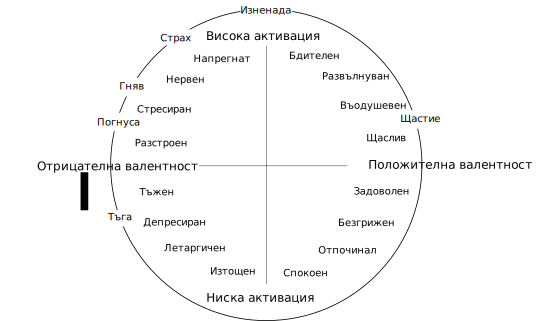
\includegraphics[width=0.8\textwidth]{valence_arousal}%
        \end{center}
        \pause
        \begin{itemize}
            \item В сигнала от реч се измерва по-лесно активацията
            \pause
            \item В сигнала от ЕЕГ се измерва по-лесно валентността
        \end{itemize}
    \end{frame}

    \begin{frame}{Нулева зона (какво е емоция)}
        \begin{columns}[T] % align columns
            \begin{column}{.38\textwidth}
                \textbf{Избрани емоции:}
                \vspace{1cm} \leavevmode \newline
                \phantom{$\bullet\ $ Гняв}
                \vspace{1cm} \leavevmode \newline
                \phantom{$\bullet\ $ Щастие}
                \vspace{1cm} \leavevmode \newline
                \phantom{$\bullet\ $ Неутрална емоция}
                \vspace{1cm} \leavevmode \newline
                \phantom{$\bullet\ $ Тъга}
            \end{column}%
            \hfill%
            \begin{column}{.60\textwidth}
                \vspace{1cm}
                \begin{center}
                    \includegraphics[width=\textwidth]{valence_arousal_empty}%
                \end{center}
            \end{column}%
        \end{columns}
    \end{frame}

    \begin{frame}{Нулева зона (какво е емоция)}
        \begin{columns}[T] % align columns
            \begin{column}{.38\textwidth}
                \textbf{Избрани емоции:}
                \vspace{1cm} \leavevmode \newline
                $\bullet\ $ Гняв
                \vspace{1cm} \leavevmode \newline
                \phantom{$\bullet\ $ Щастие}
                \vspace{1cm} \leavevmode \newline
                \phantom{$\bullet\ $ Неутрална емоция}
                \vspace{1cm} \leavevmode \newline
                \phantom{$\bullet\ $ Тъга}
            \end{column}%
            \hfill%
            \begin{column}{.60\textwidth}
                \vspace{1cm}
                \begin{center}
                    \includegraphics[width=\textwidth]{valence_arousal_a}%
                \end{center}
            \end{column}%
        \end{columns}
    \end{frame}

    \begin{frame}{Нулева зона (какво е емоция)}
        \begin{columns}[T] % align columns
            \begin{column}{.38\textwidth}
                \textbf{Избрани емоции:}
                \vspace{1cm} \leavevmode \newline
                $\bullet\ $ Гняв
                \vspace{1cm} \leavevmode \newline
                $\bullet\ $ Щастие
                \vspace{1cm} \leavevmode \newline
                \phantom{$\bullet\ $ Неутрална емоция}
                \vspace{1cm} \leavevmode \newline
                \phantom{$\bullet\ $ Тъга}
            \end{column}%
            \hfill%
            \begin{column}{.60\textwidth}
                \vspace{1cm}
                \begin{center}
                    \includegraphics[width=\textwidth]{valence_arousal_ah}%
                \end{center}
            \end{column}%
        \end{columns}
    \end{frame}

    \begin{frame}{Нулева зона (какво е емоция)}
        \begin{columns}[T] % align columns
            \begin{column}{.38\textwidth}
                \textbf{Избрани емоции:}
                \vspace{1cm} \leavevmode \newline
                $\bullet\ $ Гняв
                \vspace{1cm} \leavevmode \newline
                $\bullet\ $ Щастие
                \vspace{1cm} \leavevmode \newline
                $\bullet\ $ Неутрална емоция
                \vspace{1cm} \leavevmode \newline
                \phantom{$\bullet\ $ Тъга}
            \end{column}%
            \hfill%
            \begin{column}{.60\textwidth}
                \vspace{1cm}
                \begin{center}
                    \includegraphics[width=\textwidth]{valence_arousal_ahn}%
                \end{center}
            \end{column}%
        \end{columns}
    \end{frame}

    \begin{frame}{Нулева зона (какво е емоция)}
        \begin{columns}[T] % align columns
            \begin{column}{.38\textwidth}
                \textbf{Избрани емоции:}
                \vspace{1cm} \leavevmode \newline
                $\bullet\ $ Гняв
                \vspace{1cm} \leavevmode \newline
                $\bullet\ $ Щастие
                \vspace{1cm} \leavevmode \newline
                $\bullet\ $ Неутрална емоция
                \vspace{1cm} \leavevmode \newline
                $\bullet\ $ Тъга
            \end{column}%
            \hfill%
            \begin{column}{.60\textwidth}
                \vspace{1cm}
                \begin{center}
                    \includegraphics[width=\textwidth]{valence_arousal_ahns}%
                \end{center}
            \end{column}%
        \end{columns}
    \end{frame}

    \section{Сигнал от реч}

    \begin{frame}{Сигнал от реч - физическа обосновка}
        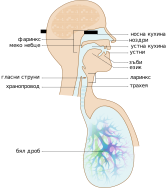
\includegraphics[width=0.48\paperwidth]{physics}%
        \hfill
        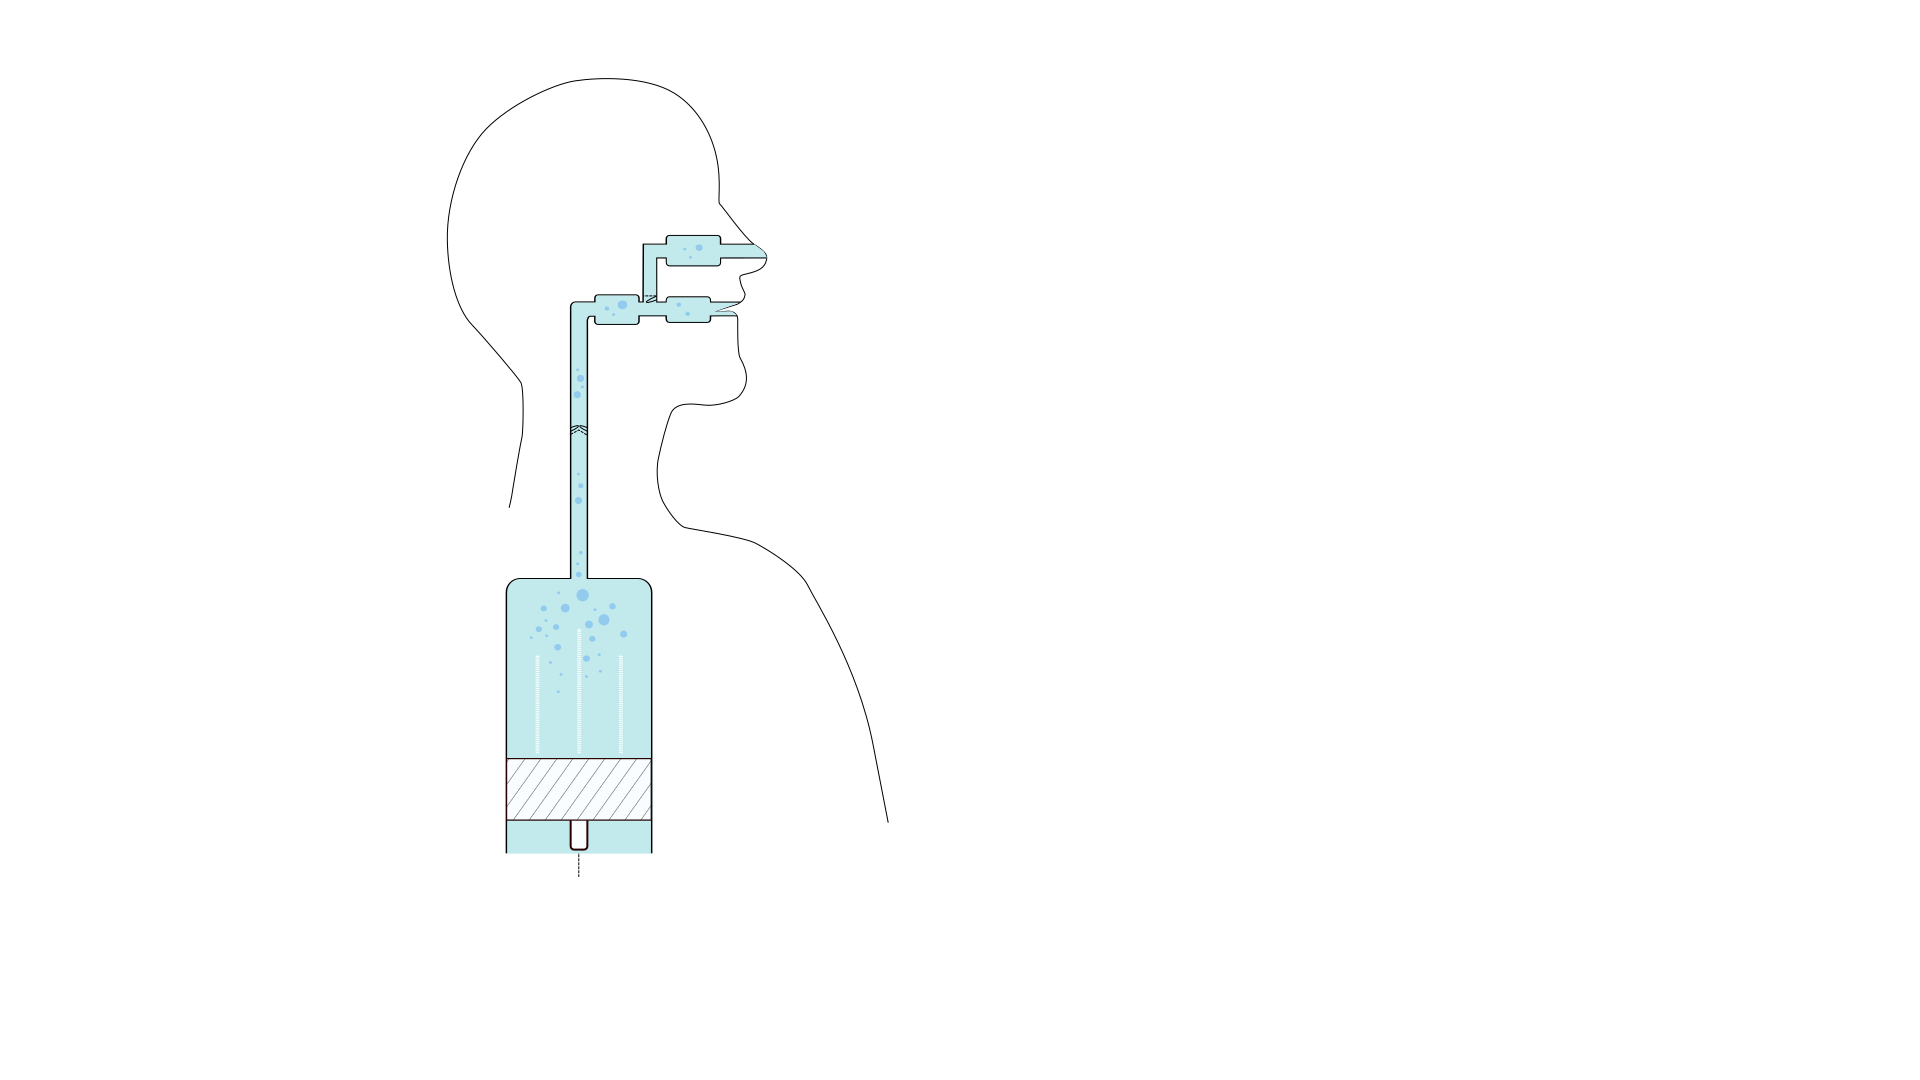
\includegraphics[width=0.28\paperwidth]{tubes}%
    \end{frame}

    \begin{frame}{Сигнал от реч - физическа обосновка}
        \centering{
            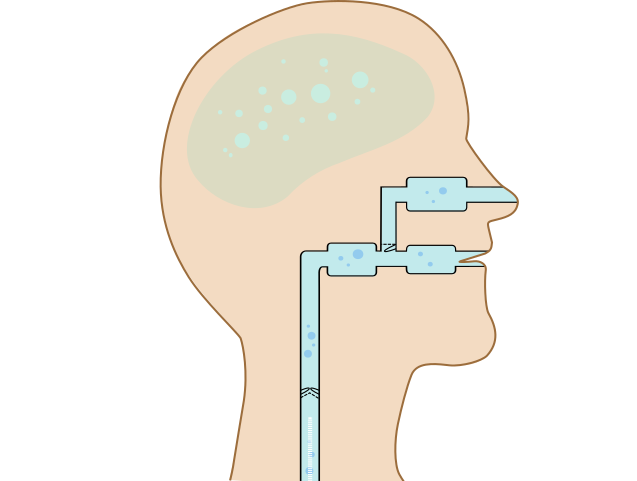
\includegraphics[height=\textheight]{glottis}%
        }
    \end{frame}

    \begin{frame}{Сигнал от реч - физическа обосновка}
    Видове звуци:
    \vspace{1cm} \leavevmode \newline
    \pause
    \begin{itemize}
        \item Озвучени - ``а''
        \pause
        \item Проходни (фрикативни) - ``с''
        \pause
        \item Преградни - ``п'' 
    \end{itemize}
    \vspace{1cm}
    \pause
    Реч \pause$\rightarrow$ думи \pause $\rightarrow$ фонеми 
    \vspace{1cm} \leavevmode \newline
    \pause
    ``Страхът стискаше гърлото, задушаваше гласа.''
    \end{frame}

    \begin{frame}{Сигнал от реч - физическа обосновка}
        \begin{itemize}
            \item Спектрални характеристики
            \pause
            \item Честотна пропускливост
        \end{itemize}
        \pause
        \centering{
            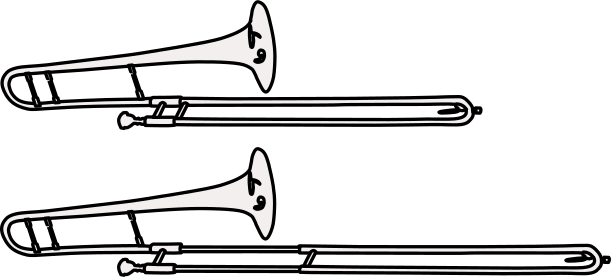
\includegraphics[width=\textwidth]{trombone}%
        }
        \pause
        \textbf{За да изследваме подлежащата емоция, трябва да изследваме спектралните свойства на статична конфигурация на вокалния тракт.}
    \end{frame}

    \begin{frame}{Сигнал от реч - модел на тръбите}
        \begin{itemize}
            \setlength\itemsep{\fill}
            \item Ще моделираме системата за производство на реч с модела на тръбите
            \pause
            \item Искаме да отделим вокалния тракт от останалите компоненти
            \pause
            \item Да разгледаме фонемата ``ъ''
            \pause
            \item Глотисът $\textbf{g}$ трепти, вокалният тракт $\textbf{v}$ филтрира сигнала, и вълната излиза и допълнително се променя от устните $\textbf{r}$ 
            \pause
            \item[$\ $] Ако  $g(t) \xleftrightarrow{\mathcal{F}\mathcal{S}} \mathcal{G}(z), v(t) \xleftrightarrow{\mathcal{F}\mathcal{S}} \mathcal{V}(z), r(t) \xleftrightarrow{\mathcal{F}\mathcal{S}} \mathcal{R}(z)$, а сигналът, който получаваме накрая, $y(t)=g(t)\ast v(t) \ast r(t), y(t) \xleftrightarrow{\mathcal{F}\mathcal{S}} \mathcal{Y}(z)$, е изпълнено, че
            \pause
            \item $\mathcal{Y}(z) = \mathcal{G}(z) \mathcal{V}(z) \mathcal{R}(z)$
        \end{itemize}
    \end{frame}

    \begin{frame}{Сигнал от реч - модел на тръбите}
    \centering{
        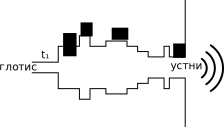
\includegraphics[width=0.7\textwidth]{vocal_tubes}%
    }
    \begin{itemize}
        \item{$c$} - скорост на звука в еластична среда
        \item{$\rho$} - плътност на въздуха в тръбите
        \item{$A$} - лицето на напречното сечение в тръба (константа)
        \item{$u = u(x, t)$} - е обемната скорост на позиция $x$ в момента $t$
        \item{$p = p(x, t)$} - е звуковото налягане
    \end{itemize}
    \end{frame}
    
    \begin{frame}[t]{Сигнал от реч - модел на тръбите}
        \begin{columns}[T]
            \begin{column}{0.48\textwidth}
                
                Уравнения на Навие-Стокс:
                \begin{flalign*}
                    -\frac{\partial\rho}{\partial x} & = \frac{\rho}{A} \frac{\partial u}{\partial t}\\
                    -\frac{\partial u}{\partial x} & = \frac{A}{\rho c^2} \frac{\partial \rho}{\partial t} 
                \end{flalign*}
            \end{column}%
            \hfill%
            \pause
            \begin{column}{0.48\textwidth}
                С решения от вида:
                \begin{flalign*}
                    & u(x, t) = \Q{u^+\B{t - \frac{x}{c}} - u^-\B{t + \frac{x}{c}}} && \\
                    & p(x, t) = \cfrac{\rho c}{A}\Q{u^+\B{t - \frac{x}{c}} + u^-\B{t + \frac{x}{c}}} &&
                \end{flalign*}
            \end{column}%
        \end{columns}
    \end{frame}

    \begin{frame}[t]{Сигнал от реч - модел на тръбите}
        \begin{columns}[T]
            \begin{column}{0.46\textwidth}
                \begin{flalign*}
                    & u(x, t) = \Q{u^+\B{t - \frac{x}{c}} - u^-\B{t + \frac{x}{c}}} && \\
                    & p(x, t) = \cfrac{\rho c}{A}\Q{u^+\B{t - \frac{x}{c}} + u^-\B{t + \frac{x}{c}}} &&
                \end{flalign*}
            \end{column}%
            \hfill%
            \pause
            \begin{column}{0.48\textwidth}
                \centering{
                    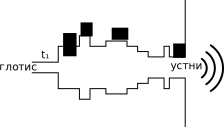
\includegraphics[width=0.7\textwidth]{vocal_tubes}%
                }
            \end{column}%
        \end{columns}
    \end{frame}

    \begin{frame}[t]{Сигнал от реч - модел на тръбите}
        \begin{columns}[T]
            \begin{column}{0.48\textwidth}
                \begin{flalign*}
                    & u_k(x, t) = \Q{u_k^+\B{t - \frac{x}{c}} - u_k^-\B{t + \frac{x}{c}}} && \\
                    & p_k(x, t) = \cfrac{\rho c}{A_k}\Q{u_k^+\B{t - \frac{x}{c}} + u_k^-\B{t + \frac{x}{c}}} &&
                \end{flalign*}
            \end{column}%
            \hfill%
            \begin{column}{0.48\textwidth}
                \centering{
                    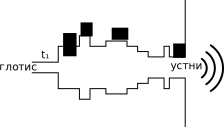
\includegraphics[width=0.7\textwidth]{vocal_tubes}%
                }
            \end{column}%
        \end{columns}
    \end{frame}

    \begin{frame}[t]{Сигнал от реч - модел на тръбите}
        \begin{columns}[T]
            \begin{column}{0.48\textwidth}
                \begin{flalign*}
                    & u_k(x, t) = \Q{u_k^+\B{t - \frac{x}{c}} - u_k^-\B{t + \frac{x}{c}}} && \\
                    & p_k(x, t) = \cfrac{\rho c}{A_k}\Q{u_k^+\B{t - \frac{x}{c}} + u_k^-\B{t + \frac{x}{c}}} &&
                \end{flalign*}
            \end{column}%
            \hfill%
            \begin{column}{0.26\textwidth}
                \begin{flalign*}
                    & u_k(l_k, t)= u_{k+1}(0, t) && \\
                    & p_k(l_k, t)= p_{k+1}(0, t) &&
                \end{flalign*}
            \end{column}%
            \hfill
            \begin{column}{0.22\textwidth}
            \end{column}%
        \end{columns}
        \pause
        \begin{flalign*}
            & u_k^+\B{t - \cfrac{l_k}{c}} - u_k^{-}\B{t + \cfrac{l_k}{c}} = u_{k+1}^{+}(t) - u_{k+1}^{-}(t) &&\\
            & \cfrac{A_{k+1}}{A_{k}}\Q{u_{k}^{+}\B{t - \cfrac{l_k}{c}} + u_{k}^{-}\B{t + \cfrac{l_k}{c}}} = u_{k+1}^{+}(t) + u_{k+1}^{-}(t) &&
        \end{flalign*}  
    \end{frame}

    \begin{frame}[t]{Сигнал от реч - модел на тръбите}
        \begin{columns}[T]
            \begin{column}{0.48\textwidth}
                \begin{flalign*}
                    & u_k(x, t) = \Q{u_k^+\B{t - \frac{x}{c}} - u_k^-\B{t + \frac{x}{c}}} && \\
                    & p_k(x, t) = \cfrac{\rho c}{A_k}\Q{u_k^+\B{t - \frac{x}{c}} + u_k^-\B{t + \frac{x}{c}}} &&
                \end{flalign*}
            \end{column}%
            \hfill%
            \begin{column}{0.26\textwidth}
                \begin{flalign*}
                    & u_k(l_k, t)= u_{k+1}(0, t) && \\
                    & p_k(l_k, t)= p_{k+1}(0, t) &&
                \end{flalign*}
            \end{column}%
            \hfill
            \begin{column}{0.22\textwidth}
            \end{column}%
        \end{columns}
        \begin{flalign*}
            & u_k^+\B{t - \cfrac{l_k}{c}} - u_k^{-}\B{t + \cfrac{l_k}{c}} = u_{k+1}^{+}(t) - u_{k+1}^{-}(t) &&\\
            & \cfrac{A_{k+1}}{A_{k}}\Q{u_{k}^{+}\B{t - \cfrac{l_k}{c}} + u_{k}^{-}\B{t + \cfrac{l_k}{c}}} = u_{k+1}^{+}(t) + u_{k+1}^{-}(t) \qquad \tau_k = \cfrac{l_k}{c} &&
        \end{flalign*}  
    \end{frame}

    \begin{frame}[t]{Сигнал от реч - модел на тръбите}
        \begin{columns}[T]
            \begin{column}{0.48\textwidth}
                \begin{flalign*}
                    & u_k(x, t) = \Q{u_k^+\B{t - \frac{x}{c}} - u_k^-\B{t + \frac{x}{c}}} && \\
                    & p_k(x, t) = \cfrac{\rho c}{A_k}\Q{u_k^+\B{t - \frac{x}{c}} + u_k^-\B{t + \frac{x}{c}}} &&
                \end{flalign*}
            \end{column}%
            \hfill%
            \begin{column}{0.26\textwidth}
                \begin{flalign*}
                    & u_k(l_k, t) = u_{k+1}(0, t) && \\
                    & p_k(l_k, t) = p_{k+1}(0, t) &&
                \end{flalign*}
            \end{column}%
            \hfill
            \begin{column}{0.22\textwidth}
            \end{column}%
        \end{columns}
        \begin{flalign*}
            & u_k^+\B{t - \tau_k} - u_k^{-}\B{t + \tau_k} = u_{k+1}^{+}(t) - u_{k+1}^{-}(t) &&\\
            & \cfrac{A_{k+1}}{A_{k}}\Q{u_{k}^{+}\B{t - \tau_k} + u_{k}^{-}\B{t + \tau_k}} = u_{k+1}^{+}(t) + u_{k+1}^{-}(t) &&
        \end{flalign*}
    \end{frame}

    \begin{frame}[t]{Сигнал от реч - модел на тръбите}
        \begin{columns}[T]
            \begin{column}{0.48\textwidth}
                \begin{flalign*}
                    & u_k(x, t) = \Q{u_k^+\B{t - \frac{x}{c}} - u_k^-\B{t + \frac{x}{c}}} && \\
                    & p_k(x, t) = \cfrac{\rho c}{A_k}\Q{u_k^+\B{t - \frac{x}{c}} + u_k^-\B{t + \frac{x}{c}}} &&
                \end{flalign*}
            \end{column}%
            \hfill%
            \begin{column}{0.26\textwidth}
                \begin{flalign*}
                    & u_k(l_k, t) = u_{k+1}(0, t) && \\
                    & p_k(l_k, t) = p_{k+1}(0, t) &&
                \end{flalign*}
            \end{column}%
            \hfill
            \begin{column}{0.22\textwidth}
            \end{column}%
        \end{columns}
        \begin{flalign*}
            & {\color{mypink}u_k^+\B{t - \tau_k} - \boldsymbol{u_k^{-}\B{t + \tau_k}} = u_{k+1}^{+}(t) - u_{k+1}^{-}(t)} &&\\
            & \cfrac{A_{k+1}}{A_{k}}\Q{u_{k}^{+}\B{t - \tau_k} + u_{k}^{-}\B{t + \tau_k}} = u_{k+1}^{+}(t) + u_{k+1}^{-}(t) &&
        \end{flalign*}
        \pause
        \begin{flalign*}
            & u_k^{-}\B{t + \tau_k} = u_k^+\B{t - \tau_k} - u_{k+1}^{+}(t) + u_{k+1}^{-}(t) &&
        \end{flalign*}
        \vspace{1.7cm}
    \end{frame}

    \begin{frame}[t]{Сигнал от реч - модел на тръбите}
        \begin{columns}[T]
            \begin{column}{0.48\textwidth}
                \begin{flalign*}
                    & u_k(x, t) = \Q{u_k^+\B{t - \frac{x}{c}} - u_k^-\B{t + \frac{x}{c}}} && \\
                    & p_k(x, t) = \cfrac{\rho c}{A_k}\Q{u_k^+\B{t - \frac{x}{c}} + u_k^-\B{t + \frac{x}{c}}} &&
                \end{flalign*}
            \end{column}%
            \hfill%
            \begin{column}{0.26\textwidth}
                \begin{flalign*}
                    & u_k(l_k, t) = u_{k+1}(0, t) && \\
                    & p_k(l_k, t) = p_{k+1}(0, t) &&
                \end{flalign*}
            \end{column}%
            \hfill
            \begin{column}{0.22\textwidth}
            \end{column}%
        \end{columns}
        \begin{flalign*}
            & u_k^+\B{t - \tau_k} - u_k^{-}\B{t + \tau_k} = u_{k+1}^{+}(t) - u_{k+1}^{-}(t) &&\\
            & {\color{mypink}\cfrac{A_{k+1}}{A_{k}}\Q{u_{k}^{+}\B{t - \tau_k} + \boldsymbol{u_{k}^{-}\B{t + \tau_k}}} = u_{k+1}^{+}(t) + u_{k+1}^{-}(t)} &&
        \end{flalign*}
        \begin{flalign*}
            & {\color{mypink} \boldsymbol{u_k^{-}\B{t + \tau_k}}} = u_k^+\B{t - \tau_k} - u_{k+1}^{+}(t) + u_{k+1}^{-}(t) &&
        \end{flalign*}
        и изразяваме $u_{k+1}^{+}$
    \end{frame}
    
    \begin{frame}[t]{Сигнал от реч - модел на тръбите}
        \begin{columns}[T]
            \begin{column}{0.48\textwidth}
                \begin{flalign*}
                    & u_k(x, t) = \Q{u_k^+\B{t - \frac{x}{c}} - u_k^-\B{t + \frac{x}{c}}} && \\
                    & p_k(x, t) = \cfrac{\rho c}{A_k}\Q{u_k^+\B{t - \frac{x}{c}} + u_k^-\B{t + \frac{x}{c}}} &&
                \end{flalign*}
            \end{column}%
            \hfill%
            \begin{column}{0.26\textwidth}
                \begin{flalign*}
                    & u_k(l_k, t) = u_{k+1}(0, t) && \\
                    & p_k(l_k, t) = p_{k+1}(0, t) &&
                \end{flalign*}
            \end{column}%
            \hfill
            \begin{column}{0.22\textwidth}
            \end{column}%
        \end{columns}
        \begin{flalign*}
            & u_k^+\B{t - \tau_k} - u_k^{-}\B{t + \tau_k} = u_{k+1}^{+}(t) - u_{k+1}^{-}(t) &&\\
            & \cfrac{A_{k+1}}{A_{k}}\Q{u_{k}^{+}\B{t - \tau_k} + u_{k}^{-}\B{t + \tau_k} = u_{k+1}^{+}(t) + u_{k+1}^{-}(t)} &&
        \end{flalign*}
        \begin{flalign*}
            & u_k^{-}\B{t + \tau_k} = u_k^+\B{t - \tau_k} - u_{k+1}^{+}(t) + u_{k+1}^{-}(t) &&\\
            & u_{k+1}^{+}(t) = u_{k}^{+}(t - \tau_k)\Q{\frac{2A_{k+1}}{A_k + A_{k+1}}} + u_{k+1}^{-}(t)\Q{\frac{A_{k+1} - A_k}{A_k + A_{k+1}}} &&
        \end{flalign*}
        \pause
        \begin{columns}[T]
            \begin{column}{0.48\textwidth}
                $t_k = \cfrac{2A_{k+1}}{A_k + A_{k+1}}$
            \end{column}%
            \hfill%
            \pause
            \begin{column}{0.48\textwidth}
                $r_k = \cfrac{A_{k+1} - A_k}{A_k + A_{k+1}}$
            \end{column}%
        \end{columns}
    \end{frame}

    \begin{frame}[t]{Сигнал от реч - модел на тръбите}
        \begin{columns}[T]
            \begin{column}{0.48\textwidth}
                \begin{flalign*}
                    & u_k(x, t) = \Q{u_k^+\B{t - \frac{x}{c}} - u_k^-\B{t + \frac{x}{c}}} && \\
                    & p_k(x, t) = \cfrac{\rho c}{A_k}\Q{u_k^+\B{t - \frac{x}{c}} + u_k^-\B{t + \frac{x}{c}}} &&
                \end{flalign*}
            \end{column}%
            \hfill%
            \begin{column}{0.26\textwidth}
                \begin{flalign*}
                    & u_k(l_k, t) = u_{k+1}(0, t) && \\
                    & p_k(l_k, t) = p_{k+1}(0, t) &&
                \end{flalign*}
            \end{column}%
            \hfill
            \begin{column}{0.22\textwidth}
                \begin{flalign*}
                    & r_k = \cfrac{A_{k+1} - A_k}{A_k + A_{k+1}} &&
                \end{flalign*}
            \end{column}%
        \end{columns}
        \begin{flalign*}
            & u_k^+\B{t - \tau_k} - u_k^{-}\B{t + \tau_k} = u_{k+1}^{+}(t) - u_{k+1}^{-}(t) &&\\
            & \cfrac{A_{k+1}}{A_{k}}\Q{u_{k}^{+}\B{t - \tau_k} + u_{k}^{-}\B{t + \tau_k} = u_{k+1}^{+}(t) + u_{k+1}^{-}(t)} &&
        \end{flalign*}
        \begin{flalign*}
            & u_k^{-}\B{t + \tau_k} = u_k^+\B{t - \tau_k} - u_{k+1}^{+}(t) + u_{k+1}^{-}(t) &&\\
            & u_{k+1}^{+}(t) = u_{k}^{+}(t - \tau_k)\Q{\frac{2A_{k+1}}{A_k + A_{k+1}}} + u_{k+1}^{-}(t)\Q{\frac{A_{k+1} - A_k}{A_k + A_{k+1}}} &&
        \end{flalign*}
        \begin{columns}[T]
            \begin{column}{0.48\textwidth}
                $t_k = \cfrac{2A_{k+1}}{A_k + A_{k+1}}$
            \end{column}%
            \hfill%
            \begin{column}{0.48\textwidth}
                $r_k = \cfrac{A_{k+1} - A_k}{A_k + A_{k+1}}$
            \end{column}%
        \end{columns}
    \end{frame}
      
    \begin{frame}[t]{Сигнал от реч - модел на тръбите}
        \begin{columns}[T]
            \begin{column}{0.48\textwidth}
                \begin{flalign*}
                    & u_k(x, t) = \Q{u_k^+\B{t - \frac{x}{c}} - u_k^-\B{t + \frac{x}{c}}} && \\
                    & p_k(x, t) = \cfrac{\rho c}{A_k}\Q{u_k^+\B{t - \frac{x}{c}} + u_k^-\B{t + \frac{x}{c}}} &&
                \end{flalign*}
            \end{column}%
            \hfill%
            \begin{column}{0.26\textwidth}
                \begin{flalign*}
                    & u_k(l_k, t) = u_{k+1}(0, t) && \\
                    & p_k(l_k, t) = p_{k+1}(0, t) &&
                \end{flalign*}
            \end{column}%
            \hfill
            \begin{column}{0.22\textwidth}
                \begin{flalign*}
                    & r_k = \cfrac{A_{k+1} - A_k}{A_k + A_{k+1}} &&
                \end{flalign*}
            \end{column}%
        \end{columns}
        \begin{flalign*}
            & u_k^+\B{t - \tau_k} - u_k^{-}\B{t + \tau_k} = u_{k+1}^{+}(t) - u_{k+1}^{-}(t) &&\\
            & \cfrac{A_{k+1}}{A_{k}}\Q{u_{k}^{+}\B{t - \tau_k} + u_{k}^{-}\B{t + \tau_k} = u_{k+1}^{+}(t) + u_{k+1}^{-}(t)} &&
        \end{flalign*}
        \begin{flalign*}
            & u_k^{-}\B{t + \tau_k} = u_k^+\B{t - \tau_k} - u_{k+1}^{+}(t) + u_{k+1}^{-}(t) &&\\
            & {\color{mypink}u_{k+1}^{+}(t) = u_{k}^{+}(t - \tau_k)\Q{\frac{2A_{k+1}}{A_k + A_{k+1}}} + u_{k+1}^{-}(t)\Q{\frac{A_{k+1} - A_k}{A_k + A_{k+1}}}} &&
        \end{flalign*}
    \end{frame}
            
    \begin{frame}[t]{Сигнал от реч - модел на тръбите}
        \begin{columns}[T]
            \begin{column}{0.48\textwidth}
                \begin{flalign*}
                    & u_k(x, t) = \Q{u_k^+\B{t - \frac{x}{c}} - u_k^-\B{t + \frac{x}{c}}} && \\
                    & p_k(x, t) = \cfrac{\rho c}{A_k}\Q{u_k^+\B{t - \frac{x}{c}} + u_k^-\B{t + \frac{x}{c}}} &&
                \end{flalign*}
            \end{column}%
            \hfill%
            \begin{column}{0.26\textwidth}
                \begin{flalign*}
                    & u_k(l_k, t) = u_{k+1}(0, t) && \\
                    & p_k(l_k, t) = p_{k+1}(0, t) &&
                \end{flalign*}
            \end{column}%
            \hfill
            \begin{column}{0.22\textwidth}
                \begin{flalign*}
                    & r_k = \cfrac{A_{k+1} - A_k}{A_k + A_{k+1}} &&
                \end{flalign*}
            \end{column}%
        \end{columns}
        \begin{flalign*}
            & u_k^+\B{t - \tau_k} - u_k^{-}\B{t + \tau_k} = u_{k+1}^{+}(t) - u_{k+1}^{-}(t) &&\\
            & \cfrac{A_{k+1}}{A_{k}}\Q{u_{k}^{+}\B{t - \tau_k} + u_{k}^{-}\B{t + \tau_k} = u_{k+1}^{+}(t) + u_{k+1}^{-}(t)} &&
        \end{flalign*}
        \begin{flalign*}
            & {\color{mypink}u_{k+1}^{+}(t) = \boldsymbol{u_{k}^{+}(t - \tau_k)}\Q{\frac{2A_{k+1}}{A_k + A_{k+1}}} + u_{k+1}^{-}(t)\Q{\frac{A_{k+1} - A_k}{A_k + A_{k+1}}}} &&
        \end{flalign*}
    \end{frame}
    
    \begin{frame}[t]{Сигнал от реч - модел на тръбите}
        \begin{columns}[T]
            \begin{column}{0.48\textwidth}
                \begin{flalign*}
                    & u_k(x, t) = \Q{u_k^+\B{t - \frac{x}{c}} - u_k^-\B{t + \frac{x}{c}}} && \\
                    & p_k(x, t) = \cfrac{\rho c}{A_k}\Q{u_k^+\B{t - \frac{x}{c}} + u_k^-\B{t + \frac{x}{c}}} &&
                \end{flalign*}
            \end{column}%
            \hfill%
            \begin{column}{0.26\textwidth}
                \begin{flalign*}
                    & u_k(l_k, t) = u_{k+1}(0, t) && \\
                    & p_k(l_k, t) = p_{k+1}(0, t) &&
                \end{flalign*}
            \end{column}%
            \hfill
            \begin{column}{0.22\textwidth}
                \begin{flalign*}
                    & r_k = \cfrac{A_{k+1} - A_k}{A_k + A_{k+1}} &&
                \end{flalign*}
            \end{column}%
        \end{columns}
        \begin{flalign*}
            & u_k^+\B{t - \tau_k} - u_k^{-}\B{t + \tau_k} = u_{k+1}^{+}(t) - u_{k+1}^{-}(t) &&\\
            & \cfrac{A_{k+1}}{A_{k}}\Q{u_{k}^{+}\B{t - \tau_k} + u_{k}^{-}\B{t + \tau_k} = u_{k+1}^{+}(t) + u_{k+1}^{-}(t)} &&
        \end{flalign*}
        \begin{flalign*}
            & {\color{mypink}u_{k+1}^{+}(t) = \boldsymbol{u_{k}^{+}(t - \tau_k)}\Q{\frac{2A_{k+1}}{A_k + A_{k+1}}} + u_{k+1}^{-}(t)\Q{\frac{A_{k+1} - A_k}{A_k + A_{k+1}}}} && \\
            & u_k^{+}(t - \tau_k) = u_{k+1}^{+}(t)\Q{\frac{A_k + A_{k+1}}{2A_{k+1}}} + u_{k+1}^{-}(t)\Q{\frac{A_k - A_{k+1}}{2A_{k+1}}} &&
        \end{flalign*}
    \end{frame}

    \begin{frame}[t]{Сигнал от реч - модел на тръбите}
    \begin{columns}[T]
        \begin{column}{0.48\textwidth}
            \begin{flalign*}
                & u_k(x, t) = \Q{u_k^+\B{t - \frac{x}{c}} - u_k^-\B{t + \frac{x}{c}}} && \\
                & p_k(x, t) = \cfrac{\rho c}{A_k}\Q{u_k^+\B{t - \frac{x}{c}} + u_k^-\B{t + \frac{x}{c}}} &&
            \end{flalign*}
        \end{column}%
        \hfill%
        \begin{column}{0.26\textwidth}
            \begin{flalign*}
                & u_k(l_k, t) = u_{k+1}(0, t) && \\
                & p_k(l_k, t) = p_{k+1}(0, t) &&
            \end{flalign*}
        \end{column}%
        \hfill
        \begin{column}{0.22\textwidth}
            \begin{flalign*}
                & r_k = \cfrac{A_{k+1} - A_k}{A_k + A_{k+1}} &&
            \end{flalign*}
        \end{column}%
    \end{columns}
    \begin{flalign*}
        & u_k^+\B{t - \tau_k} - u_k^{-}\B{t + \tau_k} = u_{k+1}^{+}(t) - u_{k+1}^{-}(t) &&\\
        & \cfrac{A_{k+1}}{A_{k}}\Q{u_{k}^{+}\B{t - \tau_k} + u_{k}^{-}\B{t + \tau_k} = u_{k+1}^{+}(t) + u_{k+1}^{-}(t)} &&
    \end{flalign*}
    \begin{flalign*}
        & u_{k+1}^{+}(t) = u_{k}^{+}(t - \tau_k)\Q{\frac{2A_{k+1}}{A_k + A_{k+1}}} + u_{k+1}^{-}(t)\Q{\frac{A_{k+1} - A_k}{A_k + A_{k+1}}} && \\
        & u_k^{+}(t - \tau_k) = u_{k+1}^{+}(t)\Q{\frac{A_k + A_{k+1}}{2A_{k+1}}} + u_{k+1}^{-}(t)\Q{\frac{A_k - A_{k+1}}{2A_{k+1}}} &&
    \end{flalign*}
    \end{frame}

    \begin{frame}[t]{Сигнал от реч - модел на тръбите}
    \begin{columns}[T]
        \begin{column}{0.48\textwidth}
            \begin{flalign*}
                & u_k(x, t) = \Q{u_k^+\B{t - \frac{x}{c}} - u_k^-\B{t + \frac{x}{c}}} && \\
                & p_k(x, t) = \cfrac{\rho c}{A_k}\Q{u_k^+\B{t - \frac{x}{c}} + u_k^-\B{t + \frac{x}{c}}} &&
            \end{flalign*}
        \end{column}%
        \hfill%
        \begin{column}{0.26\textwidth}
            \begin{flalign*}
                & u_k(l_k, t) = u_{k+1}(0, t) && \\
                & p_k(l_k, t) = p_{k+1}(0, t) &&
            \end{flalign*}
        \end{column}%
        \hfill
        \begin{column}{0.22\textwidth}
            \begin{flalign*}
                & r_k = \cfrac{A_{k+1} - A_k}{A_k + A_{k+1}} &&
            \end{flalign*}
        \end{column}%
    \end{columns}
    \begin{flalign*}
        & {\color{mypink} u_k^+\B{t - \tau_k} - \boldsymbol{u_k^{-}\B{t + \tau_k}} = u_{k+1}^{+}(t) - u_{k+1}^{-}(t)} &&\\
        & \cfrac{A_{k+1}}{A_{k}}\Q{u_{k}^{+}\B{t - \tau_k} + u_{k}^{-}\B{t + \tau_k} = u_{k+1}^{+}(t) + u_{k+1}^{-}(t)} &&
    \end{flalign*}
    \begin{flalign*}
        & u_{k+1}^{+}(t) = u_{k}^{+}(t - \tau_k)\Q{\frac{2A_{k+1}}{A_k + A_{k+1}}} + u_{k+1}^{-}(t)\Q{\frac{A_{k+1} - A_k}{A_k + A_{k+1}}} && \\
        & {\color{mypink} u_k^{+}(t - \tau_k)} = u_{k+1}^{+}(t)\Q{\frac{A_k + A_{k+1}}{2A_{k+1}}} + u_{k+1}^{-}(t)\Q{\frac{A_k - A_{k+1}}{2A_{k+1}}} &&
    \end{flalign*}
    \end{frame}

    \begin{frame}[t]{Сигнал от реч - модел на тръбите}
    \begin{columns}[T]
        \begin{column}{0.48\textwidth}
            \begin{flalign*}
                & u_k(x, t) = \Q{u_k^+\B{t - \frac{x}{c}} - u_k^-\B{t + \frac{x}{c}}} && \\
                & p_k(x, t) = \cfrac{\rho c}{A_k}\Q{u_k^+\B{t - \frac{x}{c}} + u_k^-\B{t + \frac{x}{c}}} &&
            \end{flalign*}
        \end{column}%
        \hfill%
        \begin{column}{0.26\textwidth}
            \begin{flalign*}
                & u_k(l_k, t) = u_{k+1}(0, t) && \\
                & p_k(l_k, t) = p_{k+1}(0, t) &&
            \end{flalign*}
        \end{column}%
        \hfill
        \begin{column}{0.22\textwidth}
            \begin{flalign*}
                & r_k = \cfrac{A_{k+1} - A_k}{A_k + A_{k+1}} &&
            \end{flalign*}
        \end{column}%
    \end{columns}
    \begin{flalign*}
        & {\color{mypink} u_k^+\B{t - \tau_k} - \boldsymbol{u_k^{-}\B{t + \tau_k}} = u_{k+1}^{+}(t) - u_{k+1}^{-}(t)} &&\\
        & \cfrac{A_{k+1}}{A_{k}}\Q{u_{k}^{+}\B{t - \tau_k} + u_{k}^{-}\B{t + \tau_k} = u_{k+1}^{+}(t) + u_{k+1}^{-}(t)} &&
    \end{flalign*}
    \begin{flalign*}
        & u_{k+1}^{+}(t) = u_{k}^{+}(t - \tau_k)\Q{\frac{2A_{k+1}}{A_k + A_{k+1}}} + u_{k+1}^{-}(t)\Q{\frac{A_{k+1} - A_k}{A_k + A_{k+1}}} && \\
        & u_k^{+}(t - \tau_k) = u_{k+1}^{+}(t)\Q{\frac{A_k + A_{k+1}}{2A_{k+1}}} + u_{k+1}^{-}(t)\Q{\frac{A_k - A_{k+1}}{2A_{k+1}}} &&\\
        & u_k^{-}(t + \tau_k) = u_{k+1}^{+}(t)\Q{\frac{A_k - A_{k+1}}{2A_{k+1}}} + u_{k+1}^{-}(t)\Q{\frac{A_k + A_{k+1}}{2A_{k+1}}} &&
    \end{flalign*}
    \end{frame}

    \begin{frame}[t]{Сигнал от реч - модел на тръбите}
    \begin{columns}[T]
        \begin{column}{0.48\textwidth}
            \begin{flalign*}
                & u_k(x, t) = \Q{u_k^+\B{t - \frac{x}{c}} - u_k^-\B{t + \frac{x}{c}}} && \\
                & p_k(x, t) = \cfrac{\rho c}{A_k}\Q{u_k^+\B{t - \frac{x}{c}} + u_k^-\B{t + \frac{x}{c}}} &&
            \end{flalign*}
        \end{column}%
        \hfill%
        \begin{column}{0.26\textwidth}
            \begin{flalign*}
                & u_k(l_k, t) = u_{k+1}(0, t) && \\
                & p_k(l_k, t) = p_{k+1}(0, t) &&
            \end{flalign*}
        \end{column}%
        \hfill
        \begin{column}{0.22\textwidth}
            \begin{flalign*}
                & r_k = \cfrac{A_{k+1} - A_k}{A_k + A_{k+1}} &&
            \end{flalign*}
        \end{column}%
    \end{columns}
    \begin{flalign*}
        & u_k^+\B{t - \tau_k} - u_k^{-}\B{t + \tau_k} = u_{k+1}^{+}(t) - u_{k+1}^{-}(t) &&\\
        & \cfrac{A_{k+1}}{A_{k}}\Q{u_{k}^{+}\B{t - \tau_k} + u_{k}^{-}\B{t + \tau_k} = u_{k+1}^{+}(t) + u_{k+1}^{-}(t)} &&
    \end{flalign*}
    \begin{flalign*}
        & u_{k+1}^{+}(t) = u_{k}^{+}(t - \tau_k)\Q{\frac{2A_{k+1}}{A_k + A_{k+1}}} + u_{k+1}^{-}(t)\Q{\frac{A_{k+1} - A_k}{A_k + A_{k+1}}} && \\
        & u_k^{+}(t - \tau_k) = u_{k+1}^{+}(t)\Q{\frac{A_k + A_{k+1}}{2A_{k+1}}} + u_{k+1}^{-}(t)\Q{\frac{A_k - A_{k+1}}{2A_{k+1}}} &&\\
        & u_k^{-}(t + \tau_k) = u_{k+1}^{+}(t)\Q{\frac{A_k - A_{k+1}}{2A_{k+1}}} + u_{k+1}^{-}(t)\Q{\frac{A_k + A_{k+1}}{2A_{k+1}}} &&
    \end{flalign*}
    \end{frame}

    \begin{frame}[t]{Сигнал от реч - модел на тръбите}
    \begin{columns}[T]
        \begin{column}{0.48\textwidth}
            \begin{flalign*}
                & u_k(x, t) = \Q{u_k^+\B{t - \frac{x}{c}} - u_k^-\B{t + \frac{x}{c}}} && \\
                & p_k(x, t) = \cfrac{\rho c}{A_k}\Q{u_k^+\B{t - \frac{x}{c}} + u_k^-\B{t + \frac{x}{c}}} &&
            \end{flalign*}
        \end{column}%
        \hfill%
        \begin{column}{0.26\textwidth}
            \begin{flalign*}
                & u_k(l_k, t) = u_{k+1}(0, t) && \\
                & p_k(l_k, t) = p_{k+1}(0, t) &&
            \end{flalign*}
        \end{column}%
        \hfill
        \begin{column}{0.22\textwidth}
            \begin{flalign*}
                & r_k = \cfrac{A_{k+1} - A_k}{A_k + A_{k+1}} &&
            \end{flalign*}
        \end{column}%
    \end{columns}
    \begin{flalign*}
        & u_k^+\B{t - \tau_k} - u_k^{-}\B{t + \tau_k} = u_{k+1}^{+}(t) - u_{k+1}^{-}(t) &&\\
        & \cfrac{A_{k+1}}{A_{k}}\Q{u_{k}^{+}\B{t - \tau_k} + u_{k}^{-}\B{t + \tau_k} = u_{k+1}^{+}(t) + u_{k+1}^{-}(t)} &&
    \end{flalign*}
    \begin{flalign*}
        & u_{k+1}^{+}(t) = u_{k}^{+}(t - \tau_k)\Q{\frac{2A_{k+1}}{A_k + A_{k+1}}} + u_{k+1}^{-}(t)\Q{\frac{A_{k+1} - A_k}{A_k + A_{k+1}}} && \\
        & {\color{mypink} u_k^{+}(t - \tau_k) = u_{k+1}^{+}(t)\Q{\frac{A_k + A_{k+1}}{2A_{k+1}}} + u_{k+1}^{-}(t)\Q{\frac{A_k - A_{k+1}}{2A_{k+1}}}} &&\\
        & {\color{mypink} u_k^{-}(t + \tau_k) = u_{k+1}^{+}(t)\Q{\frac{A_k - A_{k+1}}{2A_{k+1}}} + u_{k+1}^{-}(t)\Q{\frac{A_k + A_{k+1}}{2A_{k+1}}}} &&
    \end{flalign*}
    \end{frame}

    \begin{frame}[t]{Сигнал от реч - модел на тръбите}
    \begin{columns}[T]
        \begin{column}{0.48\textwidth}
            \begin{flalign*}
                & u_k(x, t) = \Q{u_k^+\B{t - \frac{x}{c}} - u_k^-\B{t + \frac{x}{c}}} && \\
                & p_k(x, t) = \cfrac{\rho c}{A_k}\Q{u_k^+\B{t - \frac{x}{c}} + u_k^-\B{t + \frac{x}{c}}} &&
            \end{flalign*}
        \end{column}%
        \hfill%
        \begin{column}{0.26\textwidth}
            \begin{flalign*}
                & u_k(l_k, t) = u_{k+1}(0, t) && \\
                & p_k(l_k, t) = p_{k+1}(0, t) &&
            \end{flalign*}
        \end{column}%
        \hfill
        \begin{column}{0.22\textwidth}
            \begin{flalign*}
                & r_k = \cfrac{A_{k+1} - A_k}{A_k + A_{k+1}} &&
            \end{flalign*}
        \end{column}%
    \end{columns}
    \begin{flalign*}
        & u_k^{+}(t - \tau_k) = u_{k+1}^{+}(t)\Q{\frac{A_k + A_{k+1}}{2A_{k+1}}} + u_{k+1}^{-}(t)\Q{\frac{A_k - A_{k+1}}{2A_{k+1}}} &&\\
        & u_k^{-}(t + \tau_k) = u_{k+1}^{+}(t)\Q{\frac{A_k - A_{k+1}}{2A_{k+1}}} + u_{k+1}^{-}(t)\Q{\frac{A_k + A_{k+1}}{2A_{k+1}}} &&
    \end{flalign*}
    \end{frame}

    \begin{frame}[t]{Сигнал от реч - модел на тръбите}
    \begin{columns}[T]
        \begin{column}{0.48\textwidth}
            \begin{flalign*}
                & u_k(x, t) = \Q{u_k^+\B{t - \frac{x}{c}} - u_k^-\B{t + \frac{x}{c}}} && \\
                & p_k(x, t) = \cfrac{\rho c}{A_k}\Q{u_k^+\B{t - \frac{x}{c}} + u_k^-\B{t + \frac{x}{c}}} &&
            \end{flalign*}
        \end{column}%
        \hfill%
        \begin{column}{0.26\textwidth}
            \begin{flalign*}
                & u_k(l_k, t) = u_{k+1}(0, t) && \\
                & p_k(l_k, t) = p_{k+1}(0, t) &&
            \end{flalign*}
        \end{column}%
        \hfill
        \begin{column}{0.22\textwidth}
            \begin{flalign*}
                & {\color{mypink}r_k = \cfrac{A_{k+1} - A_k}{A_k + A_{k+1}}} &&
            \end{flalign*}
        \end{column}%
    \end{columns}
    \begin{flalign*}
        & u_k^{+}(t - \tau_k) = u_{k+1}^{+}(t)\Q{\frac{A_k + A_{k+1}}{2A_{k+1}}} + u_{k+1}^{-}(t)\Q{\frac{A_k - A_{k+1}}{2A_{k+1}}} &&\\
        & u_k^{-}(t + \tau_k) = u_{k+1}^{+}(t)\Q{\frac{A_k - A_{k+1}}{2A_{k+1}}} + u_{k+1}^{-}(t)\Q{\frac{A_k + A_{k+1}}{2A_{k+1}}} &&
    \end{flalign*}
    \end{frame}

    \begin{frame}[t]{Сигнал от реч - модел на тръбите}
    \begin{columns}[T]
        \begin{column}{0.48\textwidth}
            \begin{flalign*}
                & u_k(x, t) = \Q{u_k^+\B{t - \frac{x}{c}} - u_k^-\B{t + \frac{x}{c}}} && \\
                & p_k(x, t) = \cfrac{\rho c}{A_k}\Q{u_k^+\B{t - \frac{x}{c}} + u_k^-\B{t + \frac{x}{c}}} &&
            \end{flalign*}
        \end{column}%
        \hfill%
        \begin{column}{0.26\textwidth}
            \begin{flalign*}
                & u_k(l_k, t) = u_{k+1}(0, t) && \\
                & p_k(l_k, t) = p_{k+1}(0, t) &&
            \end{flalign*}
        \end{column}%
        \hfill
        \begin{column}{0.22\textwidth}
            \begin{flalign*}
                & {\color{mypink}r_k = \cfrac{A_{k+1} - A_k}{A_k + A_{k+1}}} &&
            \end{flalign*}
        \end{column}%
    \end{columns}
    \begin{flalign*}
        & u_k^{+}(t - \tau_k) = \cfrac{1}{1 + r_k} u_{k+1}^{+}(t) - \cfrac{r_k}{1+r_k} u_{k+1}^{-}(t) && \\
        & u_k^{-}(t + \tau_k) = - \cfrac{r_k}{1+r_k} u_{k+1}^{+}(t) + \cfrac{1}{1 + r_k} u_{k+1}^{-}(t) &&
    \end{flalign*}
    \end{frame}

    \begin{frame}[t]{Сигнал от реч - модел на тръбите}
    \begin{columns}[T]
        \begin{column}{0.48\textwidth}
            \begin{flalign*}
                & u_k(x, t) = \Q{u_k^+\B{t - \frac{x}{c}} - u_k^-\B{t + \frac{x}{c}}} && \\
                & p_k(x, t) = \cfrac{\rho c}{A_k}\Q{u_k^+\B{t - \frac{x}{c}} + u_k^-\B{t + \frac{x}{c}}} &&
            \end{flalign*}
        \end{column}%
        \hfill%
        \begin{column}{0.26\textwidth}
            \begin{flalign*}
                & u_k(l_k, t) = u_{k+1}(0, t) && \\
                & p_k(l_k, t) = p_{k+1}(0, t) &&
            \end{flalign*}
        \end{column}%
        \hfill
        \begin{column}{0.22\textwidth}
            \begin{flalign*}
                & r_k = \cfrac{A_{k+1} - A_k}{A_k + A_{k+1}} &&
            \end{flalign*}
        \end{column}%
    \end{columns}
    \begin{flalign*}
        & u_k^{+}(t - \tau_k) = \cfrac{1}{1 + r_k} u_{k+1}^{+}(t) - \cfrac{r_k}{1+r_k} u_{k+1}^{-}(t) && \\
        & u_k^{-}(t + \tau_k) = - \cfrac{r_k}{1+r_k} u_{k+1}^{+}(t) + \cfrac{1}{1 + r_k} u_{k+1}^{-}(t) &&
    \end{flalign*}
    \pause
    Нека $u_k(t) \xleftrightarrow{\mathcal{F}\mathcal{S}} U_k(z)\qquad \qquad \qquad \ z=e^{i\omega}$
    \pause
        
    Тогава $u_k(t - \tau_k) \xleftrightarrow{\mathcal{F}\mathcal{S}} z^{-\tau_k}U_k(z)$.
    \pause

    \begin{flalign*}
        & U_k^{+}(z) = \cfrac{ z^{\tau_k}}{1 + r_k} U_{k+1}^{+}( z) - \cfrac{r_k z^{\tau_k}}{1+r_k} U_{k+1}^{-}(z) && \\
        & U_k^{-}(z) = - \cfrac{r_k z^{-\tau_k} }{1+r_k} U_{k+1}^{+}( z) + \cfrac{ z^{-\tau_k} }{1 + r_k} U_{k+1}^{-}(z) &&
    \end{flalign*}
    \end{frame}

    \begin{frame}[t]{Сигнал от реч - модел на тръбите}
    \begin{columns}[T]
        \begin{column}{0.48\textwidth}
            \begin{flalign*}
                & u_k(x, t) = \Q{u_k^+\B{t - \frac{x}{c}} - u_k^-\B{t + \frac{x}{c}}} && \\
                & p_k(x, t) = \cfrac{\rho c}{A_k}\Q{u_k^+\B{t - \frac{x}{c}} + u_k^-\B{t + \frac{x}{c}}} &&
            \end{flalign*}
        \end{column}%
        \hfill%
        \begin{column}{0.26\textwidth}
            \begin{flalign*}
                & u_k(l_k, t) = u_{k+1}(0, t) && \\
                & p_k(l_k, t) = p_{k+1}(0, t) &&
            \end{flalign*}
        \end{column}%
        \hfill
        \begin{column}{0.22\textwidth}
            \begin{flalign*}
                & r_k = \cfrac{A_{k+1} - A_k}{A_k + A_{k+1}} &&
            \end{flalign*}
        \end{column}%
    \end{columns}
    \begin{flalign*}
        & u_k^{+}(t - \tau_k) = \cfrac{1}{1 + r_k} u_{k+1}^{+}(t) - \cfrac{r_k}{1+r_k} u_{k+1}^{-}(t) && \\
        & u_k^{-}(t + \tau_k) = - \cfrac{r_k}{1+r_k} u_{k+1}^{+}(t) + \cfrac{1}{1 + r_k} u_{k+1}^{-}(t) &&
    \end{flalign*}
    Нека $u_k(t) \xleftrightarrow{\mathcal{F}\mathcal{S}} U_k(z)$.
        
    Тогава $u_k(t - \tau_k) \xleftrightarrow{\mathcal{F}\mathcal{S}} z^{-\tau_k}U_k(z)$.

    \begin{flalign*}
        & U_k^{+}(z) = \cfrac{ z^{\tau_k}}{1 + r_k} U_{k+1}^{+}( z) - \cfrac{r_k z^{\tau_k}}{1+r_k} U_{k+1}^{-}(z) && \\
        & U_k^{-}(z) = - \cfrac{r_k z^{-\tau_k} }{1+r_k} U_{k+1}^{+}( z) + \cfrac{ z^{-\tau_k} }{1 + r_k} U_{k+1}^{-}(z) \qquad \tau_k = 1/2&&
    \end{flalign*}
    \end{frame}

    \begin{frame}[t]{Сигнал от реч - модел на тръбите}
    \begin{columns}[T]
        \begin{column}{0.48\textwidth}
            \begin{flalign*}
                & u_k(x, t) = \Q{u_k^+\B{t - \frac{x}{c}} - u_k^-\B{t + \frac{x}{c}}} && \\
                & p_k(x, t) = \cfrac{\rho c}{A_k}\Q{u_k^+\B{t - \frac{x}{c}} + u_k^-\B{t + \frac{x}{c}}} &&
            \end{flalign*}
        \end{column}%
        \hfill%
        \begin{column}{0.26\textwidth}
            \begin{flalign*}
                & u_k(l_k, t) = u_{k+1}(0, t) && \\
                & p_k(l_k, t) = p_{k+1}(0, t) &&
            \end{flalign*}
        \end{column}%
        \hfill
        \begin{column}{0.22\textwidth}
            \begin{flalign*}
                & r_k = \cfrac{A_{k+1} - A_k}{A_k + A_{k+1}} &&
            \end{flalign*}
        \end{column}%
    \end{columns}
    \begin{flalign*}
        & u_k^{+}(t - \tau_k) = \cfrac{1}{1 + r_k} u_{k+1}^{+}(t) - \cfrac{r_k}{1+r_k} u_{k+1}^{-}(t) && \\
        & u_k^{-}(t + \tau_k) = - \cfrac{r_k}{1+r_k} u_{k+1}^{+}(t) + \cfrac{1}{1 + r_k} u_{k+1}^{-}(t) &&
    \end{flalign*}
    Нека $u_k(t) \xleftrightarrow{\mathcal{F}\mathcal{S}} U_k(z)$.
        
    Тогава $u_k(t - \tau_k) \xleftrightarrow{\mathcal{F}\mathcal{S}} z^{-\tau_k}U_k(z)$.

    \begin{flalign*}
        & U_k^{+}(z) = \cfrac{ z^{1/2}}{1 + r_k} U_{k+1}^{+}(z) - \cfrac{r_k z^{1/2}}{1+r_k} U_{k+1}^{-}(z) && \\
        & U_k^{-}(z) = - \cfrac{r_k z^{-1/2} }{1+r_k} U_{k+1}^{+}(z) + \cfrac{ z^{-1/2} }{1 + r_k} U_{k+1}^{-}(z)&&
    \end{flalign*}
    \end{frame}

    \begin{frame}[t]{Сигнал от реч - модел на тръбите}
    \begin{columns}[T]
        \begin{column}{0.48\textwidth}
            \begin{flalign*}
                & u_k(x, t) = \Q{u_k^+\B{t - \frac{x}{c}} - u_k^-\B{t + \frac{x}{c}}} && \\
                & p_k(x, t) = \cfrac{\rho c}{A_k}\Q{u_k^+\B{t - \frac{x}{c}} + u_k^-\B{t + \frac{x}{c}}} &&\\
                & U_k^{+}(z) = \cfrac{ z^{1/2}}{1 + r_k} U_{k+1}^{+}(z) - \cfrac{r_k z^{1/2}}{1+r_k} U_{k+1}^{-}(z) && \\
                & U_k^{-}(z) = - \cfrac{r_k z^{-1/2} }{1+r_k} U_{k+1}^{+}(z) + \cfrac{ z^{-1/2} }{1 + r_k} U_{k+1}^{-}(z)&&
            \end{flalign*}
        \end{column}%
        \hfill%
        \begin{column}{0.24\textwidth}
        \end{column}%
        \hfill%
        \begin{column}{0.24\textwidth}
        \end{column}%
    \end{columns}
    \centering{Огрнаничения при устните}
    \end{frame}

    \begin{frame}[t]{Сигнал от реч - модел на тръбите}
    \begin{columns}[T]
        \begin{column}{0.48\textwidth}
            {\tiny \begin{flalign*}
                & u_k(x, t) = \Q{u_k^+\B{t - \frac{x}{c}} - u_k^-\B{t + \frac{x}{c}}} && \\
                & p_k(x, t) = \cfrac{\rho c}{A_k}\Q{u_k^+\B{t - \frac{x}{c}} + u_k^-\B{t + \frac{x}{c}}} &&\\
                & U_k^{+}(z) = \cfrac{ z^{1/2}}{1 + r_k} U_{k+1}^{+}(z) - \cfrac{r_k z^{1/2}}{1+r_k} U_{k+1}^{-}(z) && \\
                & U_k^{-}(z) = - \cfrac{r_k z^{-1/2} }{1+r_k} U_{k+1}^{+}(z) + \cfrac{ z^{-1/2} }{1 + r_k} U_{k+1}^{-}(z)&&
            \end{flalign*}}
        \end{column}%
        \hfill%
        \begin{column}{0.24\textwidth}
        \end{column}%
        \hfill%
        \begin{column}{0.24\textwidth}
        \end{column}%
    \end{columns}
    \centering{Огрнаничения при устните}
    \end{frame}

    \begin{frame}[t]{Сигнал от реч - модел на тръбите}
    \begin{columns}[T]
        \begin{column}{0.48\textwidth}
            {\tiny \begin{flalign*}
                & u_k(x, t) = \Q{u_k^+\B{t - \frac{x}{c}} - u_k^-\B{t + \frac{x}{c}}} && \\
                & p_k(x, t) = \cfrac{\rho c}{A_k}\Q{u_k^+\B{t - \frac{x}{c}} + u_k^-\B{t + \frac{x}{c}}} &&\\
                & U_k^{+}(z) = \cfrac{ z^{1/2}}{1 + r_k} U_{k+1}^{+}(z) - \cfrac{r_k z^{1/2}}{1+r_k} U_{k+1}^{-}(z) && \\
                & U_k^{-}(z) = - \cfrac{r_k z^{-1/2} }{1+r_k} U_{k+1}^{+}(z) + \cfrac{ z^{-1/2} }{1 + r_k} U_{k+1}^{-}(z)&&
            \end{flalign*}}
        \end{column}%
        \hfill%
        \begin{column}{0.24\textwidth}
        \end{column}%
        \hfill%
        \begin{column}{0.24\textwidth}
        \end{column}%
    \end{columns}
    \centering{Огрнаничения при устните}
    \begin{columns}[T]
        \begin{column}{0.48\textwidth}
            
\includegraphics[width=0.55\textwidth]{lips_a}%
        \end{column}
        \hfill
        \pause
        \begin{column}{0.48\textwidth}
            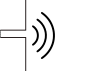
\includegraphics[width=0.55\textwidth]{lips_b}%
        \end{column}
    \end{columns}
        \pause
        \begin{flalign*}
            & \mathcal{P}_N(l_N, z) = Z_L(z) \mathcal{U}_N(l_N, z) &&
        \end{flalign*}
    \end{frame}

    \begin{frame}[t]{Сигнал от реч - модел на тръбите}
    \begin{columns}[T]
        \begin{column}{0.48\textwidth}
            {\tiny \begin{flalign*}
                & u_k(x, t) = \Q{u_k^+\B{t - \frac{x}{c}} - u_k^-\B{t + \frac{x}{c}}} && \\
                & p_k(x, t) = \cfrac{\rho c}{A_k}\Q{u_k^+\B{t - \frac{x}{c}} + u_k^-\B{t + \frac{x}{c}}} &&\\
                & U_k^{+}(z) = \cfrac{ z^{1/2}}{1 + r_k} U_{k+1}^{+}(z) - \cfrac{r_k z^{1/2}}{1+r_k} U_{k+1}^{-}(z) && \\
                & U_k^{-}(z) = - \cfrac{r_k z^{-1/2} }{1+r_k} U_{k+1}^{+}(z) + \cfrac{ z^{-1/2} }{1 + r_k} U_{k+1}^{-}(z)&&
            \end{flalign*}}
        \end{column}%
        \hfill%
        \begin{column}{0.24\textwidth}
        \end{column}%
        \hfill%
        \begin{column}{0.24\textwidth}
        \end{column}%
    \end{columns}
    \centering{Огрнаничения при устните}
    \begin{columns}[T]
        \begin{column}{0.48\textwidth}
            
\includegraphics[width=0.55\textwidth]{lips_a}%
        \end{column}
        \hfill
        \begin{column}{0.48\textwidth}
            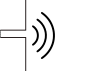
\includegraphics[width=0.55\textwidth]{lips_b}%
        \end{column}
    \end{columns}
        \begin{flalign*}
            & \mathcal{P}_N(l_N, z) = Z_L \mathcal{U}_N(l_N, z) &&
        \end{flalign*}
    \end{frame}

    \begin{frame}[t]{Сигнал от реч - модел на тръбите}
    \begin{columns}[T]
        \begin{column}{0.48\textwidth}
            {\tiny \begin{flalign*}
                & u_k(x, t) = \Q{u_k^+\B{t - \frac{x}{c}} - u_k^-\B{t + \frac{x}{c}}} && \\
                & p_k(x, t) = \cfrac{\rho c}{A_k}\Q{u_k^+\B{t - \frac{x}{c}} + u_k^-\B{t + \frac{x}{c}}} &&\\
                & U_k^{+}(z) = \cfrac{ z^{1/2}}{1 + r_k} U_{k+1}^{+}(z) - \cfrac{r_k z^{1/2}}{1+r_k} U_{k+1}^{-}(z) && \\
                & U_k^{-}(z) = - \cfrac{r_k z^{-1/2} }{1+r_k} U_{k+1}^{+}(z) + \cfrac{ z^{-1/2} }{1 + r_k} U_{k+1}^{-}(z)&&
            \end{flalign*}}
        \end{column}%
        \hfill%
        \begin{column}{0.24\textwidth}
        \end{column}%
        \hfill%
        \begin{column}{0.24\textwidth}
        \end{column}%
    \end{columns}
    \centering{Огрнаничения при устните}
    \begin{columns}[T]
        \begin{column}{0.48\textwidth}
            
\includegraphics[width=0.55\textwidth]{lips_a}%
        \end{column}
        \hfill
        \begin{column}{0.48\textwidth}
            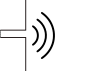
\includegraphics[width=0.55\textwidth]{lips_b}%
        \end{column}
    \end{columns}
        \begin{flalign*}
            & \mathcal{P}_N(l_N, z) = Z_L \mathcal{U}_N(l_N, z) \qquad p(l_N, t) \xleftrightarrow{\mathcal{F}\mathcal{S}}  \mathcal{P}_N(l_N, z), u_N(l_N, t) \xleftrightarrow{\mathcal{F}\mathcal{S}} \mathcal{U}_N(l_N, z)&&
        \end{flalign*}
    \end{frame}

    \begin{frame}[t]{Сигнал от реч - модел на тръбите}
    \begin{columns}[T]
        \begin{column}{0.48\textwidth}
            {\tiny \begin{flalign*}
                & {\color{mypink} u_k(x, t) = \Q{u_k^+\B{t - \frac{x}{c}} - u_k^-\B{t + \frac{x}{c}}}} && \\
                & {\color{mypink} p_k(x, t) = \cfrac{\rho c}{A_k}\Q{u_k^+\B{t - \frac{x}{c}} + u_k^-\B{t + \frac{x}{c}}}} &&\\
                & U_k^{+}(z) = \cfrac{ z^{1/2}}{1 + r_k} U_{k+1}^{+}(z) - \cfrac{r_k z^{1/2}}{1+r_k} U_{k+1}^{-}(z) && \\
                & U_k^{-}(z) = - \cfrac{r_k z^{-1/2} }{1+r_k} U_{k+1}^{+}(z) + \cfrac{ z^{-1/2} }{1 + r_k} U_{k+1}^{-}(z)&&
            \end{flalign*}}
        \end{column}%
        \hfill%
        \begin{column}{0.24\textwidth}
        \end{column}%
        \hfill%
        \begin{column}{0.24\textwidth}
        \end{column}%
    \end{columns}
    \centering{Огрнаничения при устните}
    \begin{columns}[T]
        \begin{column}{0.48\textwidth}
            
\includegraphics[width=0.55\textwidth]{lips_a}%
        \end{column}
        \hfill
        \begin{column}{0.48\textwidth}
            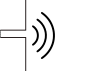
\includegraphics[width=0.55\textwidth]{lips_b}%
        \end{column}
    \end{columns}
        \begin{flalign*}
            & p_N(l_N, t) = Z_L u_N(l_N, t) &&
        \end{flalign*}
    \end{frame}

    \begin{frame}[t]{Сигнал от реч - модел на тръбите}
    \begin{columns}[T]
        \begin{column}{0.48\textwidth}
            {\tiny \begin{flalign*}
                & {\color{mypink} u_k(x, t) = \Q{u_k^+\B{t - \frac{x}{c}} - u_k^-\B{t + \frac{x}{c}}}} && \\
                & {\color{mypink} p_k(x, t) = \cfrac{\rho c}{A_k}\Q{u_k^+\B{t - \frac{x}{c}} + u_k^-\B{t + \frac{x}{c}}}} &&\\
                & U_k^{+}(z) = \cfrac{ z^{1/2}}{1 + r_k} U_{k+1}^{+}(z) - \cfrac{r_k z^{1/2}}{1+r_k} U_{k+1}^{-}(z) && \\
                & U_k^{-}(z) = - \cfrac{r_k z^{-1/2} }{1+r_k} U_{k+1}^{+}(z) + \cfrac{ z^{-1/2} }{1 + r_k} U_{k+1}^{-}(z)&&
            \end{flalign*}}
        \end{column}%
        \hfill%
        \begin{column}{0.24\textwidth}
        \end{column}%
        \hfill%
        \begin{column}{0.24\textwidth}
        \end{column}%
    \end{columns}
    \centering{Огрнаничения при устните}
    \begin{columns}[T]
        \begin{column}{0.48\textwidth}
            
\includegraphics[width=0.55\textwidth]{lips_a}%
        \end{column}
        \hfill
        \begin{column}{0.48\textwidth}
            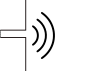
\includegraphics[width=0.55\textwidth]{lips_b}%
        \end{column}
    \end{columns}
        \begin{flalign*}
            & p_N(l_N, t) = Z_L u_N(l_N, t) &&\\
            &  u_N^{-}(t + \tau_N) \cfrac{(\rho c + A_N Z_L)}{A_N} = u_N^{+}(t - \tau_N) \cfrac{(A_N Z_L - \rho c)}{A_N} &&
        \end{flalign*}
    \end{frame}

    \begin{frame}[t]{Сигнал от реч - модел на тръбите}
    \begin{columns}[T]
        \begin{column}{0.48\textwidth}
            {\tiny \begin{flalign*}
                & {\color{mypink} u_k(x, t) = \Q{u_k^+\B{t - \frac{x}{c}} - u_k^-\B{t + \frac{x}{c}}}} && \\
                & {\color{mypink} p_k(x, t) = \cfrac{\rho c}{A_k}\Q{u_k^+\B{t - \frac{x}{c}} + u_k^-\B{t + \frac{x}{c}}}} &&\\
                & U_k^{+}(z) = \cfrac{ z^{1/2}}{1 + r_k} U_{k+1}^{+}(z) - \cfrac{r_k z^{1/2}}{1+r_k} U_{k+1}^{-}(z) && \\
                & U_k^{-}(z) = - \cfrac{r_k z^{-1/2} }{1+r_k} U_{k+1}^{+}(z) + \cfrac{ z^{-1/2} }{1 + r_k} U_{k+1}^{-}(z)&&
            \end{flalign*}}
        \end{column}%
        \hfill%
        \begin{column}{0.24\textwidth}
        \end{column}%
        \hfill%
        \begin{column}{0.24\textwidth}
        \end{column}%
    \end{columns}
    \centering{Огрнаничения при устните}
    \begin{columns}[T]
        \begin{column}{0.48\textwidth}
            
\includegraphics[width=0.55\textwidth]{lips_a}%
        \end{column}
        \hfill
        \begin{column}{0.48\textwidth}
            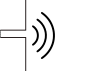
\includegraphics[width=0.55\textwidth]{lips_b}%
        \end{column}
    \end{columns}
        \begin{flalign*}
            & p_N(l_N, t) = Z_L u_N(l_N, t) &&\\
            &  u_N^{-}(t + \tau_N) \cfrac{(\rho c + A_N Z_L)}{A_N} = u_N^{+}(t - \tau_N) \cfrac{(A_N Z_L - \rho c)}{A_N} \qquad r_L = \cfrac{\frac{\rho c}{Z_L} - A_N}{\frac{\rho c}{Z_L} + A_N}&&
        \end{flalign*}
    \end{frame}

    \begin{frame}[t]{Сигнал от реч - модел на тръбите}
    \begin{columns}[T]
        \begin{column}{0.48\textwidth}
            {\tiny \begin{flalign*}
                & {\color{mypink} u_k(x, t) = \Q{u_k^+\B{t - \frac{x}{c}} - u_k^-\B{t + \frac{x}{c}}}} && \\
                & {\color{mypink} p_k(x, t) = \cfrac{\rho c}{A_k}\Q{u_k^+\B{t - \frac{x}{c}} + u_k^-\B{t + \frac{x}{c}}}} &&\\
                & U_k^{+}(z) = \cfrac{ z^{1/2}}{1 + r_k} U_{k+1}^{+}(z) - \cfrac{r_k z^{1/2}}{1+r_k} U_{k+1}^{-}(z) && \\
                & U_k^{-}(z) = - \cfrac{r_k z^{-1/2} }{1+r_k} U_{k+1}^{+}(z) + \cfrac{ z^{-1/2} }{1 + r_k} U_{k+1}^{-}(z)&&
            \end{flalign*}}
        \end{column}%
        \hfill%
        \begin{column}{0.24\textwidth}
        \end{column}%
        \hfill%
        \begin{column}{0.24\textwidth}
        \end{column}%
    \end{columns}
    \centering{Огрнаничения при устните}
    \begin{columns}[T]
        \begin{column}{0.48\textwidth}
            
\includegraphics[width=0.55\textwidth]{lips_a}%
        \end{column}
        \hfill
        \begin{column}{0.48\textwidth}
            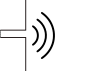
\includegraphics[width=0.55\textwidth]{lips_b}%
        \end{column}
    \end{columns}
        \begin{flalign*}
            & p_N(l_N, t) = Z_L u_N(l_N, t) &&\\
            &  u_N^{-}(t + \tau_N) = -r_L u_N^{+}(t - \tau_N) \qquad r_L = \cfrac{\frac{\rho c}{Z_L} - A_N}{\frac{\rho c}{Z_L} + A_N}&&
        \end{flalign*}
    \end{frame}

    \begin{frame}[t]{Сигнал от реч - модел на тръбите}
    \begin{columns}[T]
        \begin{column}{0.48\textwidth}
            {\tiny \begin{flalign*}
                & {\color{mypink} u_k(x, t) = \Q{u_k^+\B{t - \frac{x}{c}} - u_k^-\B{t + \frac{x}{c}}}} && \\
                & {\color{mypink} p_k(x, t) = \cfrac{\rho c}{A_k}\Q{u_k^+\B{t - \frac{x}{c}} + u_k^-\B{t + \frac{x}{c}}}} &&\\
                & U_k^{+}(z) = \cfrac{ z^{1/2}}{1 + r_k} U_{k+1}^{+}(z) - \cfrac{r_k z^{1/2}}{1+r_k} U_{k+1}^{-}(z) && \\
                & U_k^{-}(z) = - \cfrac{r_k z^{-1/2} }{1+r_k} U_{k+1}^{+}(z) + \cfrac{ z^{-1/2} }{1 + r_k} U_{k+1}^{-}(z)&&
            \end{flalign*}}
        \end{column}%
        \hfill%
        \begin{column}{0.24\textwidth}
            {\tiny \begin{flalign*}
                & r_L = \cfrac{\frac{\rho c}{Z_L} - A_N}{\frac{\rho c}{Z_L} + A_N} &&
            \end{flalign*}}
        \end{column}%
        \hfill%
        \begin{column}{0.24\textwidth}
        \end{column}%
    \end{columns}
    \centering{Огрнаничения при устните}
    \begin{columns}[T]
        \begin{column}{0.48\textwidth}
            
\includegraphics[width=0.55\textwidth]{lips_a}%
        \end{column}
        \hfill
        \begin{column}{0.48\textwidth}
            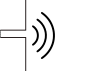
\includegraphics[width=0.55\textwidth]{lips_b}%
        \end{column}
    \end{columns}
    \begin{flalign*}
        & p_N(l_N, t) = Z_L u_N(l_N, t) &&\\
        &  u_N^{-}(t + \tau_N) = -r_L u_N^{+}(t - \tau_N) \qquad r_L = \cfrac{\frac{\rho c}{Z_L} - A_N}{\frac{\rho c}{Z_L} + A_N}&&
    \end{flalign*}
    \end{frame}

    \begin{frame}[t]{Сигнал от реч - модел на тръбите}
    \begin{columns}[T]
        \begin{column}{0.48\textwidth}
            {\tiny \begin{flalign*}
                & u_k(x, t) = \Q{u_k^+\B{t - \frac{x}{c}} - u_k^-\B{t + \frac{x}{c}}} && \\
                & p_k(x, t) = \cfrac{\rho c}{A_k}\Q{u_k^+\B{t - \frac{x}{c}} + u_k^-\B{t + \frac{x}{c}}} &&\\
                & U_k^{+}(z) = \cfrac{ z^{1/2}}{1 + r_k} U_{k+1}^{+}(z) - \cfrac{r_k z^{1/2}}{1+r_k} U_{k+1}^{-}(z) && \\
                & U_k^{-}(z) = - \cfrac{r_k z^{-1/2} }{1+r_k} U_{k+1}^{+}(z) + \cfrac{ z^{-1/2} }{1 + r_k} U_{k+1}^{-}(z)&&
            \end{flalign*}}
        \end{column}%
        \hfill%
        \begin{column}{0.14\textwidth}
            {\tiny \begin{flalign*}
                & r_L = \cfrac{\frac{\rho c}{Z_L} - A_N}{\frac{\rho c}{Z_L} + A_N} &&
            \end{flalign*}}
        \end{column}%
        \hfill%
        \begin{column}{0.34\textwidth}
        \end{column}%
    \end{columns}
    \pause
    \centering{Огрнаничения при глотиса}
    \pause
    {\small \begin{flalign*}
        & U_1(0, z) =  U_G(z) - \frac{P_1(0, z)}{Z_G(z)} &&\\
    \end{flalign*}}
    \end{frame}

    \begin{frame}[t]{Сигнал от реч - модел на тръбите}
    \begin{columns}[T]
        \begin{column}{0.48\textwidth}
            {\tiny \begin{flalign*}
                & u_k(x, t) = \Q{u_k^+\B{t - \frac{x}{c}} - u_k^-\B{t + \frac{x}{c}}} && \\
                & p_k(x, t) = \cfrac{\rho c}{A_k}\Q{u_k^+\B{t - \frac{x}{c}} + u_k^-\B{t + \frac{x}{c}}} &&\\
                & U_k^{+}(z) = \cfrac{ z^{1/2}}{1 + r_k} U_{k+1}^{+}(z) - \cfrac{r_k z^{1/2}}{1+r_k} U_{k+1}^{-}(z) && \\
                & U_k^{-}(z) = - \cfrac{r_k z^{-1/2} }{1+r_k} U_{k+1}^{+}(z) + \cfrac{ z^{-1/2} }{1 + r_k} U_{k+1}^{-}(z)&&
            \end{flalign*}}
        \end{column}%
        \hfill%
        \begin{column}{0.14\textwidth}
            {\tiny \begin{flalign*}
                & r_L = \cfrac{\frac{\rho c}{Z_L} - A_N}{\frac{\rho c}{Z_L} + A_N} &&
            \end{flalign*}}
        \end{column}%
        \hfill%
        \begin{column}{0.34\textwidth}
        \end{column}%
    \end{columns}
    \centering{Огрнаничения при глотиса}
    {\small \begin{flalign*}
        & U_1(0, z) =  U_G(z) - \frac{P_1(0, z)}{Z_G} &&\\
    \end{flalign*}}
    \end{frame}

    \begin{frame}[t]{Сигнал от реч - модел на тръбите}
    \begin{columns}[T]
        \begin{column}{0.48\textwidth}
            {\tiny \begin{flalign*}
                & u_k(x, t) = \Q{u_k^+\B{t - \frac{x}{c}} - u_k^-\B{t + \frac{x}{c}}} && \\
                & p_k(x, t) = \cfrac{\rho c}{A_k}\Q{u_k^+\B{t - \frac{x}{c}} + u_k^-\B{t + \frac{x}{c}}} &&\\
                & U_k^{+}(z) = \cfrac{ z^{1/2}}{1 + r_k} U_{k+1}^{+}(z) - \cfrac{r_k z^{1/2}}{1+r_k} U_{k+1}^{-}(z) && \\
                & U_k^{-}(z) = - \cfrac{r_k z^{-1/2} }{1+r_k} U_{k+1}^{+}(z) + \cfrac{ z^{-1/2} }{1 + r_k} U_{k+1}^{-}(z)&&
            \end{flalign*}}
        \end{column}%
        \hfill%
        \begin{column}{0.14\textwidth}
            {\tiny \begin{flalign*}
                & r_L = \cfrac{\frac{\rho c}{Z_L} - A_N}{\frac{\rho c}{Z_L} + A_N} &&
            \end{flalign*}}
        \end{column}%
        \hfill%
        \begin{column}{0.34\textwidth}
        \end{column}%
    \end{columns}
    \centering{Огрнаничения при глотиса}
    {\small \begin{flalign*}
        & U_1(0, z) =  U_G(z) - \frac{P_1(0, z)}{Z_G} && \\
        & u_1(0, t) \xleftrightarrow{\mathcal{F}\mathcal{S}} U_1(0, z), u_G(t) \xleftrightarrow{\mathcal{F}\mathcal{S}} U_G(z), p_1(0, t) \xleftrightarrow{\mathcal{F}\mathcal{S}} P_1(0, z) &&\\
    \end{flalign*}}
    \end{frame}

    \begin{frame}[t]{Сигнал от реч - модел на тръбите}
    \begin{columns}[T]
        \begin{column}{0.48\textwidth}
            {\tiny \begin{flalign*}
                & u_k(x, t) = \Q{u_k^+\B{t - \frac{x}{c}} - u_k^-\B{t + \frac{x}{c}}} && \\
                & p_k(x, t) = \cfrac{\rho c}{A_k}\Q{u_k^+\B{t - \frac{x}{c}} + u_k^-\B{t + \frac{x}{c}}} &&\\
                & U_k^{+}(z) = \cfrac{ z^{1/2}}{1 + r_k} U_{k+1}^{+}(z) - \cfrac{r_k z^{1/2}}{1+r_k} U_{k+1}^{-}(z) && \\
                & U_k^{-}(z) = - \cfrac{r_k z^{-1/2} }{1+r_k} U_{k+1}^{+}(z) + \cfrac{ z^{-1/2} }{1 + r_k} U_{k+1}^{-}(z)&&
            \end{flalign*}}
        \end{column}%
        \hfill%
        \begin{column}{0.14\textwidth}
            {\tiny \begin{flalign*}
                & r_L = \cfrac{\frac{\rho c}{Z_L} - A_N}{\frac{\rho c}{Z_L} + A_N} &&
            \end{flalign*}}
        \end{column}%
        \hfill%
        \begin{column}{0.34\textwidth}
        \end{column}%
    \end{columns}
    \centering{Огрнаничения при глотиса}
    {\small \begin{flalign*}
        & U_1(0, z) =  U_G(z) - \frac{P_1(0, z)}{Z_G} && \\
        & u_1(0, t) \xleftrightarrow{\mathcal{F}\mathcal{S}} U_1(0, z), u_G(t) \xleftrightarrow{\mathcal{F}\mathcal{S}} U_G(z), p_1(0, t) \xleftrightarrow{\mathcal{F}\mathcal{S}} P_1(0, z) &&\\
        & u_1(0, t) = u_G(t) - \frac{p_1(0, t)}{Z_G}&&
    \end{flalign*}}
    \end{frame}

    \begin{frame}[t]{Сигнал от реч - модел на тръбите}
    \begin{columns}[T]
        \begin{column}{0.48\textwidth}
            {\tiny \begin{flalign*}
                & {\color{mypink} u_k(x, t) = \Q{u_k^+\B{t - \frac{x}{c}} - u_k^-\B{t + \frac{x}{c}}}} && \\
                & {\color{mypink} p_k(x, t) = \cfrac{\rho c}{A_k}\Q{u_k^+\B{t - \frac{x}{c}} + u_k^-\B{t + \frac{x}{c}}}} &&\\
                & U_k^{+}(z) = \cfrac{ z^{1/2}}{1 + r_k} U_{k+1}^{+}(z) - \cfrac{r_k z^{1/2}}{1+r_k} U_{k+1}^{-}(z) && \\
                & U_k^{-}(z) = - \cfrac{r_k z^{-1/2} }{1+r_k} U_{k+1}^{+}(z) + \cfrac{ z^{-1/2} }{1 + r_k} U_{k+1}^{-}(z)&&
            \end{flalign*}}
        \end{column}%
        \hfill%
        \begin{column}{0.14\textwidth}
            {\tiny \begin{flalign*}
                & r_L = \cfrac{\frac{\rho c}{Z_L} - A_N}{\frac{\rho c}{Z_L} + A_N} &&
            \end{flalign*}}
        \end{column}%
        \hfill%
        \begin{column}{0.34\textwidth}
        \end{column}%
    \end{columns}
    \centering{Огрнаничения при глотиса}
    {\small \begin{flalign*}
        & U_1(0, z) =  U_G(z) - \frac{P_1(0, z)}{Z_G} && \\
        & u_1(0, t) \xleftrightarrow{\mathcal{F}\mathcal{S}} U_1(0, z), u_G(t) \xleftrightarrow{\mathcal{F}\mathcal{S}} U_G(z), p_1(0, t) \xleftrightarrow{\mathcal{F}\mathcal{S}} P_1(0, z) &&\\
        & u_1(0, t) = u_G(t) - \frac{p_1(0, t)}{Z_G}&&
    \end{flalign*}}
    \end{frame}

    \begin{frame}[t]{Сигнал от реч - модел на тръбите}
    \begin{columns}[T]
        \begin{column}{0.48\textwidth}
            {\tiny \begin{flalign*}
                & {\color{mypink} u_k(x, t) = \Q{u_k^+\B{t - \frac{x}{c}} - u_k^-\B{t + \frac{x}{c}}}} && \\
                & {\color{mypink} p_k(x, t) = \cfrac{\rho c}{A_k}\Q{u_k^+\B{t - \frac{x}{c}} + u_k^-\B{t + \frac{x}{c}}}} &&\\
                & U_k^{+}(z) = \cfrac{ z^{1/2}}{1 + r_k} U_{k+1}^{+}(z) - \cfrac{r_k z^{1/2}}{1+r_k} U_{k+1}^{-}(z) && \\
                & U_k^{-}(z) = - \cfrac{r_k z^{-1/2} }{1+r_k} U_{k+1}^{+}(z) + \cfrac{ z^{-1/2} }{1 + r_k} U_{k+1}^{-}(z)&&
            \end{flalign*}}
        \end{column}%
        \hfill%
        \begin{column}{0.14\textwidth}
            {\tiny \begin{flalign*}
                & r_L = \cfrac{\frac{\rho c}{Z_L} - A_N}{\frac{\rho c}{Z_L} + A_N} &&
            \end{flalign*}}
        \end{column}%
        \hfill%
        \begin{column}{0.34\textwidth}
        \end{column}%
    \end{columns}
    \centering{Огрнаничения при глотиса}
    {\small \begin{flalign*}
        & U_1(0, z) =  U_G(z) - \frac{P_1(0, z)}{Z_G} && \\
        & u_1(0, t) \xleftrightarrow{\mathcal{F}\mathcal{S}} U_1(0, z), u_G(t) \xleftrightarrow{\mathcal{F}\mathcal{S}} U_G(z), p_1(0, t) \xleftrightarrow{\mathcal{F}\mathcal{S}} P_1(0, z) &&\\
        & u_1(0, t) = u_G(t) - \frac{p_1(0, t)}{Z_G}&& \\
        & u_1^{+}(t) = u_G(t)\Q{\frac{A_1 Z_G}{A_1 Z_G + \rho  c}} + u_1^{-}(t)\Q{\frac{A_1 Z_G - \rho  c}{A_1 Z_G + \rho  c}} &&
    \end{flalign*}}
    \end{frame}

    \begin{frame}[t]{Сигнал от реч - модел на тръбите}
    \begin{columns}[T]
        \begin{column}{0.48\textwidth}
            {\tiny \begin{flalign*}
                & u_k(x, t) = \Q{u_k^+\B{t - \frac{x}{c}} - u_k^-\B{t + \frac{x}{c}}} && \\
                & p_k(x, t) = \cfrac{\rho c}{A_k}\Q{u_k^+\B{t - \frac{x}{c}} + u_k^-\B{t + \frac{x}{c}}} &&\\
                & U_k^{+}(z) = \cfrac{ z^{1/2}}{1 + r_k} U_{k+1}^{+}(z) - \cfrac{r_k z^{1/2}}{1+r_k} U_{k+1}^{-}(z) && \\
                & U_k^{-}(z) = - \cfrac{r_k z^{-1/2} }{1+r_k} U_{k+1}^{+}(z) + \cfrac{ z^{-1/2} }{1 + r_k} U_{k+1}^{-}(z)&&
            \end{flalign*}}
        \end{column}%
        \hfill%
        \begin{column}{0.14\textwidth}
            {\tiny \begin{flalign*}
                & r_L = \cfrac{\frac{\rho c}{Z_L} - A_N}{\frac{\rho c}{Z_L} + A_N} &&
            \end{flalign*}}
        \end{column}%
        \hfill%
        \begin{column}{0.34\textwidth}
        \end{column}%
    \end{columns}
    \centering{Огрнаничения при глотиса}
    {\small \begin{flalign*}
        & U_1(0, z) =  U_G(z) - \frac{P_1(0, z)}{Z_G} && \\
        & u_1(0, t) \xleftrightarrow{\mathcal{F}\mathcal{S}} U_1(0, z), u_G(t) \xleftrightarrow{\mathcal{F}\mathcal{S}} U_G(z), p_1(0, t) \xleftrightarrow{\mathcal{F}\mathcal{S}} P_1(0, z) &&\\
        & u_1(0, t) = u_G(t) - \frac{p_1(0, t)}{Z_G}&& \\
        & u_1^{+}(t) = u_G(t)\Q{\frac{A_1 Z_G}{A_1 Z_G + \rho  c}} + u_1^{-}(t)\Q{\frac{A_1 Z_G - \rho  c}{A_1 Z_G + \rho  c}} \qquad r_G = \B{\cfrac{A_1 Z_G - \rho c}{A_1 Z_G + \rho c}}&&
    \end{flalign*}}
    \end{frame}


    \begin{frame}[t]{Сигнал от реч - модел на тръбите}
    \begin{columns}[T]
        \begin{column}{0.48\textwidth}
            {\tiny \begin{flalign*}
                & u_k(x, t) = \Q{u_k^+\B{t - \frac{x}{c}} - u_k^-\B{t + \frac{x}{c}}} && \\
                & p_k(x, t) = \cfrac{\rho c}{A_k}\Q{u_k^+\B{t - \frac{x}{c}} + u_k^-\B{t + \frac{x}{c}}} &&\\
                & U_k^{+}(z) = \cfrac{ z^{1/2}}{1 + r_k} U_{k+1}^{+}(z) - \cfrac{r_k z^{1/2}}{1+r_k} U_{k+1}^{-}(z) && \\
                & U_k^{-}(z) = - \cfrac{r_k z^{-1/2} }{1+r_k} U_{k+1}^{+}(z) + \cfrac{ z^{-1/2} }{1 + r_k} U_{k+1}^{-}(z)&&
            \end{flalign*}}
        \end{column}%
        \hfill%
        \begin{column}{0.14\textwidth}
            {\tiny \begin{flalign*}
                & r_L = \cfrac{\frac{\rho c}{Z_L} - A_N}{\frac{\rho c}{Z_L} + A_N} &&
            \end{flalign*}}
        \end{column}%
        \hfill%
        \begin{column}{0.34\textwidth}
        \end{column}%
    \end{columns}
    \centering{Огрнаничения при глотиса}
    {\small \begin{flalign*}
        & U_1(0, z) =  U_G(z) - \frac{P_1(0, z)}{Z_G} && \\
        & u_1(0, t) \xleftrightarrow{\mathcal{F}\mathcal{S}} U_1(0, z), u_G(t) \xleftrightarrow{\mathcal{F}\mathcal{S}} U_G(z), p_1(0, t) \xleftrightarrow{\mathcal{F}\mathcal{S}} P_1(0, z) &&\\
        & u_1(0, t) = u_G(t) - \frac{p_1(0, t)}{Z_G}&& \\
        & u_1^{+}(t) = u_G(t) \Q{\frac{1 + r_G}{2}} + r_G u_1^{-}(t) \qquad r_G = \B{\cfrac{A_1 Z_G - \rho c}{A_1 Z_G + \rho c}}&&
    \end{flalign*}}
    \end{frame}

    \begin{frame}[t]{Сигнал от реч - модел на тръбите}
    \begin{columns}[T]
        \begin{column}{0.48\textwidth}
            {\tiny \begin{flalign*}
                & u_k(x, t) = \Q{u_k^+\B{t - \frac{x}{c}} - u_k^-\B{t + \frac{x}{c}}} && \\
                & p_k(x, t) = \cfrac{\rho c}{A_k}\Q{u_k^+\B{t - \frac{x}{c}} + u_k^-\B{t + \frac{x}{c}}} &&\\
                & U_k^{+}(z) = \cfrac{ z^{1/2}}{1 + r_k} U_{k+1}^{+}(z) - \cfrac{r_k z^{1/2}}{1+r_k} U_{k+1}^{-}(z) && \\
                & U_k^{-}(z) = - \cfrac{r_k z^{-1/2} }{1+r_k} U_{k+1}^{+}(z) + \cfrac{ z^{-1/2} }{1 + r_k} U_{k+1}^{-}(z)&&
            \end{flalign*}}
        \end{column}%
        \hfill%
        \begin{column}{0.14\textwidth}
            {\tiny \begin{flalign*}
                & r_L = \cfrac{\frac{\rho c}{Z_L} - A_N}{\frac{\rho c}{Z_L} + A_N} &&
            \end{flalign*}}
        \end{column}%
        \hfill%
        \begin{column}{0.34\textwidth}
        \end{column}%
    \end{columns}
    \centering{Огрнаничения при глотиса}
    {\small \begin{flalign*}
        & U_1(0, z) =  U_G(z) - \frac{P_1(0, z)}{Z_G} && \\
        & u_1(0, t) \xleftrightarrow{\mathcal{F}\mathcal{S}} U_1(0, z), u_G(t) \xleftrightarrow{\mathcal{F}\mathcal{S}} U_G(z), p_1(0, t) \xleftrightarrow{\mathcal{F}\mathcal{S}} P_1(0, z) &&\\
        & u_1(0, t) = u_G(t) - \frac{p_1(0, t)}{Z_G}&& \\
        & u_1^{+}(t) = u_G(t) \Q{\frac{1 + r_G}{2}} + r_G u_1^{-}(t) \qquad r_G = \B{\cfrac{A_1 Z_G - \rho c}{A_1 Z_G + \rho c}}&&\\
        & U_1^{+}(z) = U_G(z) \Q{\frac{1 + r_G}{2}} + r_G U_1^{-}(z) &&
    \end{flalign*}}
    \end{frame}

    \begin{frame}[t]{Сигнал от реч - модел на тръбите}
    \begin{columns}[T]
        \begin{column}{0.48\textwidth}
            {\tiny \begin{flalign*}
                & u_k(x, t) = \Q{u_k^+\B{t - \frac{x}{c}} - u_k^-\B{t + \frac{x}{c}}} && \\
                & p_k(x, t) = \cfrac{\rho c}{A_k}\Q{u_k^+\B{t - \frac{x}{c}} + u_k^-\B{t + \frac{x}{c}}} &&\\
                & U_k^{+}(z) = \cfrac{ z^{1/2}}{1 + r_k} U_{k+1}^{+}(z) - \cfrac{r_k z^{1/2}}{1+r_k} U_{k+1}^{-}(z) && \\
                & U_k^{-}(z) = - \cfrac{r_k z^{-1/2} }{1+r_k} U_{k+1}^{+}(z) + \cfrac{ z^{-1/2} }{1 + r_k} U_{k+1}^{-}(z)&&
            \end{flalign*}}
        \end{column}%
        \hfill%
        \begin{column}{0.14\textwidth}
            {\tiny \begin{flalign*}
                & r_L = \cfrac{\frac{\rho c}{Z_L} - A_N}{\frac{\rho c}{Z_L} + A_N} &&
            \end{flalign*}}
        \end{column}%
        \hfill%
        \begin{column}{0.34\textwidth}
            {\tiny \begin{flalign*}
                & r_G = \B{\cfrac{A_1 Z_G - \rho c}{A_1 Z_G + \rho c}} &&\\
                & U_1^{+}(z) = U_G(z) \Q{\frac{1 + r_G}{2}} + r_G U_1^{-}(z) &&
            \end{flalign*}}
        \end{column}%
    \end{columns}
    \centering{Огрнаничения при глотиса}
    {\small \begin{flalign*}
        & U_1(0, z) =  U_G(z) - \frac{P_1(0, z)}{Z_G} && \\
        & u_1(0, t) \xleftrightarrow{\mathcal{F}\mathcal{S}} U_1(0, z), u_G(t) \xleftrightarrow{\mathcal{F}\mathcal{S}} U_G(z), p_1(0, t) \xleftrightarrow{\mathcal{F}\mathcal{S}} P_1(0, z) &&\\
        & u_1(0, t) = u_G(t) - \frac{p_1(0, t)}{Z_G}&& \\
        & u_1^{+}(t) = u_G(t) \Q{\frac{1 + r_G}{2}} + r_G u_1^{-}(t) \qquad r_G = \B{\cfrac{A_1 Z_G - \rho c}{A_1 Z_G + \rho c}}&&\\
        & U_1^{+}(z) = U_G(z) \Q{\frac{1 + r_G}{2}} + r_G U_1^{-}(z) &&
    \end{flalign*}}
    \end{frame}

    \begin{frame}[t]{Сигнал от реч - модел на тръбите}
    \begin{columns}[T]
        \begin{column}{0.48\textwidth}
            {\tiny \begin{flalign*}
                & u_k(x, t) = \Q{u_k^+\B{t - \frac{x}{c}} - u_k^-\B{t + \frac{x}{c}}} && \\
                & p_k(x, t) = \cfrac{\rho c}{A_k}\Q{u_k^+\B{t - \frac{x}{c}} + u_k^-\B{t + \frac{x}{c}}} &&\\
                & U_k^{+}(z) = \cfrac{ z^{1/2}}{1 + r_k} U_{k+1}^{+}(z) - \cfrac{r_k z^{1/2}}{1+r_k} U_{k+1}^{-}(z) && \\
                & U_k^{-}(z) = - \cfrac{r_k z^{-1/2} }{1+r_k} U_{k+1}^{+}(z) + \cfrac{ z^{-1/2} }{1 + r_k} U_{k+1}^{-}(z)&&
            \end{flalign*}}
        \end{column}%
        \hfill%
        \begin{column}{0.14\textwidth}
            {\tiny \begin{flalign*}
                & r_L = \cfrac{\frac{\rho c}{Z_L} - A_N}{\frac{\rho c}{Z_L} + A_N} &&
            \end{flalign*}}
        \end{column}%
        \hfill%
        \begin{column}{0.34\textwidth}
            {\tiny \begin{flalign*}
                & r_G = \B{\cfrac{A_1 Z_G - \rho c}{A_1 Z_G + \rho c}} &&\\
                & U_1^{+}(z) = U_G(z) \Q{\frac{1 + r_G}{2}} + r_G U_1^{-}(z) &&
            \end{flalign*}}
        \end{column}%
    \end{columns}
    \end{frame}

    \begin{frame}[t]{Сигнал от реч - модел на тръбите}
    \begin{columns}[T]
        \begin{column}{0.48\textwidth}
            {\tiny \begin{flalign*}
                & U_k^{+}(z) = \cfrac{ z^{1/2}}{1 + r_k} U_{k+1}^{+}(z) - \cfrac{r_k z^{1/2}}{1+r_k} U_{k+1}^{-}(z) && \\
                & U_k^{-}(z) = - \cfrac{r_k z^{-1/2} }{1+r_k} U_{k+1}^{+}(z) + \cfrac{ z^{-1/2} }{1 + r_k} U_{k+1}^{-}(z)&&
            \end{flalign*}}
        \end{column}%
        \hfill%
        \begin{column}{0.14\textwidth}
            {\tiny \begin{flalign*}
                & r_L = \cfrac{\frac{\rho c}{Z_L} - A_N}{\frac{\rho c}{Z_L} + A_N} &&
            \end{flalign*}}
        \end{column}%
        \hfill%
        \begin{column}{0.34\textwidth}
            {\tiny \begin{flalign*}
                & r_G = \B{\cfrac{A_1 Z_G - \rho c}{A_1 Z_G + \rho c}} &&\\
                & U_1^{+}(z) = U_G(z) \Q{\frac{1 + r_G}{2}} + r_G U_1^{-}(z) &&
            \end{flalign*}}
        \end{column}%
    \end{columns}
    \pause
    \centering{Общ вид на $\mathcal{V}$}
    \pause
    \begin{columns}
        \begin{column}{0.48\textwidth}
            \begin{flalign*}
                & U_{N+1}^{+} (z) = U_L(z)\qquad \qquad \qquad \qquad \quad \qquad \quad &&
            \end{flalign*}
        \end{column}
        \hfill
        \begin{column}{0.48\textwidth}
        \end{column}
    \end{columns}
    \end{frame}

    \begin{frame}[t]{Сигнал от реч - модел на тръбите}
    \begin{columns}[T]
        \begin{column}{0.48\textwidth}
            {\tiny \begin{flalign*}
                & U_k^{+}(z) = \cfrac{ z^{1/2}}{1 + r_k} U_{k+1}^{+}(z) - \cfrac{r_k z^{1/2}}{1+r_k} U_{k+1}^{-}(z) && \\
                & U_k^{-}(z) = - \cfrac{r_k z^{-1/2} }{1+r_k} U_{k+1}^{+}(z) + \cfrac{ z^{-1/2} }{1 + r_k} U_{k+1}^{-}(z)&&
            \end{flalign*}}
        \end{column}%
        \hfill%
        \begin{column}{0.14\textwidth}
            {\tiny \begin{flalign*}
                & r_L = \cfrac{\frac{\rho c}{Z_L} - A_N}{\frac{\rho c}{Z_L} + A_N} &&
            \end{flalign*}}
        \end{column}%
        \hfill%
        \begin{column}{0.34\textwidth}
            {\tiny \begin{flalign*}
                & r_G = \B{\cfrac{A_1 Z_G - \rho c}{A_1 Z_G + \rho c}} &&\\
                & U_1^{+}(z) = U_G(z) \Q{\frac{1 + r_G}{2}} + r_G U_1^{-}(z) &&
            \end{flalign*}}
        \end{column}%
    \end{columns}
    \centering{Общ вид на $\mathcal{V}$}
    \begin{columns}
        \begin{column}{0.48\textwidth}
            \begin{flalign*}
                & U_{N+1}^{+} (z) = U_L(z)\qquad \qquad \qquad \qquad \quad \qquad \quad &&\\
                & U_{N+1}^{-}(z) = 0 &&
            \end{flalign*}
        \end{column}
        \hfill
        \begin{column}{0.48\textwidth}
        \end{column}
    \end{columns}
    \end{frame}

    \begin{frame}[t]{Сигнал от реч - модел на тръбите}
    \begin{columns}[T]
        \begin{column}{0.48\textwidth}
            {\tiny \begin{flalign*}
                & U_k^{+}(z) = \cfrac{ z^{1/2}}{1 + r_k} U_{k+1}^{+}(z) - \cfrac{r_k z^{1/2}}{1+r_k} U_{k+1}^{-}(z) && \\
                & U_k^{-}(z) = - \cfrac{r_k z^{-1/2} }{1+r_k} U_{k+1}^{+}(z) + \cfrac{ z^{-1/2} }{1 + r_k} U_{k+1}^{-}(z)&&
            \end{flalign*}}
        \end{column}%
        \hfill%
        \begin{column}{0.14\textwidth}
            {\tiny \begin{flalign*}
                & r_L = \cfrac{\frac{\rho c}{Z_L} - A_N}{\frac{\rho c}{Z_L} + A_N} &&
            \end{flalign*}}
        \end{column}%
        \hfill%
        \begin{column}{0.34\textwidth}
            {\tiny \begin{flalign*}
                & r_G = \B{\cfrac{A_1 Z_G - \rho c}{A_1 Z_G + \rho c}} &&\\
                & U_1^{+}(z) = U_G(z) \Q{\frac{1 + r_G}{2}} + r_G U_1^{-}(z) &&
            \end{flalign*}}
        \end{column}%
    \end{columns}
    \centering{Общ вид на $\mathcal{V}$}
    \begin{columns}
        \begin{column}{0.48\textwidth}
            \begin{flalign*}
                & U_{N+1}^{+} (z) = U_L(z)\qquad \qquad \qquad \qquad \quad \qquad \quad &&\\
                & U_{N+1}^{-}(z) = 0  \qquad r_N = r_L&&
            \end{flalign*}
        \end{column}
        \begin{column}{0.48\textwidth}
            \begin{flalign*}
            \end{flalign*}
        \end{column}
    \end{columns}
    \end{frame}

    \begin{frame}[t]{Сигнал от реч - модел на тръбите}
    \begin{columns}[T]
        \begin{column}{0.48\textwidth}
            {\tiny \begin{flalign*}
                & U_k^{+}(z) = \cfrac{ z^{1/2}}{1 + r_k} U_{k+1}^{+}(z) - \cfrac{r_k z^{1/2}}{1+r_k} U_{k+1}^{-}(z) && \\
                & U_k^{-}(z) = - \cfrac{r_k z^{-1/2} }{1+r_k} U_{k+1}^{+}(z) + \cfrac{ z^{-1/2} }{1 + r_k} U_{k+1}^{-}(z)&&
            \end{flalign*}}
        \end{column}%
        \hfill%
        \begin{column}{0.14\textwidth}
            {\tiny \begin{flalign*}
                & r_L = \cfrac{\frac{\rho c}{Z_L} - A_N}{\frac{\rho c}{Z_L} + A_N} &&
            \end{flalign*}}
        \end{column}%
        \hfill%
        \begin{column}{0.34\textwidth}
            {\tiny \begin{flalign*}
                & r_G = \B{\cfrac{A_1 Z_G - \rho c}{A_1 Z_G + \rho c}} &&\\
                & U_1^{+}(z) = U_G(z) \Q{\frac{1 + r_G}{2}} + r_G U_1^{-}(z) &&
            \end{flalign*}}
        \end{column}%
    \end{columns}
    \centering{Общ вид на $\mathcal{V}$}
    \begin{columns}
        \begin{column}{0.48\textwidth}
            \begin{flalign*}
                & U_{N+1}^{+} (z) = U_L(z)\qquad \qquad \qquad \qquad \quad \qquad \quad &&\\
                & U_{N+1}^{-}(z) = 0  \qquad r_N = r_L \rightarrow A_{N+1} = \cfrac{\rho c}{Z_L}&&
            \end{flalign*}
        \end{column}
        \begin{column}{0.48\textwidth}
            \begin{flalign*}
            \end{flalign*}
        \end{column}
    \end{columns}
    \end{frame}

    \begin{frame}[t]{Сигнал от реч - модел на тръбите}
    \begin{columns}[T]
        \begin{column}{0.48\textwidth}
            {\tiny \begin{flalign*}
                & U_k^{+}(z) = \cfrac{ z^{1/2}}{1 + r_k} U_{k+1}^{+}(z) - \cfrac{r_k z^{1/2}}{1+r_k} U_{k+1}^{-}(z) && \\
                & U_k^{-}(z) = - \cfrac{r_k z^{-1/2} }{1+r_k} U_{k+1}^{+}(z) + \cfrac{ z^{-1/2} }{1 + r_k} U_{k+1}^{-}(z)&&
            \end{flalign*}}
        \end{column}%
        \hfill%
        \begin{column}{0.14\textwidth}
            {\tiny \begin{flalign*}
                & r_L = \cfrac{\frac{\rho c}{Z_L} - A_N}{\frac{\rho c}{Z_L} + A_N} &&
            \end{flalign*}}
        \end{column}%
        \hfill%
        \begin{column}{0.34\textwidth}
            {\tiny \begin{flalign*}
                & r_G = \B{\cfrac{A_1 Z_G - \rho c}{A_1 Z_G + \rho c}} &&\\
                & U_1^{+}(z) = U_G(z) \Q{\frac{1 + r_G}{2}} + r_G U_1^{-}(z) &&
            \end{flalign*}}
        \end{column}%
    \end{columns}
    \centering{Общ вид на $\mathcal{V}$}
    \begin{columns}
        \begin{column}{0.48\textwidth}
            \begin{flalign*}
                & U_{N+1}^{+} (z) = U_L(z)\qquad \qquad \qquad \qquad \quad \qquad \quad &&\\
                & U_{N+1}^{-}(z) = 0 \qquad r_N = r_L \rightarrow A_{N+1} = \cfrac{\rho c}{Z_L} &&\\
                \\
                & U_k = Q_k U_{k+1}&&
            \end{flalign*}
        \end{column}
        \begin{column}{0.48\textwidth}
            \begin{flalign*}
            \end{flalign*}
        \end{column}
    \end{columns}  
    \end{frame}

    \begin{frame}[t]{Сигнал от реч - модел на тръбите}
    \begin{columns}[T]
        \begin{column}{0.48\textwidth}
            {\tiny \begin{flalign*}
                & U_k^{+}(z) = \cfrac{ z^{1/2}}{1 + r_k} U_{k+1}^{+}(z) - \cfrac{r_k z^{1/2}}{1+r_k} U_{k+1}^{-}(z) && \\
                & U_k^{-}(z) = - \cfrac{r_k z^{-1/2} }{1+r_k} U_{k+1}^{+}(z) + \cfrac{ z^{-1/2} }{1 + r_k} U_{k+1}^{-}(z)&&
            \end{flalign*}}
        \end{column}%
        \hfill%
        \begin{column}{0.14\textwidth}
            {\tiny \begin{flalign*}
                & r_L = \cfrac{\frac{\rho c}{Z_L} - A_N}{\frac{\rho c}{Z_L} + A_N} &&
            \end{flalign*}}
        \end{column}%
        \hfill%
        \begin{column}{0.34\textwidth}
            {\tiny \begin{flalign*}
                & r_G = \B{\cfrac{A_1 Z_G - \rho c}{A_1 Z_G + \rho c}} &&\\
                & U_1^{+}(z) = U_G(z) \Q{\frac{1 + r_G}{2}} + r_G U_1^{-}(z) &&
            \end{flalign*}}
        \end{column}%
    \end{columns}
    \centering{Общ вид на $\mathcal{V}$}
    \begin{columns}[T]
        \begin{column}{0.48\textwidth}
            \begin{flalign*}
                & U_{N+1}^{+} (z) = U_L(z)\qquad \qquad \qquad \qquad \quad \qquad \quad &&\\
                & U_{N+1}^{-}(z) = 0 \qquad r_N = r_L \rightarrow A_{N+1} = \cfrac{\rho c}{Z_L} &&\\
                \\
                & U_k = Q_k U_{k+1} &&\\
                & U_k = 
                \begin{bmatrix}
                    U_k^{+}(z) \\
                    U_k^{-}(z) \\
                \end{bmatrix}&&
            \end{flalign*}
        \end{column}
        \begin{column}{0.48\textwidth}
            \begin{flalign*}
                \\
                & Q_k = 
                \begin{bmatrix}
                    \cfrac{z^{1/2}}{1 + r_k} & \cfrac{-r_k z^{1/2}}{1 + r_k} \\
                    & \\
                    \cfrac{-r_k z^{-1/2}}{1 + r_k} & \cfrac{z^{-1/2}}{1 + r_k} \\
                \end{bmatrix}&&
            \end{flalign*}
        \end{column}
    \end{columns}   
    \end{frame}

    \begin{frame}[t]{Сигнал от реч - модел на тръбите}
    \begin{columns}[T]
        \begin{column}{0.48\textwidth}
            {\tiny \begin{flalign*}
                & U_k^{+}(z) = \cfrac{ z^{1/2}}{1 + r_k} U_{k+1}^{+}(z) - \cfrac{r_k z^{1/2}}{1+r_k} U_{k+1}^{-}(z) && \\
                & U_k^{-}(z) = - \cfrac{r_k z^{-1/2} }{1+r_k} U_{k+1}^{+}(z) + \cfrac{ z^{-1/2} }{1 + r_k} U_{k+1}^{-}(z)&&
            \end{flalign*}}
        \end{column}%
        \hfill%
        \begin{column}{0.14\textwidth}
            {\tiny \begin{flalign*}
                & r_L = \cfrac{\frac{\rho c}{Z_L} - A_N}{\frac{\rho c}{Z_L} + A_N} &&
            \end{flalign*}}
        \end{column}%
        \hfill%
        \begin{column}{0.34\textwidth}
            {\tiny \begin{flalign*}
                & r_G = \B{\cfrac{A_1 Z_G - \rho c}{A_1 Z_G + \rho c}} &&\\
                & U_1^{+}(z) = U_G(z) \Q{\frac{1 + r_G}{2}} + r_G U_1^{-}(z) &&
            \end{flalign*}}
        \end{column}%
    \end{columns}
    \centering{Общ вид на $\mathcal{V}$}
    \begin{columns}[T]
        \begin{column}{0.48\textwidth}
            \begin{flalign*}
                & U_{N+1}^{+} (z) = U_L(z) \qquad \qquad \qquad \qquad \quad \qquad \quad &&\\
                & U_{N+1}^{-}(z) = 0 \qquad r_N = r_L \rightarrow A_{N+1} = \cfrac{\rho c}{Z_L} &&\\
                \\
                & U_k = Q_k U_{k+1} &&\\
                & U_k = 
                \begin{bmatrix}
                    U_k^{+}(z) \\
                    U_k^{-}(z) \\
                \end{bmatrix} &&\\
                & \medmath{U_1 = }&&
            \end{flalign*}
        \end{column}
        \begin{column}{0.48\textwidth}
            \begin{flalign*}
                \\
                & Q_k = 
                \begin{bmatrix}
                    \cfrac{z^{1/2}}{1 + r_k} & \cfrac{-r_k z^{1/2}}{1 + r_k} \\
                    & \\
                    \cfrac{-r_k z^{-1/2}}{1 + r_k} & \cfrac{z^{-1/2}}{1 + r_k} \\
                \end{bmatrix}&&
            \end{flalign*}
        \end{column}
    \end{columns}   
    \end{frame}

    \begin{frame}[t]{Сигнал от реч - модел на тръбите}
        \begin{columns}[T]
            \begin{column}{0.48\textwidth}
                {\tiny \begin{flalign*}
                    & U_k^{+}(z) = \cfrac{ z^{1/2}}{1 + r_k} U_{k+1}^{+}(z) - \cfrac{r_k z^{1/2}}{1+r_k} U_{k+1}^{-}(z) && \\
                    & U_k^{-}(z) = - \cfrac{r_k z^{-1/2} }{1+r_k} U_{k+1}^{+}(z) + \cfrac{ z^{-1/2} }{1 + r_k} U_{k+1}^{-}(z)&&
                \end{flalign*}}
            \end{column}%
            \hfill%
            \begin{column}{0.14\textwidth}
                {\tiny \begin{flalign*}
                    & r_L = \cfrac{\frac{\rho c}{Z_L} - A_N}{\frac{\rho c}{Z_L} + A_N} &&
                \end{flalign*}}
            \end{column}%
            \hfill%
            \begin{column}{0.34\textwidth}
                {\tiny \begin{flalign*}
                    & r_G = \B{\cfrac{A_1 Z_G - \rho c}{A_1 Z_G + \rho c}} &&\\
                    & U_1^{+}(z) = U_G(z) \Q{\frac{1 + r_G}{2}} + r_G U_1^{-}(z) &&
                \end{flalign*}}
            \end{column}%
        \end{columns}
        \centering{Общ вид на $\mathcal{V}$}
        \begin{columns}[T]
            \begin{column}{0.48\textwidth}
                \begin{flalign*}
                    & U_{N+1}^{+} (z) = U_L(z) \qquad \qquad \qquad \qquad \quad \qquad \quad &&\\
                    & U_{N+1}^{-}(z) = 0 \qquad r_N = r_L \rightarrow A_{N+1} = \cfrac{\rho c}{Z_L} &&\\
                    \\
                    & U_k = Q_k U_{k+1} &&\\
                    & U_k = 
                    \begin{bmatrix}
                        U_k^{+}(z) \\
                        U_k^{-}(z) \\
                    \end{bmatrix} &&\\
                    & \medmath{U_1 = Q_1 U_2}&&
                \end{flalign*}
            \end{column}
            \begin{column}{0.48\textwidth}
                \begin{flalign*}
                    \\
                    & Q_k = 
                    \begin{bmatrix}
                        \cfrac{z^{1/2}}{1 + r_k} & \cfrac{-r_k z^{1/2}}{1 + r_k} \\
                        & \\
                        \cfrac{-r_k z^{-1/2}}{1 + r_k} & \cfrac{z^{-1/2}}{1 + r_k} \\
                    \end{bmatrix}&&\\
                \end{flalign*}
            \end{column}
        \end{columns}   
    \end{frame}

    \begin{frame}[t]{Сигнал от реч - модел на тръбите}
    \begin{columns}[T]
        \begin{column}{0.48\textwidth}
            {\tiny \begin{flalign*}
                & U_k^{+}(z) = \cfrac{ z^{1/2}}{1 + r_k} U_{k+1}^{+}(z) - \cfrac{r_k z^{1/2}}{1+r_k} U_{k+1}^{-}(z) && \\
                & U_k^{-}(z) = - \cfrac{r_k z^{-1/2} }{1+r_k} U_{k+1}^{+}(z) + \cfrac{ z^{-1/2} }{1 + r_k} U_{k+1}^{-}(z)&&
            \end{flalign*}}
        \end{column}%
        \hfill%
        \begin{column}{0.14\textwidth}
            {\tiny \begin{flalign*}
                & r_L = \cfrac{\frac{\rho c}{Z_L} - A_N}{\frac{\rho c}{Z_L} + A_N} &&
            \end{flalign*}}
        \end{column}%
        \hfill%
        \begin{column}{0.34\textwidth}
            {\tiny \begin{flalign*}
                & r_G = \B{\cfrac{A_1 Z_G - \rho c}{A_1 Z_G + \rho c}} &&\\
                & U_1^{+}(z) = U_G(z) \Q{\frac{1 + r_G}{2}} + r_G U_1^{-}(z) &&
            \end{flalign*}}
        \end{column}%
    \end{columns}
    \centering{Общ вид на $\mathcal{V}$}
    \begin{columns}[T]
        \begin{column}{0.48\textwidth}
            \begin{flalign*}
                & U_{N+1}^{+} (z) = U_L(z) \qquad \qquad \qquad \qquad \quad \qquad \quad &&\\
                & U_{N+1}^{-}(z) = 0 \qquad r_N = r_L \rightarrow A_{N+1} = \cfrac{\rho c}{Z_L} &&\\
                \\
                & U_k = Q_k U_{k+1} &&\\
                & U_k = 
                \begin{bmatrix}
                    U_k^{+}(z) \\
                    U_k^{-}(z) \\
                \end{bmatrix} &&\\
                & \medmath{U_1 = Q_1 U_2 = Q_1 Q_2 U_3}&&
            \end{flalign*}
        \end{column}
        \begin{column}{0.48\textwidth}
            \begin{flalign*}
                \\
                & Q_k = 
                \begin{bmatrix}
                    \cfrac{z^{1/2}}{1 + r_k} & \cfrac{-r_k z^{1/2}}{1 + r_k} \\
                    & \\
                    \cfrac{-r_k z^{-1/2}}{1 + r_k} & \cfrac{z^{-1/2}}{1 + r_k} \\
                \end{bmatrix}&&
            \end{flalign*}
        \end{column}
    \end{columns}   
    \end{frame}

    \begin{frame}[t]{Сигнал от реч - модел на тръбите}
    \begin{columns}[T]
        \begin{column}{0.48\textwidth}
            {\tiny \begin{flalign*}
                & U_k^{+}(z) = \cfrac{ z^{1/2}}{1 + r_k} U_{k+1}^{+}(z) - \cfrac{r_k z^{1/2}}{1+r_k} U_{k+1}^{-}(z) && \\
                & U_k^{-}(z) = - \cfrac{r_k z^{-1/2} }{1+r_k} U_{k+1}^{+}(z) + \cfrac{ z^{-1/2} }{1 + r_k} U_{k+1}^{-}(z)&&
            \end{flalign*}}
        \end{column}%
        \hfill%
        \begin{column}{0.14\textwidth}
            {\tiny \begin{flalign*}
                & r_L = \cfrac{\frac{\rho c}{Z_L} - A_N}{\frac{\rho c}{Z_L} + A_N} &&
            \end{flalign*}}
        \end{column}%
        \hfill%
        \begin{column}{0.34\textwidth}
            {\tiny \begin{flalign*}
                & r_G = \B{\cfrac{A_1 Z_G - \rho c}{A_1 Z_G + \rho c}} &&\\
                & U_1^{+}(z) = U_G(z) \Q{\frac{1 + r_G}{2}} + r_G U_1^{-}(z) &&
            \end{flalign*}}
        \end{column}%
    \end{columns}
    \centering{Общ вид на $\mathcal{V}$}
    \begin{columns}[T]
        \begin{column}{0.48\textwidth}
            \begin{flalign*}
                & U_{N+1}^{+} (z) = U_L(z) \qquad \qquad \qquad \qquad \quad \qquad \quad &&\\
                & U_{N+1}^{-}(z) = 0 \qquad r_N = r_L \rightarrow A_{N+1} = \cfrac{\rho c}{Z_L} &&\\
                \\
                & U_k = Q_k U_{k+1} &&\\
                & U_k = 
                \begin{bmatrix}
                    U_k^{+}(z) \\
                    U_k^{-}(z) \\
                \end{bmatrix} &&\\
                & \medmath{U_1 = Q_1 U_2 = Q_1 Q_2 U_3 = \ldots = \Q{\prod_{i = 1}^N Q_i} U_{N+1}} &&
            \end{flalign*}
        \end{column}
        \begin{column}{0.48\textwidth}
            \begin{flalign*}
                \\
                & Q_k = 
                \begin{bmatrix}
                    \cfrac{z^{1/2}}{1 + r_k} & \cfrac{-r_k z^{1/2}}{1 + r_k} \\
                    & \\
                    \cfrac{-r_k z^{-1/2}}{1 + r_k} & \cfrac{z^{-1/2}}{1 + r_k} \\
                \end{bmatrix}&&
            \end{flalign*}
        \end{column}
    \end{columns}   
    \end{frame}


    \begin{frame}[t]{Сигнал от реч - модел на тръбите}
    \begin{columns}[T]
        \begin{column}{0.48\textwidth}
            {\tiny \begin{flalign*}
                & U_k^{+}(z) = \cfrac{ z^{1/2}}{1 + r_k} U_{k+1}^{+}(z) - \cfrac{r_k z^{1/2}}{1+r_k} U_{k+1}^{-}(z) && \\
                & U_k^{-}(z) = - \cfrac{r_k z^{-1/2} }{1+r_k} U_{k+1}^{+}(z) + \cfrac{ z^{-1/2} }{1 + r_k} U_{k+1}^{-}(z)&&
            \end{flalign*}}
        \end{column}%
        \hfill%
        \begin{column}{0.14\textwidth}
            {\tiny \begin{flalign*}
                & r_L = \cfrac{\frac{\rho c}{Z_L} - A_N}{\frac{\rho c}{Z_L} + A_N} &&
            \end{flalign*}}
        \end{column}%
        \hfill%
        \begin{column}{0.34\textwidth}
            {\tiny \begin{flalign*}
                & r_G = \B{\cfrac{A_1 Z_G - \rho c}{A_1 Z_G + \rho c}} &&\\
                & U_1^{+}(z) = U_G(z) \Q{\frac{1 + r_G}{2}} + r_G U_1^{-}(z) &&
            \end{flalign*}}
        \end{column}%
    \end{columns}
    \centering{Общ вид на $\mathcal{V}$}
    \begin{columns}[b]
        \begin{column}{0.48\textwidth}
            \begin{flalign*}
                & U_{N+1}^{+} (z) = U_L(z)  \qquad \qquad \qquad \qquad \quad \qquad \quad &&\\
                & U_{N+1}^{-}(z) = 0 \qquad r_N = r_L \rightarrow A_{N+1} = \cfrac{\rho c}{Z_L} &&\\
                \\
                & U_k = Q_k U_{k+1} &&\\
                & U_k = 
                \begin{bmatrix}
                    U_k^{+}(z) \\
                    U_k^{-}(z) \\
                \end{bmatrix} &&\\
                & \medmath{U_1 = Q_1 U_2 = Q_1 Q_2 U_3 = \ldots = \Q{\prod_{i = 1}^N Q_i} U_{N+1}} &&
            \end{flalign*}
            \vspace{0pt}
        \end{column}
        \begin{column}{0.48\textwidth}
            \begin{flalign*}
                & Q_k = 
                \begin{bmatrix}
                    \cfrac{z^{1/2}}{1 + r_k} & \cfrac{-r_k z^{1/2}}{1 + r_k} \\
                    & \\
                    \cfrac{-r_k z^{-1/2}}{1 + r_k} & \cfrac{z^{-1/2}}{1 + r_k} \\
                \end{bmatrix} && \\
                \\
                &  \medmath{= \Q{\prod_{i = 1}^N Q_i}\begin{bmatrix}
                    U_{N+1}^{+}(z) \\
                    U_{N+1}^{-}(z) \\
                \end{bmatrix}}&&
            \end{flalign*}
            \vspace{0pt}
        \end{column}
    \end{columns}   
    \end{frame}

    \begin{frame}[t]{Сигнал от реч - модел на тръбите}
    \begin{columns}[T]
        \begin{column}{0.48\textwidth}
            {\tiny \begin{flalign*}
                & U_k^{+}(z) = \cfrac{ z^{1/2}}{1 + r_k} U_{k+1}^{+}(z) - \cfrac{r_k z^{1/2}}{1+r_k} U_{k+1}^{-}(z) && \\
                & U_k^{-}(z) = - \cfrac{r_k z^{-1/2} }{1+r_k} U_{k+1}^{+}(z) + \cfrac{ z^{-1/2} }{1 + r_k} U_{k+1}^{-}(z)&&
            \end{flalign*}}
        \end{column}%
        \hfill%
        \begin{column}{0.14\textwidth}
            {\tiny \begin{flalign*}
                & r_L = \cfrac{\frac{\rho c}{Z_L} - A_N}{\frac{\rho c}{Z_L} + A_N} &&
            \end{flalign*}}
        \end{column}%
        \hfill%
        \begin{column}{0.34\textwidth}
            {\tiny \begin{flalign*}
                & r_G = \B{\cfrac{A_1 Z_G - \rho c}{A_1 Z_G + \rho c}} &&\\
                & U_1^{+}(z) = U_G(z) \Q{\frac{1 + r_G}{2}} + r_G U_1^{-}(z) &&
            \end{flalign*}}
        \end{column}%
    \end{columns}
    \centering{Общ вид на $\mathcal{V}$}
    \begin{columns}[b]
        \begin{column}{0.48\textwidth}
            \begin{flalign*}
                & U_{N+1}^{+} (z) = U_L(z)  &&\\
                & U_{N+1}^{-}(z) = 0 \qquad r_N = r_L \rightarrow A_{N+1} = \cfrac{\rho c}{Z_L} &&\\
                \\
                & U_k = Q_k U_{k+1} &&\\
                & U_k = 
                \begin{bmatrix}
                    U_k^{+}(z) \\
                    U_k^{-}(z) \\
                \end{bmatrix} &&\\
                & \medmath{U_1 = Q_1 U_2 = Q_1 Q_2 U_3 = \ldots = \Q{\prod_{i = 1}^N Q_i} U_{N+1}} &&
            \end{flalign*}
            \vspace{0pt}
        \end{column}
        \begin{column}{0.48\textwidth}
            \begin{flalign*}
                & Q_k = 
                \begin{bmatrix}
                    \cfrac{z^{1/2}}{1 + r_k} & \cfrac{-r_k z^{1/2}}{1 + r_k} \\
                    & \\
                    \cfrac{-r_k z^{-1/2}}{1 + r_k} & \cfrac{z^{-1/2}}{1 + r_k} \\
                \end{bmatrix}&& \\
                \\
                &  \medmath{= \Q{\prod_{i = 1}^N Q_i}\begin{bmatrix}
                    U_{N+1}^{+}(z) \\
                    U_{N+1}^{-}(z) \\
                \end{bmatrix} = \Q{\prod_{i = 1}^N Q_i}\begin{bmatrix}
                    U_L(z) \\
                    0 \\
                \end{bmatrix}}&& 
            \end{flalign*}
            \vspace{0pt}
        \end{column}
    \end{columns}   
    \end{frame}

    \begin{frame}[t]{Сигнал от реч - модел на тръбите}
    \begin{columns}[T]
        \begin{column}{0.48\textwidth}
            {\tiny \begin{flalign*}
                & U_k^{+}(z) = \cfrac{ z^{1/2}}{1 + r_k} U_{k+1}^{+}(z) - \cfrac{r_k z^{1/2}}{1+r_k} U_{k+1}^{-}(z) && \\
                & U_k^{-}(z) = - \cfrac{r_k z^{-1/2} }{1+r_k} U_{k+1}^{+}(z) + \cfrac{ z^{-1/2} }{1 + r_k} U_{k+1}^{-}(z)&&
            \end{flalign*}}
        \end{column}%
        \hfill%
        \begin{column}{0.14\textwidth}
            {\tiny \begin{flalign*}
                & r_L = \cfrac{\frac{\rho c}{Z_L} - A_N}{\frac{\rho c}{Z_L} + A_N} &&
            \end{flalign*}}
        \end{column}%
        \hfill%
        \begin{column}{0.34\textwidth}
            {\tiny \begin{flalign*}
                & r_G = \B{\cfrac{A_1 Z_G - \rho c}{A_1 Z_G + \rho c}} &&\\
                & U_1^{+}(z) = U_G(z) \Q{\frac{1 + r_G}{2}} + r_G U_1^{-}(z) &&
            \end{flalign*}}
        \end{column}%
    \end{columns}
    \centering{Общ вид на $\mathcal{V}$}
    \begin{columns}[c, onlytextwidth]
        \begin{column}{0.30\textwidth}
        \begin{flalign*}
            & Q_k = 
                \begin{bmatrix}
                    \cfrac{z^{1/2}}{1 + r_k} & \cfrac{-r_k z^{1/2}}{1 + r_k} \\
                    & \\
                    \cfrac{-r_k z^{-1/2}}{1 + r_k} & \cfrac{z^{-1/2}}{1 + r_k} \\
                \end{bmatrix}&&
        \end{flalign*}
        \end{column}
        \begin{column}{0.70\textwidth}
            \begin{flalign*}
                & U_1 = \Q{\prod_{i = 1}^N Q_i}\begin{bmatrix}
                    U_L(z) \\
                    0 \\
                \end{bmatrix} &&
            \end{flalign*}
        \end{column}
        \hfill
    \end{columns}   
    \end{frame}

    \begin{frame}[t]{Сигнал от реч - модел на тръбите}
    \begin{columns}[T]
        \begin{column}{0.48\textwidth}
            {\tiny \begin{flalign*}
                & U_k^{+}(z) = \cfrac{ z^{1/2}}{1 + r_k} U_{k+1}^{+}(z) - \cfrac{r_k z^{1/2}}{1+r_k} U_{k+1}^{-}(z) && \\
                & U_k^{-}(z) = - \cfrac{r_k z^{-1/2} }{1+r_k} U_{k+1}^{+}(z) + \cfrac{ z^{-1/2} }{1 + r_k} U_{k+1}^{-}(z)&&
            \end{flalign*}}
        \end{column}%
        \hfill%
        \begin{column}{0.14\textwidth}
            {\tiny \begin{flalign*}
                & r_L = \cfrac{\frac{\rho c}{Z_L} - A_N}{\frac{\rho c}{Z_L} + A_N} &&
            \end{flalign*}}
        \end{column}%
        \hfill%
        \begin{column}{0.34\textwidth}
            {\tiny \begin{flalign*}
                & r_G = \B{\cfrac{A_1 Z_G - \rho c}{A_1 Z_G + \rho c}} &&\\
                & U_1^{+}(z) = U_G(z) \Q{\frac{1 + r_G}{2}} + r_G U_1^{-}(z) &&
            \end{flalign*}}
        \end{column}%
    \end{columns}
    \centering{Общ вид на $\mathcal{V}$}
    \begin{columns}[c, onlytextwidth]
        \begin{column}{0.30\textwidth}
        \begin{flalign*}
            & Q_k = 
                \begin{bmatrix}
                    \cfrac{z^{1/2}}{1 + r_k} & \cfrac{-r_k z^{1/2}}{1 + r_k} \\
                    & \\
                    \cfrac{-r_k z^{-1/2}}{1 + r_k} & \cfrac{z^{-1/2}}{1 + r_k} \\
                \end{bmatrix}&&
        \end{flalign*}
        \end{column}
        \begin{column}{0.70\textwidth}
            \begin{flalign*}
                & U_1 = \Q{\prod_{i = 1}^N Q_i}\begin{bmatrix}
                    1 \\
                    0 \\
                \end{bmatrix}U_L(z) &&
            \end{flalign*}
        \end{column}
        \hfill
    \end{columns}   
    \end{frame}

    \begin{frame}[t]{Сигнал от реч - модел на тръбите}
    \begin{columns}[T]
        \begin{column}{0.48\textwidth}
            {\tiny \begin{flalign*}
                & U_k^{+}(z) = \cfrac{ z^{1/2}}{1 + r_k} U_{k+1}^{+}(z) - \cfrac{r_k z^{1/2}}{1+r_k} U_{k+1}^{-}(z) && \\
                & U_k^{-}(z) = - \cfrac{r_k z^{-1/2} }{1+r_k} U_{k+1}^{+}(z) + \cfrac{ z^{-1/2} }{1 + r_k} U_{k+1}^{-}(z)&&
            \end{flalign*}}
        \end{column}%
        \hfill%
        \begin{column}{0.14\textwidth}
            {\tiny \begin{flalign*}
                & r_L = \cfrac{\frac{\rho c}{Z_L} - A_N}{\frac{\rho c}{Z_L} + A_N} &&
            \end{flalign*}}
        \end{column}%
        \hfill%
        \begin{column}{0.34\textwidth}
            {\tiny \begin{flalign*}
                & r_G = \B{\cfrac{A_1 Z_G - \rho c}{A_1 Z_G + \rho c}} &&\\
                & U_1^{+}(z) = U_G(z) \Q{\frac{1 + r_G}{2}} + r_G U_1^{-}(z) &&
            \end{flalign*}}
        \end{column}%
    \end{columns}
    \centering{Общ вид на $\mathcal{V}$}
    \begin{columns}[c, onlytextwidth]
        \begin{column}{0.30\textwidth}
        \begin{flalign*}
            & Q_k = 
                \begin{bmatrix}
                    \cfrac{z^{1/2}}{1 + r_k} & \cfrac{-r_k z^{1/2}}{1 + r_k} \\
                    & \\
                    \cfrac{-r_k z^{-1/2}}{1 + r_k} & \cfrac{z^{-1/2}}{1 + r_k} \\
                \end{bmatrix}&&
        \end{flalign*}
        \end{column}
        \begin{column}{0.70\textwidth}
            \begin{flalign*}
                & U_1 = \Q{\prod_{i = 1}^N Q_i}\begin{bmatrix}
                    1 \\
                    0 \\
                \end{bmatrix}U_L(z) &&
            \end{flalign*}
        \end{column}
        \hfill
    \end{columns}
    \begin{flalign*}
        &U_G(z) =  &&
    \end{flalign*}
    \end{frame}

    \begin{frame}[t]{Сигнал от реч - модел на тръбите}
    \begin{columns}[T]
        \begin{column}{0.48\textwidth}
            {\tiny \begin{flalign*}
                & U_k^{+}(z) = \cfrac{ z^{1/2}}{1 + r_k} U_{k+1}^{+}(z) - \cfrac{r_k z^{1/2}}{1+r_k} U_{k+1}^{-}(z) && \\
                & U_k^{-}(z) = - \cfrac{r_k z^{-1/2} }{1+r_k} U_{k+1}^{+}(z) + \cfrac{ z^{-1/2} }{1 + r_k} U_{k+1}^{-}(z)&&
            \end{flalign*}}
        \end{column}%
        \hfill%
        \begin{column}{0.14\textwidth}
            {\tiny \begin{flalign*}
                & r_L = \cfrac{\frac{\rho c}{Z_L} - A_N}{\frac{\rho c}{Z_L} + A_N} &&
            \end{flalign*}}
        \end{column}%
        \hfill%
        \begin{column}{0.34\textwidth}
            {\tiny \begin{flalign*}
                & r_G = \B{\cfrac{A_1 Z_G - \rho c}{A_1 Z_G + \rho c}} &&\\
                & U_1^{+}(z) = U_G(z) \Q{\frac{1 + r_G}{2}} + r_G U_1^{-}(z) &&
            \end{flalign*}}
        \end{column}%
    \end{columns}
    \centering{Общ вид на $\mathcal{V}$}
    \begin{columns}[c, onlytextwidth]
        \begin{column}{0.30\textwidth}
        \begin{flalign*}
            & Q_k = 
                \begin{bmatrix}
                    \cfrac{z^{1/2}}{1 + r_k} & \cfrac{-r_k z^{1/2}}{1 + r_k} \\
                    & \\
                    \cfrac{-r_k z^{-1/2}}{1 + r_k} & \cfrac{z^{-1/2}}{1 + r_k} \\
                \end{bmatrix}&&
        \end{flalign*}
        \end{column}
        \begin{column}{0.70\textwidth}
            \begin{flalign*}
                & U_1 = \Q{\prod_{i = 1}^N Q_i}\begin{bmatrix}
                    1 \\
                    0 \\
                \end{bmatrix}U_L(z) &&
            \end{flalign*}
        \end{column}
        \hfill
    \end{columns}   
    \begin{flalign*}
        &U_G(z) =  \Q{\cfrac{2}{1 + r_G}, -\cfrac{2r_G}{1 + r_G}}U_1&&
    \end{flalign*}
    \end{frame}

    \begin{frame}[t]{Сигнал от реч - модел на тръбите}
    \begin{columns}[T]
        \begin{column}{0.48\textwidth}
            {\tiny \begin{flalign*}
                & U_k^{+}(z) = \cfrac{ z^{1/2}}{1 + r_k} U_{k+1}^{+}(z) - \cfrac{r_k z^{1/2}}{1+r_k} U_{k+1}^{-}(z) && \\
                & U_k^{-}(z) = - \cfrac{r_k z^{-1/2} }{1+r_k} U_{k+1}^{+}(z) + \cfrac{ z^{-1/2} }{1 + r_k} U_{k+1}^{-}(z)&&
            \end{flalign*}}
        \end{column}%
        \hfill%
        \begin{column}{0.14\textwidth}
            {\tiny \begin{flalign*}
                & r_L = \cfrac{\frac{\rho c}{Z_L} - A_N}{\frac{\rho c}{Z_L} + A_N} &&
            \end{flalign*}}
        \end{column}%
        \hfill%
        \begin{column}{0.34\textwidth}
            {\tiny \begin{flalign*}
                & r_G = \B{\cfrac{A_1 Z_G - \rho c}{A_1 Z_G + \rho c}} &&\\
                & U_1^{+}(z) = U_G(z) \Q{\frac{1 + r_G}{2}} + r_G U_1^{-}(z) &&
            \end{flalign*}}
        \end{column}%
    \end{columns}
    \centering{Общ вид на $\mathcal{V}$}
    \begin{columns}[c, onlytextwidth]
        \begin{column}{0.30\textwidth}
        \begin{flalign*}
            & Q_k = 
                \begin{bmatrix}
                    \cfrac{z^{1/2}}{1 + r_k} & \cfrac{-r_k z^{1/2}}{1 + r_k} \\
                    & \\
                    \cfrac{-r_k z^{-1/2}}{1 + r_k} & \cfrac{z^{-1/2}}{1 + r_k} \\
                \end{bmatrix}&&
        \end{flalign*}
        \end{column}
        \begin{column}{0.70\textwidth}
            \begin{flalign*}
                & U_1 = \Q{\prod_{i = 1}^N Q_i}\begin{bmatrix}
                    1 \\
                    0 \\
                \end{bmatrix}U_L(z) &&
            \end{flalign*}
        \end{column}
        \hfill
    \end{columns}   
    \begin{flalign*}
        &U_G(z) =  \Q{\cfrac{2}{1 + r_G}, -\cfrac{2r_G}{1 + r_G}}U_1 = \Q{\cfrac{2}{1 + r_G}, -\cfrac{2r_G}{1 + r_G}}\Q{\prod_{i = 1}^N Q_i}\begin{bmatrix}
            1 \\
            0 \\
        \end{bmatrix}U_L(z)&&
    \end{flalign*}
    \end{frame}

    \begin{frame}[t]{Сигнал от реч - модел на тръбите}
    \begin{columns}[T]
        \begin{column}{0.48\textwidth}
            {\tiny \begin{flalign*}
                & U_k^{+}(z) = \cfrac{ z^{1/2}}{1 + r_k} U_{k+1}^{+}(z) - \cfrac{r_k z^{1/2}}{1+r_k} U_{k+1}^{-}(z) && \\
                & U_k^{-}(z) = - \cfrac{r_k z^{-1/2} }{1+r_k} U_{k+1}^{+}(z) + \cfrac{ z^{-1/2} }{1 + r_k} U_{k+1}^{-}(z)&&
            \end{flalign*}}
        \end{column}%
        \hfill%
        \begin{column}{0.14\textwidth}
            {\tiny \begin{flalign*}
                & r_L = \cfrac{\frac{\rho c}{Z_L} - A_N}{\frac{\rho c}{Z_L} + A_N} &&
            \end{flalign*}}
        \end{column}%
        \hfill%
        \begin{column}{0.34\textwidth}
            {\tiny \begin{flalign*}
                & r_G = \B{\cfrac{A_1 Z_G - \rho c}{A_1 Z_G + \rho c}} &&\\
                & U_1^{+}(z) = U_G(z) \Q{\frac{1 + r_G}{2}} + r_G U_1^{-}(z) &&
            \end{flalign*}}
        \end{column}%
    \end{columns}
    \centering{Общ вид на $\mathcal{V}$}
    \begin{columns}[c, onlytextwidth]
        \begin{column}{0.30\textwidth}
        \begin{flalign*}
            & Q_k = 
                \begin{bmatrix}
                    \cfrac{z^{1/2}}{1 + r_k} & \cfrac{-r_k z^{1/2}}{1 + r_k} \\
                    & \\
                    \cfrac{-r_k z^{-1/2}}{1 + r_k} & \cfrac{z^{-1/2}}{1 + r_k} \\
                \end{bmatrix}&&
        \end{flalign*}
        \end{column}
        \begin{column}{0.70\textwidth}
            \begin{flalign*}
                & &U_G(z) =  \Q{\cfrac{2}{1 + r_G}, -\cfrac{2r_G}{1 + r_G}}\Q{\prod_{i = 1}^N Q_i}\begin{bmatrix}
                    1 \\
                    0 \\
                \end{bmatrix}U_L(z) &&
            \end{flalign*}
        \end{column}
        \hfill
    \end{columns}
    \end{frame}

    \begin{frame}[t]{Сигнал от реч - модел на тръбите}
    \begin{columns}[T]
        \begin{column}{0.48\textwidth}
            {\tiny \begin{flalign*}
                & U_k^{+}(z) = \cfrac{ z^{1/2}}{1 + r_k} U_{k+1}^{+}(z) - \cfrac{r_k z^{1/2}}{1+r_k} U_{k+1}^{-}(z) && \\
                & U_k^{-}(z) = - \cfrac{r_k z^{-1/2} }{1+r_k} U_{k+1}^{+}(z) + \cfrac{ z^{-1/2} }{1 + r_k} U_{k+1}^{-}(z)&&
            \end{flalign*}}
        \end{column}%
        \hfill%
        \begin{column}{0.14\textwidth}
            {\tiny \begin{flalign*}
                & r_L = \cfrac{\frac{\rho c}{Z_L} - A_N}{\frac{\rho c}{Z_L} + A_N} &&
            \end{flalign*}}
        \end{column}%
        \hfill%
        \begin{column}{0.34\textwidth}
            {\tiny \begin{flalign*}
                & r_G = \B{\cfrac{A_1 Z_G - \rho c}{A_1 Z_G + \rho c}} &&\\
                & U_1^{+}(z) = U_G(z) \Q{\frac{1 + r_G}{2}} + r_G U_1^{-}(z) &&
            \end{flalign*}}
        \end{column}%
    \end{columns}
    \centering{Общ вид на $\mathcal{V}$}
    \begin{columns}[c, onlytextwidth]
        \begin{column}{0.30\textwidth}
        \begin{flalign*}
            & Q_k = 
                \begin{bmatrix}
                    \cfrac{z^{1/2}}{1 + r_k} & \cfrac{-r_k z^{1/2}}{1 + r_k} \\
                    & \\
                    \cfrac{-r_k z^{-1/2}}{1 + r_k} & \cfrac{z^{-1/2}}{1 + r_k} \\
                \end{bmatrix}&&
        \end{flalign*}
        \end{column}
        \begin{column}{0.70\textwidth}
            \begin{flalign*}
                & &U_G(z) =  \Q{\cfrac{2}{1 + r_G}, -\cfrac{2r_G}{1 + r_G}}\Q{\prod_{i = 1}^N Q_i}\begin{bmatrix}
                    1 \\
                    0 \\
                \end{bmatrix}U_L(z) &&
            \end{flalign*}
        \end{column}
        \hfill
    \end{columns}
    \begin{flalign*}
        & Q_k = 
            \begin{bmatrix}
                \cfrac{z^{1/2}}{1 + r_k} & \cfrac{-r_k z^{1/2}}{1 + r_k} \\
                & \\
                \cfrac{-r_k z^{-1/2}}{1 + r_k} & \cfrac{z^{-1/2}}{1 + r_k} \\
            \end{bmatrix}&&
    \end{flalign*}
    \end{frame}

    \begin{frame}[t]{Сигнал от реч - модел на тръбите}
    \begin{columns}[T]
        \begin{column}{0.48\textwidth}
            {\tiny \begin{flalign*}
                & U_k^{+}(z) = \cfrac{ z^{1/2}}{1 + r_k} U_{k+1}^{+}(z) - \cfrac{r_k z^{1/2}}{1+r_k} U_{k+1}^{-}(z) && \\
                & U_k^{-}(z) = - \cfrac{r_k z^{-1/2} }{1+r_k} U_{k+1}^{+}(z) + \cfrac{ z^{-1/2} }{1 + r_k} U_{k+1}^{-}(z)&&
            \end{flalign*}}
        \end{column}%
        \hfill%
        \begin{column}{0.14\textwidth}
            {\tiny \begin{flalign*}
                & r_L = \cfrac{\frac{\rho c}{Z_L} - A_N}{\frac{\rho c}{Z_L} + A_N} &&
            \end{flalign*}}
        \end{column}%
        \hfill%
        \begin{column}{0.34\textwidth}
            {\tiny \begin{flalign*}
                & r_G = \B{\cfrac{A_1 Z_G - \rho c}{A_1 Z_G + \rho c}} &&\\
                & U_1^{+}(z) = U_G(z) \Q{\frac{1 + r_G}{2}} + r_G U_1^{-}(z) &&
            \end{flalign*}}
        \end{column}%
    \end{columns}
    \centering{Общ вид на $\mathcal{V}$}
    \begin{columns}[c, onlytextwidth]
        \begin{column}{0.30\textwidth}
        \begin{flalign*}
            & Q_k = 
                \begin{bmatrix}
                    \cfrac{z^{1/2}}{1 + r_k} & \cfrac{-r_k z^{1/2}}{1 + r_k} \\
                    & \\
                    \cfrac{-r_k z^{-1/2}}{1 + r_k} & \cfrac{z^{-1/2}}{1 + r_k} \\
                \end{bmatrix}&&
        \end{flalign*}
        \end{column}
        \begin{column}{0.70\textwidth}
            \begin{flalign*}
                & &U_G(z) =  \Q{\cfrac{2}{1 + r_G}, -\cfrac{2r_G}{1 + r_G}}\Q{\prod_{i = 1}^N Q_i}\begin{bmatrix}
                    1 \\
                    0 \\
                \end{bmatrix}U_L(z) &&
            \end{flalign*}
        \end{column}
        \hfill
    \end{columns}
    \begin{flalign*}
        & Q_k = \left[\begin{array}{cc}
                \cfrac{z^{1/2}}{1 + r_k} & \cfrac{-r_k z^{1/2}}{1 + r_k} \\
                & \\
                \cfrac{-r_k z^{-1/2}}{1 + r_k} & \cfrac{z^{-1/2}}{1 + r_k} \\
            \end{array}\right] = 
            z^{1/2}\left[\begin{array}{cc}
                \cfrac{1}{1 + r_k} & \cfrac{-r_k}{1 + r_k} \\
                & \\
                \cfrac{-r_k z^{-1}}{1 + r_k} & \cfrac{z^{-1}}{1 + r_k} \\
            \end{array}\right] = 
            z^{1/2} \widehat{Q}_k && 
    \end{flalign*}
    \end{frame}

    \begin{frame}[t]{Сигнал от реч - модел на тръбите}
    \begin{columns}[T]
        \begin{column}{0.48\textwidth}
            {\tiny \begin{flalign*}
                & U_k^{+}(z) = \cfrac{ z^{1/2}}{1 + r_k} U_{k+1}^{+}(z) - \cfrac{r_k z^{1/2}}{1+r_k} U_{k+1}^{-}(z) && \\
                & U_k^{-}(z) = - \cfrac{r_k z^{-1/2} }{1+r_k} U_{k+1}^{+}(z) + \cfrac{ z^{-1/2} }{1 + r_k} U_{k+1}^{-}(z)&&
            \end{flalign*}}
        \end{column}%
        \hfill%
        \begin{column}{0.14\textwidth}
            {\tiny \begin{flalign*}
                & r_L = \cfrac{\frac{\rho c}{Z_L} - A_N}{\frac{\rho c}{Z_L} + A_N} &&
            \end{flalign*}}
        \end{column}%
        \hfill%
        \begin{column}{0.34\textwidth}
            {\tiny \begin{flalign*}
                & r_G = \B{\cfrac{A_1 Z_G - \rho c}{A_1 Z_G + \rho c}} &&\\
                & U_1^{+}(z) = U_G(z) \Q{\frac{1 + r_G}{2}} + r_G U_1^{-}(z) &&
            \end{flalign*}}
        \end{column}%
    \end{columns}
    \centering{Общ вид на $\mathcal{V}$}
    \begin{columns}[c, onlytextwidth]
        \begin{column}{0.30\textwidth}
        \begin{flalign*}
            & Q_k = z^{1/2} \widehat{Q}_k &&
        \end{flalign*}
        \end{column}
        \begin{column}{0.70\textwidth}
            \begin{flalign*}
                & &U_G(z) =  \Q{\cfrac{2}{1 + r_G}, -\cfrac{2r_G}{1 + r_G}}\Q{\prod_{i = 1}^N Q_i}\begin{bmatrix}
                    1 \\
                    0 \\
                \end{bmatrix}U_L(z) &&
            \end{flalign*}
        \end{column}
        \hfill
    \end{columns}
    \end{frame}

    \begin{frame}[t]{Сигнал от реч - модел на тръбите}
    \begin{columns}[T]
        \begin{column}{0.48\textwidth}
            {\tiny \begin{flalign*}
                & U_k^{+}(z) = \cfrac{ z^{1/2}}{1 + r_k} U_{k+1}^{+}(z) - \cfrac{r_k z^{1/2}}{1+r_k} U_{k+1}^{-}(z) && \\
                & U_k^{-}(z) = - \cfrac{r_k z^{-1/2} }{1+r_k} U_{k+1}^{+}(z) + \cfrac{ z^{-1/2} }{1 + r_k} U_{k+1}^{-}(z)&&
            \end{flalign*}}
        \end{column}%
        \hfill%
        \begin{column}{0.14\textwidth}
            {\tiny \begin{flalign*}
                & r_L = \cfrac{\frac{\rho c}{Z_L} - A_N}{\frac{\rho c}{Z_L} + A_N} &&
            \end{flalign*}}
        \end{column}%
        \hfill%
        \begin{column}{0.34\textwidth}
            {\tiny \begin{flalign*}
                & r_G = \B{\cfrac{A_1 Z_G - \rho c}{A_1 Z_G + \rho c}} &&\\
                & U_1^{+}(z) = U_G(z) \Q{\frac{1 + r_G}{2}} + r_G U_1^{-}(z) &&
            \end{flalign*}}
        \end{column}%
    \end{columns}
    \centering{Общ вид на $\mathcal{V}$}
    \begin{columns}[c, onlytextwidth]
        \begin{column}{0.30\textwidth}
        \begin{flalign*}
            & Q_k = z^{1/2} \widehat{Q}_k &&
        \end{flalign*}
        \end{column}
        \begin{column}{0.70\textwidth}
            \begin{flalign*}
                & U_G(z) =  \Q{\cfrac{2}{1 + r_G}, -\cfrac{2r_G}{1 + r_G}}\Q{\prod_{i = 1}^N Q_i}\begin{bmatrix}
                    1 \\
                    0 \\
                \end{bmatrix}U_L(z) &&
            \end{flalign*}
        \end{column}
        \hfill
    \end{columns}
    \begin{flalign*}
        & U_G(z) =  \Q{\cfrac{2}{1 + r_G}, -\cfrac{2r_G}{1 + r_G}}\Q{\prod_{i = 1}^N Q_i}\begin{bmatrix}
            1 \\
            0 \\
        \end{bmatrix}U_L(z) &&
    \end{flalign*}
    \end{frame}

    \begin{frame}[t]{Сигнал от реч - модел на тръбите}
    \begin{columns}[T]
        \begin{column}{0.48\textwidth}
            {\tiny \begin{flalign*}
                & U_k^{+}(z) = \cfrac{ z^{1/2}}{1 + r_k} U_{k+1}^{+}(z) - \cfrac{r_k z^{1/2}}{1+r_k} U_{k+1}^{-}(z) && \\
                & U_k^{-}(z) = - \cfrac{r_k z^{-1/2} }{1+r_k} U_{k+1}^{+}(z) + \cfrac{ z^{-1/2} }{1 + r_k} U_{k+1}^{-}(z)&&
            \end{flalign*}}
        \end{column}%
        \hfill%
        \begin{column}{0.14\textwidth}
            {\tiny \begin{flalign*}
                & r_L = \cfrac{\frac{\rho c}{Z_L} - A_N}{\frac{\rho c}{Z_L} + A_N} &&
            \end{flalign*}}
        \end{column}%
        \hfill%
        \begin{column}{0.34\textwidth}
            {\tiny \begin{flalign*}
                & r_G = \B{\cfrac{A_1 Z_G - \rho c}{A_1 Z_G + \rho c}} &&\\
                & U_1^{+}(z) = U_G(z) \Q{\frac{1 + r_G}{2}} + r_G U_1^{-}(z) &&
            \end{flalign*}}
        \end{column}%
    \end{columns}
    \centering{Общ вид на $\mathcal{V}$}
    \begin{columns}[c, onlytextwidth]
        \begin{column}{0.30\textwidth}
        \begin{flalign*}
            & Q_k = z^{1/2} \widehat{Q}_k &&
        \end{flalign*}
        \end{column}
        \begin{column}{0.70\textwidth}
            \begin{flalign*}
                & U_G(z) =  \Q{\cfrac{2}{1 + r_G}, -\cfrac{2r_G}{1 + r_G}}\Q{\prod_{i = 1}^N Q_i}\begin{bmatrix}
                    1 \\
                    0 \\
                \end{bmatrix}U_L(z) &&
            \end{flalign*}
        \end{column}
        \hfill
    \end{columns}
    \begin{flalign*}
        & U_G(z) =  \Q{\cfrac{2}{1 + r_G}, -\cfrac{2r_G}{1 + r_G}}\Q{\prod_{i = 1}^N Q_i}\begin{bmatrix}
            1 \\
            0 \\
        \end{bmatrix}U_L(z) = && \\
        & = \Q{\cfrac{2}{1 + r_G}, -\cfrac{2r_G}{1 + r_G}}\Q{\prod_{i = 1}^N z^{1/2} \widehat{Q}_i}\begin{bmatrix}
            1 \\
            0 \\
        \end{bmatrix}U_L(z) &&
    \end{flalign*}
    \end{frame}

    \begin{frame}[t]{Сигнал от реч - модел на тръбите}
    \begin{columns}[T]
        \begin{column}{0.48\textwidth}
            {\tiny \begin{flalign*}
                & U_k^{+}(z) = \cfrac{ z^{1/2}}{1 + r_k} U_{k+1}^{+}(z) - \cfrac{r_k z^{1/2}}{1+r_k} U_{k+1}^{-}(z) && \\
                & U_k^{-}(z) = - \cfrac{r_k z^{-1/2} }{1+r_k} U_{k+1}^{+}(z) + \cfrac{ z^{-1/2} }{1 + r_k} U_{k+1}^{-}(z)&&
            \end{flalign*}}
        \end{column}%
        \hfill%
        \begin{column}{0.14\textwidth}
            {\tiny \begin{flalign*}
                & r_L = \cfrac{\frac{\rho c}{Z_L} - A_N}{\frac{\rho c}{Z_L} + A_N} &&
            \end{flalign*}}
        \end{column}%
        \hfill%
        \begin{column}{0.34\textwidth}
            {\tiny \begin{flalign*}
                & r_G = \B{\cfrac{A_1 Z_G - \rho c}{A_1 Z_G + \rho c}} &&\\
                & U_1^{+}(z) = U_G(z) \Q{\frac{1 + r_G}{2}} + r_G U_1^{-}(z) &&
            \end{flalign*}}
        \end{column}%
    \end{columns}
    \centering{Общ вид на $\mathcal{V}$}
    \begin{columns}[c, onlytextwidth]
        \begin{column}{0.30\textwidth}
        \begin{flalign*}
            & Q_k = z^{1/2} \widehat{Q}_k &&
        \end{flalign*}
        \end{column}
        \begin{column}{0.70\textwidth}
            \begin{flalign*}
                & U_G(z) =  \Q{\cfrac{2}{1 + r_G}, -\cfrac{2r_G}{1 + r_G}}\Q{\prod_{i = 1}^N Q_i}\begin{bmatrix}
                    1 \\
                    0 \\
                \end{bmatrix}U_L(z) &&
            \end{flalign*}
        \end{column}
        \hfill
    \end{columns}
    \begin{flalign*}
        & U_G(z) =  \Q{\cfrac{2}{1 + r_G}, -\cfrac{2r_G}{1 + r_G}}\Q{\prod_{i = 1}^N Q_i}\begin{bmatrix}
            1 \\
            0 \\
        \end{bmatrix}U_L(z) = && \\
        & = \Q{\cfrac{2}{1 + r_G}, -\cfrac{2r_G}{1 + r_G}}\Q{\prod_{i = 1}^N z^{1/2} \widehat{Q}_i}\begin{bmatrix}
            1 \\
            0 \\
        \end{bmatrix}U_L(z) && \\
        & = z^{N/2} \Q{\cfrac{2}{1 + r_G}, -\cfrac{2r_G}{1 + r_G}}\Q{\prod_{i = 1}^N \widehat{Q}_i}\begin{bmatrix}
            1 \\
            0 \\
        \end{bmatrix}U_L(z) &&
    \end{flalign*}
    \end{frame}

    \begin{frame}[t]{Сигнал от реч - модел на тръбите}
        \begin{columns}[T]
            \begin{column}{0.48\textwidth}
                {\tiny \begin{flalign*}
                    & U_k^{+}(z) = \cfrac{ z^{1/2}}{1 + r_k} U_{k+1}^{+}(z) - \cfrac{r_k z^{1/2}}{1+r_k} U_{k+1}^{-}(z) && \\
                    & U_k^{-}(z) = - \cfrac{r_k z^{-1/2} }{1+r_k} U_{k+1}^{+}(z) + \cfrac{ z^{-1/2} }{1 + r_k} U_{k+1}^{-}(z)&&
                \end{flalign*}}
            \end{column}%
            \hfill%
            \begin{column}{0.14\textwidth}
                {\tiny \begin{flalign*}
                    & r_L = \cfrac{\frac{\rho c}{Z_L} - A_N}{\frac{\rho c}{Z_L} + A_N} &&
                \end{flalign*}}
            \end{column}%
            \hfill%
            \begin{column}{0.34\textwidth}
                {\tiny \begin{flalign*}
                    & r_G = \B{\cfrac{A_1 Z_G - \rho c}{A_1 Z_G + \rho c}} &&\\
                    & U_1^{+}(z) = U_G(z) \Q{\frac{1 + r_G}{2}} + r_G U_1^{-}(z) &&
                \end{flalign*}}
            \end{column}%
        \end{columns}
        \centering{Общ вид на $\mathcal{V}$}
        \begin{columns}[c, onlytextwidth]
            \begin{column}{0.30\textwidth}
            \begin{flalign*}
                & Q_k = z^{1/2} \widehat{Q}_k &&
            \end{flalign*}
            \end{column}
            \begin{column}{0.70\textwidth}
                \begin{flalign*}
                    & U_G(z) =   z^{N/2} \Q{\cfrac{2}{1 + r_G}, -\cfrac{2r_G}{1 + r_G}}\Q{\prod_{i = 1}^N \widehat{Q}_i}\begin{bmatrix}
                        1 \\
                        0 \\
                    \end{bmatrix}U_L(z) &&
                \end{flalign*}
            \end{column}
            \hfill
        \end{columns}
    \end{frame}


    \begin{frame}[t]{Сигнал от реч - модел на тръбите}
        \begin{columns}[T]
            \begin{column}{0.48\textwidth}
                {\tiny \begin{flalign*}
                    & U_k^{+}(z) = \cfrac{ z^{1/2}}{1 + r_k} U_{k+1}^{+}(z) - \cfrac{r_k z^{1/2}}{1+r_k} U_{k+1}^{-}(z) && \\
                    & U_k^{-}(z) = - \cfrac{r_k z^{-1/2} }{1+r_k} U_{k+1}^{+}(z) + \cfrac{ z^{-1/2} }{1 + r_k} U_{k+1}^{-}(z)&&
                \end{flalign*}}
            \end{column}%
            \hfill%
            \begin{column}{0.14\textwidth}
                {\tiny \begin{flalign*}
                    & r_L = \cfrac{\frac{\rho c}{Z_L} - A_N}{\frac{\rho c}{Z_L} + A_N} &&
                \end{flalign*}}
            \end{column}%
            \hfill%
            \begin{column}{0.34\textwidth}
                {\tiny \begin{flalign*}
                    & r_G = \B{\cfrac{A_1 Z_G - \rho c}{A_1 Z_G + \rho c}} &&\\
                    & U_1^{+}(z) = U_G(z) \Q{\frac{1 + r_G}{2}} + r_G U_1^{-}(z) &&
                \end{flalign*}}
            \end{column}%
        \end{columns}
        \centering{Общ вид на $\mathcal{V}$}
        \begin{columns}[c, onlytextwidth]
            \begin{column}{0.30\textwidth}
            \begin{flalign*}
                & Q_k = z^{1/2} \widehat{Q}_k &&
            \end{flalign*}
            \end{column}
            \begin{column}{0.70\textwidth}
                \begin{flalign*}
                    & U_G(z) =   z^{N/2} \Q{\cfrac{2}{1 + r_G}, -\cfrac{2r_G}{1 + r_G}}\Q{\prod_{i = 1}^N \widehat{Q}_i}\begin{bmatrix}
                        1 \\
                        0 \\
                    \end{bmatrix}U_L(z) &&
                \end{flalign*}
            \end{column}
            \hfill
        \end{columns}
        \begin{flalign*}
            & U_L(z) = U_G(z)\mathcal{V}(z) &&
        \end{flalign*}
    \end{frame}


    \begin{frame}[t]{Сигнал от реч - модел на тръбите}
        \begin{columns}[T]
            \begin{column}{0.48\textwidth}
                {\tiny \begin{flalign*}
                    & U_k^{+}(z) = \cfrac{ z^{1/2}}{1 + r_k} U_{k+1}^{+}(z) - \cfrac{r_k z^{1/2}}{1+r_k} U_{k+1}^{-}(z) && \\
                    & U_k^{-}(z) = - \cfrac{r_k z^{-1/2} }{1+r_k} U_{k+1}^{+}(z) + \cfrac{ z^{-1/2} }{1 + r_k} U_{k+1}^{-}(z)&&
                \end{flalign*}}
            \end{column}%
            \hfill%
            \begin{column}{0.14\textwidth}
                {\tiny \begin{flalign*}
                    & r_L = \cfrac{\frac{\rho c}{Z_L} - A_N}{\frac{\rho c}{Z_L} + A_N} &&
                \end{flalign*}}
            \end{column}%
            \hfill%
            \begin{column}{0.34\textwidth}
                {\tiny \begin{flalign*}
                    & r_G = \B{\cfrac{A_1 Z_G - \rho c}{A_1 Z_G + \rho c}} &&\\
                    & U_1^{+}(z) = U_G(z) \Q{\frac{1 + r_G}{2}} + r_G U_1^{-}(z) &&
                \end{flalign*}}
            \end{column}%
        \end{columns}
        \centering{Общ вид на $\mathcal{V}$}
        \begin{columns}[c, onlytextwidth]
            \begin{column}{0.30\textwidth}
            \begin{flalign*}
                & Q_k = z^{1/2} \widehat{Q}_k &&
            \end{flalign*}
            \end{column}
            \begin{column}{0.70\textwidth}
                \begin{flalign*}
                    & U_G(z) =   z^{N/2} \Q{\cfrac{2}{1 + r_G}, -\cfrac{2r_G}{1 + r_G}}\Q{\prod_{i = 1}^N \widehat{Q}_i}\begin{bmatrix}
                        1 \\
                        0 \\
                    \end{bmatrix}U_L(z) &&
                \end{flalign*}
            \end{column}
            \hfill
        \end{columns}
        \begin{flalign*}
            & U_L(z) = U_G(z)\mathcal{V}(z) \longleftrightarrow &&\\
            & \frac{1}{\mathcal{V}(z)} = \cfrac{U_G(z)}{U_L(z)}&&
        \end{flalign*}
    \end{frame}

    \begin{frame}[t]{Сигнал от реч - модел на тръбите}
        \begin{columns}[T]
            \begin{column}{0.48\textwidth}
                {\tiny \begin{flalign*}
                    & U_k^{+}(z) = \cfrac{ z^{1/2}}{1 + r_k} U_{k+1}^{+}(z) - \cfrac{r_k z^{1/2}}{1+r_k} U_{k+1}^{-}(z) && \\
                    & U_k^{-}(z) = - \cfrac{r_k z^{-1/2} }{1+r_k} U_{k+1}^{+}(z) + \cfrac{ z^{-1/2} }{1 + r_k} U_{k+1}^{-}(z)&&
                \end{flalign*}}
            \end{column}%
            \hfill%
            \begin{column}{0.14\textwidth}
                {\tiny \begin{flalign*}
                    & r_L = \cfrac{\frac{\rho c}{Z_L} - A_N}{\frac{\rho c}{Z_L} + A_N} &&
                \end{flalign*}}
            \end{column}%
            \hfill%
            \begin{column}{0.34\textwidth}
                {\tiny \begin{flalign*}
                    & r_G = \B{\cfrac{A_1 Z_G - \rho c}{A_1 Z_G + \rho c}} &&\\
                    & U_1^{+}(z) = U_G(z) \Q{\frac{1 + r_G}{2}} + r_G U_1^{-}(z) &&
                \end{flalign*}}
            \end{column}%
        \end{columns}
        \centering{Общ вид на $\mathcal{V}$}
        \begin{columns}[c, onlytextwidth]
            \begin{column}{0.30\textwidth}
            \begin{flalign*}
                & Q_k = z^{1/2} \widehat{Q}_k &&
            \end{flalign*}
            \end{column}
            \begin{column}{0.70\textwidth}
                \begin{flalign*}
                    & U_G(z) =   z^{N/2} \Q{\cfrac{2}{1 + r_G}, -\cfrac{2r_G}{1 + r_G}}\Q{\prod_{i = 1}^N \widehat{Q}_i}\begin{bmatrix}
                        1 \\
                        0 \\
                    \end{bmatrix}U_L(z) &&
                \end{flalign*}
            \end{column}
            \hfill
        \end{columns}
        \begin{flalign*}
            & U_L(z) = U_G(z)\mathcal{V}(z) \longleftrightarrow &&\\
            & \frac{1}{\mathcal{V}(z)} = \cfrac{U_G(z)}{U_L(z)} = \cfrac{z^{N/2} \Q{\cfrac{2}{1 + r_G}, -\cfrac{2r_G}{1 + r_G}}\Q{\prod_{i = 1}^N \widehat{Q}_i}\begin{bmatrix}
                1 \\
                0 \\
            \end{bmatrix}U_L(z)}{U_L(z)} &&
        \end{flalign*}
    \end{frame}

    \begin{frame}[t]{Сигнал от реч - модел на тръбите}
        \begin{columns}[T]
            \begin{column}{0.48\textwidth}
                {\tiny \begin{flalign*}
                    & U_k^{+}(z) = \cfrac{ z^{1/2}}{1 + r_k} U_{k+1}^{+}(z) - \cfrac{r_k z^{1/2}}{1+r_k} U_{k+1}^{-}(z) && \\
                    & U_k^{-}(z) = - \cfrac{r_k z^{-1/2} }{1+r_k} U_{k+1}^{+}(z) + \cfrac{ z^{-1/2} }{1 + r_k} U_{k+1}^{-}(z)&&
                \end{flalign*}}
            \end{column}%
            \hfill%
            \begin{column}{0.14\textwidth}
                {\tiny \begin{flalign*}
                    & r_L = \cfrac{\frac{\rho c}{Z_L} - A_N}{\frac{\rho c}{Z_L} + A_N} &&
                \end{flalign*}}
            \end{column}%
            \hfill%
            \begin{column}{0.34\textwidth}
                {\tiny \begin{flalign*}
                    & r_G = \B{\cfrac{A_1 Z_G - \rho c}{A_1 Z_G + \rho c}} &&\\
                    & U_1^{+}(z) = U_G(z) \Q{\frac{1 + r_G}{2}} + r_G U_1^{-}(z) &&
                \end{flalign*}}
            \end{column}%
        \end{columns}
        \centering{Общ вид на $\mathcal{V}$}
        \begin{columns}[c, onlytextwidth]
            \begin{column}{0.30\textwidth}
            \begin{flalign*}
                & Q_k = z^{1/2} \widehat{Q}_k &&
            \end{flalign*}
            \end{column}
            \begin{column}{0.70\textwidth}
                \begin{flalign*}
                    & U_G(z) =   z^{N/2} \Q{\cfrac{2}{1 + r_G}, -\cfrac{2r_G}{1 + r_G}}\Q{\prod_{i = 1}^N \widehat{Q}_i}\begin{bmatrix}
                        1 \\
                        0 \\
                    \end{bmatrix}U_L(z) &&
                \end{flalign*}
            \end{column}
            \hfill
        \end{columns}
        \begin{flalign*}
            & U_L(z) = U_G(z)\mathcal{V}(z) \longleftrightarrow &&\\
            & \frac{1}{\mathcal{V}(z)} = \cfrac{U_G(z)}{U_L(z)} = \cfrac{z^{N/2} \Q{\cfrac{2}{1 + r_G}, -\cfrac{2r_G}{1 + r_G}}\Q{\prod_{i = 1}^N \widehat{Q}_i}\begin{bmatrix}
                1 \\
                0 \\
            \end{bmatrix}U_L(z)}{U_L(z)} = && \\
            & = z^{N/2} \Q{\cfrac{2}{1 + r_G}, -\cfrac{2r_G}{1 + r_G}}\Q{\prod_{i = 1}^N \widehat{Q}_i}\begin{bmatrix}
                1 \\
                0 \\
            \end{bmatrix} &&
        \end{flalign*}
    \end{frame}

    \begin{frame}[t]{Сигнал от реч - модел на тръбите}
        \begin{columns}[T]
            \begin{column}{0.48\textwidth}
                {\tiny \begin{flalign*}
                    & U_k^{+}(z) = \cfrac{ z^{1/2}}{1 + r_k} U_{k+1}^{+}(z) - \cfrac{r_k z^{1/2}}{1+r_k} U_{k+1}^{-}(z) && \\
                    & U_k^{-}(z) = - \cfrac{r_k z^{-1/2} }{1+r_k} U_{k+1}^{+}(z) + \cfrac{ z^{-1/2} }{1 + r_k} U_{k+1}^{-}(z)&&
                \end{flalign*}}
            \end{column}%
            \hfill%
            \begin{column}{0.14\textwidth}
                {\tiny \begin{flalign*}
                    & r_L = \cfrac{\frac{\rho c}{Z_L} - A_N}{\frac{\rho c}{Z_L} + A_N} &&
                \end{flalign*}}
            \end{column}%
            \hfill%
            \begin{column}{0.34\textwidth}
                {\tiny \begin{flalign*}
                    & r_G = \B{\cfrac{A_1 Z_G - \rho c}{A_1 Z_G + \rho c}} &&\\
                    & U_1^{+}(z) = U_G(z) \Q{\frac{1 + r_G}{2}} + r_G U_1^{-}(z) &&
                \end{flalign*}}
            \end{column}%
        \end{columns}
        \centering{Общ вид на $\mathcal{V}$}
        \begin{columns}[c, onlytextwidth]
            \begin{column}{0.30\textwidth}
            \begin{flalign*}
                & Q_k = z^{1/2} \widehat{Q}_k &&
            \end{flalign*}
            \end{column}
            \begin{column}{0.70\textwidth}
                \begin{flalign*}
                    & U_G(z) =   z^{N/2} \Q{\cfrac{2}{1 + r_G}, -\cfrac{2r_G}{1 + r_G}}\Q{\prod_{i = 1}^N \widehat{Q}_i}\begin{bmatrix}
                        1 \\
                        0 \\
                    \end{bmatrix}U_L(z) &&
                \end{flalign*}
            \end{column}
            \hfill
        \end{columns}
        \begin{flalign*}
            & U_L(z) = U_G(z)\mathcal{V}(z) \longleftrightarrow &&\\
            & \frac{1}{\mathcal{V}(z)} = z^{N/2} \Q{\cfrac{2}{1 + r_G}, -\cfrac{2r_G}{1 + r_G}}\Q{\prod_{i = 1}^N \widehat{Q}_i}\begin{bmatrix}
                1 \\
                0 \\
            \end{bmatrix} &&
        \end{flalign*}
    \end{frame}

    \begin{frame}[t]{Сигнал от реч - модел на тръбите}
        \begin{columns}[T]
            \begin{column}{0.48\textwidth}
                {\tiny \begin{flalign*}
                    & U_k^{+}(z) = \cfrac{ z^{1/2}}{1 + r_k} U_{k+1}^{+}(z) - \cfrac{r_k z^{1/2}}{1+r_k} U_{k+1}^{-}(z) && \\
                    & U_k^{-}(z) = - \cfrac{r_k z^{-1/2} }{1+r_k} U_{k+1}^{+}(z) + \cfrac{ z^{-1/2} }{1 + r_k} U_{k+1}^{-}(z)&&
                \end{flalign*}}
            \end{column}%
            \hfill%
            \begin{column}{0.14\textwidth}
                {\tiny \begin{flalign*}
                    & r_L = \cfrac{\frac{\rho c}{Z_L} - A_N}{\frac{\rho c}{Z_L} + A_N} &&
                \end{flalign*}}
            \end{column}%
            \hfill%
            \begin{column}{0.34\textwidth}
                {\tiny \begin{flalign*}
                    & r_G = \B{\cfrac{A_1 Z_G - \rho c}{A_1 Z_G + \rho c}} &&\\
                    & U_1^{+}(z) = U_G(z) \Q{\frac{1 + r_G}{2}} + r_G U_1^{-}(z) &&
                \end{flalign*}}
            \end{column}%
        \end{columns}
        \centering{Общ вид на $\mathcal{V}$}
        \begin{columns}[c, onlytextwidth]
            \begin{column}{0.30\textwidth}
            \begin{flalign*}
                & Q_k = z^{1/2} \widehat{Q}_k &&
            \end{flalign*}
            \end{column}
            \begin{column}{0.70\textwidth}
                \begin{flalign*}
                    & U_G(z) =   z^{N/2} \Q{\cfrac{2}{1 + r_G}, -\cfrac{2r_G}{1 + r_G}}\Q{\prod_{i = 1}^N \widehat{Q}_i}\begin{bmatrix}
                        1 \\
                        0 \\
                    \end{bmatrix}U_L(z) &&
                \end{flalign*}
            \end{column}
            \hfill
        \end{columns}
        \begin{flalign*}
            & U_L(z) = U_G(z)\mathcal{V}(z) \longleftrightarrow &&\\
            & \frac{1}{\mathcal{V}(z)} = z^{N/2} \Q{\cfrac{2}{1 + r_G}, -\cfrac{2r_G}{1 + r_G}}\Q{\prod_{i = 1}^N \widehat{Q}_i}\begin{bmatrix}
                1 \\
                0 \\
            \end{bmatrix} \longleftrightarrow && \\
            & \mathcal{V}(z) = \frac{0.5(1+r_G)\prod\limits_{i=1}^{N}{(1 + r_i)} z^{-N/2}}{1 - \sum\limits_{i=1}^{N}{\alpha_i z^{-i}}} &&
        \end{flalign*}
    \end{frame}

    \begin{frame}[t]{Сигнал от реч - модел на тръбите}
        \begin{columns}[T]
            \begin{column}{0.48\textwidth}
                {\tiny \begin{flalign*}
                    & \mathcal{V}(z) = \frac{0.5(1+r_G)\prod\limits_{i=1}^{N}{(1 + r_i)} z^{-N/2}}{1 - \sum\limits_{i=1}^{N}{\alpha_i z^{-i}}} &&
                \end{flalign*}}
            \end{column}%
            \hfill%
            \begin{column}{0.14\textwidth}
            \end{column}%
            \hfill%
            \begin{column}{0.34\textwidth}
            \end{column}%
        \end{columns}
        \pause
        \[\mathcal{Y}(z) = \mathcal{G}(z) \mathcal{V}(z) \mathcal{R}(z)\]
        \pause
        \[\mathcal{G}(z)?\]
        \pause
        \[\mathcal{R}(z)?\]
    \end{frame}

    \begin{frame}[t]{Сигнал от реч - модел на тръбите}
        \begin{columns}[T]
            \begin{column}{0.48\textwidth}
                {\tiny \begin{flalign*}
                    & \mathcal{V}(z) = \frac{0.5(1+r_G)\prod\limits_{i=1}^{N}{(1 + r_i)} z^{-N/2}}{1 - \sum\limits_{i=1}^{N}{\alpha_i z^{-i}}} &&
                \end{flalign*}}
            \end{column}%
            \hfill%
            \begin{column}{0.14\textwidth}
            \end{column}%
            \hfill%
            \begin{column}{0.34\textwidth}
            \end{column}%
        \end{columns}
        \centering{Общ вид на $\mathcal{R}$}
        \pause
        \begin{itemize}
            \item Моделира се трудно
            \pause
            \item Обикновено се ползва някакво много опростено представяне:
            \[\mathcal{R}(z) = 1 - \gamma z^{-1}, \gamma < 1 \]
            \pause
            \item $\gamma \approx 0.97$
        \end{itemize}
    \end{frame}

    \begin{frame}[t]{Сигнал от реч - модел на тръбите}
        \begin{columns}[T]
            \begin{column}{0.48\textwidth}
                {\tiny \begin{flalign*}
                    & \mathcal{V}(z) = \frac{0.5(1+r_G)\prod\limits_{i=1}^{N}{(1 + r_i)} z^{-N/2}}{1 - \sum\limits_{i=1}^{N}{\alpha_i z^{-i}}} &&
                \end{flalign*}}
            \end{column}%
            \hfill%
            \begin{column}{0.14\textwidth}
                {\tiny \begin{flalign*}
                    & \mathcal{R}(z) = 1 - \gamma z^{-1} &&
                \end{flalign*}}
            \end{column}%
            \hfill%
            \begin{column}{0.34\textwidth}
            \end{column}%
        \end{columns}
        \centering{Общ вид на $\mathcal{R}$}
        \begin{itemize}
            \item Моделира се трудно
            \item Обикновено се ползва някакво много опростено представяне:
            \[\mathcal{R}(z) = 1 - \gamma z^{-1}, \gamma < 1 \]


            \item $\gamma \approx 0.97$
        \end{itemize}
    \end{frame}

    \begin{frame}[t]{Сигнал от реч - модел на тръбите}
        \begin{columns}[c]
            \begin{column}{0.48\textwidth}
                {\tiny \begin{flalign*}
                    & \mathcal{V}(z) = \frac{0.5(1+r_G)\prod\limits_{i=1}^{N}{(1 + r_i)} z^{-N/2}}{1 - \sum\limits_{i=1}^{N}{\alpha_i z^{-i}}} &&
                \end{flalign*}}
            \end{column}%
            \hfill%
            \begin{column}{0.14\textwidth}
                {\tiny \begin{flalign*}
                    & \mathcal{R}(z) = 1 - \gamma z^{-1} &&
                \end{flalign*}}
            \end{column}%
            \hfill%
            \begin{column}{0.34\textwidth}
            \end{column}%
        \end{columns}
        \pause
        \centering{Общ вид на $\mathcal{G}$}
        \pause
        
        \centering{
            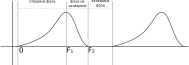
\includegraphics[width=0.9\textwidth]{glotal_pulse}%
        }
        \pause
        \begin{columns}[c]
            \begin{column}{0.65\textwidth}
                \begin{flalign*}
                    & g(t) = 
                    \begin{cases}
                        \cfrac{1}{2}( 1 - \cos{(\pi n / F1)}), & 0\leq t \leq F_1\\
                        \cos{(\pi(n - F_1)/2(F_2 - F_1))}, & F_1 \leq t \leq F_2\\
                        0, & \text{иначе}   
                    \end{cases}   &&     
                \end{flalign*}
            \end{column}
            \pause
            \begin{column}{0.35\textwidth}
                \begin{align*}
                    \mathcal{G}(z) = \frac{1}{(1 - \beta z)^2}
                \end{align*}
            \end{column}
        \end{columns}
    \end{frame}

    \begin{frame}[t]{Сигнал от реч - модел на тръбите}
        \begin{columns}[c]
            \begin{column}{0.48\textwidth}
                {\tiny \begin{flalign*}
                    & \mathcal{V}(z) = \frac{0.5(1+r_G)\prod\limits_{i=1}^{N}{(1 + r_i)} z^{-N/2}}{1 - \sum\limits_{i=1}^{N}{\alpha_i z^{-i}}} &&
                \end{flalign*}}
            \end{column}%
            \hfill%
            \begin{column}{0.14\textwidth}
                {\tiny \begin{flalign*}
                    & \mathcal{R}(z) = 1 - \gamma z^{-1} &&
                \end{flalign*}}
            \end{column}%
            \hfill%
            \begin{column}{0.34\textwidth}
            \end{column}%
        \end{columns}
        \centering{Общ вид на $\mathcal{G}$}
        
        \centering{
            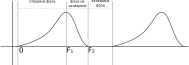
\includegraphics[width=0.9\textwidth]{glotal_pulse}%
        }
        \begin{columns}[c]
            \begin{column}{0.65\textwidth}
                \begin{flalign*}
                    & g(t) = 
                    \begin{cases}
                        \cfrac{1}{2}( 1 - \cos{(\pi n / F1)}), & 0\leq t \leq F_1\\
                        \cos{(\pi(n - F_1)/2(F_2 - F_1))}, & F_1 \leq t \leq F_2\\
                        0, & \text{иначе}   
                    \end{cases}   &&     
                \end{flalign*}
            \end{column}
            \begin{column}{0.35\textwidth}
                \begin{align*}
                    \mathcal{G}(z) = \frac{\prod\limits_{i=0}^K (1 - \beta_i z^{-1})}{(1 - \beta z)^2}
                \end{align*}
            \end{column}
        \end{columns}
    \end{frame}

    \begin{frame}[t]{Сигнал от реч - модел на тръбите}
        \begin{columns}[c]
            \begin{column}{0.48\textwidth}
                {\tiny \begin{flalign*}
                    & \mathcal{V}(z) = \frac{0.5(1+r_G)\prod\limits_{i=1}^{N}{(1 + r_i)} z^{-N/2}}{1 - \sum\limits_{i=1}^{N}{\alpha_i z^{-i}}} &&
                \end{flalign*}}
            \end{column}%
            \hfill%
            \begin{column}{0.14\textwidth}
                {\tiny \begin{flalign*}
                    & \mathcal{R}(z) = 1 - \gamma z^{-1} &&
                \end{flalign*}}
            \end{column}%
            \hfill%
            \begin{column}{0.34\textwidth}
                {\tiny \begin{align*}
                    \mathcal{G}(z) = \frac{\prod\limits_{i=0}^K (1 - \beta_i z^{-1})}{(1 - \beta z)^2}
                \end{align*}}
            \end{column}%
        \end{columns}
        \centering{Общ вид на $\mathcal{G}$}
        
        \centering{
            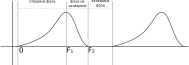
\includegraphics[width=0.9\textwidth]{glotal_pulse}%
        }
        \begin{columns}[c]
            \begin{column}{0.65\textwidth}
                \begin{flalign*}
                    & g(t) = 
                    \begin{cases}
                        \cfrac{1}{2}( 1 - \cos{(\pi n / F1)}), & 0\leq t \leq F_1\\
                        \cos{(\pi(n - F_1)/2(F_2 - F_1))}, & F_1 \leq t \leq F_2\\
                        0, & \text{иначе}   
                    \end{cases}   &&     
                \end{flalign*}
            \end{column}
            \begin{column}{0.35\textwidth}
                \begin{align*}
                    \mathcal{G}(z) = \frac{\prod\limits_{i=0}^K (1 - \beta_i z^{-1})}{(1 - \beta z)^2}
                \end{align*}
            \end{column}
        \end{columns}
    \end{frame}

    \begin{frame}[t]{Сигнал от реч - модел на тръбите}
        \begin{columns}[c]
            \begin{column}{0.48\textwidth}
                {\tiny \begin{flalign*}
                    & \mathcal{V}(z) = \frac{0.5(1+r_G)\prod\limits_{i=1}^{N}{(1 + r_i)} z^{-N/2}}{1 - \sum\limits_{i=1}^{N}{\alpha_i z^{-i}}} &&
                \end{flalign*}}
            \end{column}%
            \hfill%
            \begin{column}{0.14\textwidth}
                {\tiny \begin{flalign*}
                    & \mathcal{R}(z) = 1 - \gamma z^{-1} &&
                \end{flalign*}}
            \end{column}%
            \hfill%
            \begin{column}{0.34\textwidth}
                {\tiny \begin{align*}
                    \mathcal{G}(z) = \frac{\prod\limits_{i=0}^K (1 - \beta_i z^{-1})}{(1 - \beta z)^2}
                \end{align*}}
            \end{column}%
        \end{columns}
        \pause
        \centering{Общ вид на $\mathcal{Y}$}
        \pause
        \begin{flalign*}
            & \mathcal{Y}(z) = \mathcal{G}(z) \mathcal{V}(z) \mathcal{R}(z) &&
        \end{flalign*}
        \pause

        \begin{flalign*}
            & = \Q{\frac{\prod\limits_{i=0}^K (1 - \beta_i z^{-1})}{(1 - \beta z)^2}} \Q{\frac{0.5(1+r_G)\prod\limits_{i=1}^{N}{(1 + r_i)} z^{-N/2}}{1 - \sum\limits_{i=1}^{N}{\alpha_i z^{-i}}}} \Q{\frac{\prod\limits_{i=0}^K (1 - \beta_i z^{-1})}{(1 - \beta z)^2}} &&
        \end{flalign*}
    
        \pause
        \begin{flalign*}
            & = \mathcal{G}(z) \cfrac{\sum\limits_{m=0}^{M} b_m z^{-m} }{\sum\limits_{k=0}^{K} a_k z^{-k}}, &&
        \end{flalign*}
    \end{frame}

    \begin{frame}[t]{Сигнал от реч - модел на тръбите}
        \begin{columns}[c]
            \hfill            
            \begin{column}{0.38\textwidth}
                {\tiny 
                \begin{flalign*}
                    & \mathcal{Y}(z) = \mathcal{G}(z)\mathcal{V}(z)\mathcal{R}(z) = \mathcal{G}(z) \cfrac{\sum\limits_{m=0}^{M} b_m z^{-m} }{\sum\limits_{k=0}^{K} a_k z^{-k}} &&
                \end{flalign*}}
            \end{column}
            \hfill
        \end{columns}
        \centering{Общ вид на $\mathcal{Y}$}
        \begin{flalign*}
            & \mathcal{Y}(z) = \mathcal{G}(z) \mathcal{V}(z) \mathcal{R}(z) &&
        \end{flalign*}

        \begin{flalign*}
            & = \Q{\frac{\prod\limits_{i=0}^K (1 - \beta_i z^{-1})}{(1 - \beta z)^2}} \Q{\frac{0.5(1+r_G)\prod\limits_{i=1}^{N}{(1 + r_i)} z^{-N/2}}{1 - \sum\limits_{i=1}^{N}{\alpha_i z^{-i}}}} \Q{\frac{\prod\limits_{i=0}^K (1 - \beta_i z^{-1})}{(1 - \beta z)^2}} &&
        \end{flalign*}
    
        \begin{flalign*}
            & = \mathcal{G}(z) \cfrac{\sum\limits_{m=0}^{M} b_m z^{-m} }{\sum\limits_{k=0}^{K} a_k z^{-k}}, &&
        \end{flalign*}
    \end{frame}

    \begin{frame}[t]{Сигнал от реч - представяне със системи}
        \begin{columns}[c]
            \hfill            
            \begin{column}{0.38\textwidth}
                {\tiny 
                \begin{flalign*}
                    & \mathcal{Y}(z) = \mathcal{G}(z)\mathcal{V}(z)\mathcal{R}(z) = \mathcal{G}(z) \cfrac{\sum\limits_{m=0}^{M} b_m z^{-m} }{\sum\limits_{k=0}^{K} a_k z^{-k}} &&
                \end{flalign*}}
            \end{column}
            \hfill
        \end{columns}
            \pause
            \begin{itemize}
                \item Система (дефиниция)
                \pause
                 - Механизъм, който манипулира един или повече сигнали с някаква цел до получаване на нов сигнал, се нарича система.
                \pause
                \item Филтър
                \pause
                \item $g[n] \mapsto y[n]$
                \pause
                \item Линейна система (Дефиниция)
                \pause
                 - Ако $x_1[n] \mapsto y_1[n]$ и $x_2[n] \mapsto y_2[n]$, то системата е линейна $\longleftrightarrow$

                $\forall a, b \in \mathbb{R} \B{ax_1[n] + bx_2[n] \mapsto ay_1[n] + by_2[n]}$ 
                \pause
                \item Времево-инвариантна система (Дефиниция)
                \pause
                - Нека $x[n] \mapsto y[n]$. Тогава, ако за всяко $n_0: x[n - n_0] \mapsto y[n - n_0]$, то
                системата е времево-инвариантна.
                \pause
                \item $\sum\limits_{k=0}^{N} a_k y [n-k] = \sum\limits_{m=0}^{M}b_m x[n-m] $
            \end{itemize}
    \end{frame}

    \begin{frame}[t]{Сигнал от реч - представяне със системи}
        \begin{columns}[c]
            \hfill            
            \begin{column}{0.38\textwidth}
                {\tiny 
                \begin{flalign*}
                    & \mathcal{Y}(z) = \mathcal{G}(z)\mathcal{V}(z)\mathcal{R}(z) = \mathcal{G}(z) \cfrac{\sum\limits_{m=0}^{M} b_m z^{-m} }{\sum\limits_{k=0}^{K} a_k z^{-k}} &&
                \end{flalign*}}
            \end{column}
            \begin{column}{0.38\textwidth}
                {\tiny $\sum\limits_{k=0}^{N} a_k y [n-k] = \sum\limits_{m=0}^{M}b_m x[n-m] $}
            \end{column}
        \end{columns}
            \begin{itemize}
                \item Система (дефиниция)
                 - Механизъм, който манипулира един или повече сигнали с някаква цел до получаване на нов сигнал, се нарича система.
                \item Филтър
                \item $g[n] \mapsto y[n]$
                \item Линейна система (Дефиниция)
                 - Ако $x_1[n] \mapsto y_1[n]$ и $x_2[n] \mapsto y_2[n]$, то системата е линейна $\longleftrightarrow$

                $\forall a, b \in \mathbb{R} \B{ax_1[n] + bx_2[n] \mapsto ay_1[n] + by_2[n]}$ 
                \item Времево-инвариантна система (Дефиниция)
                - Нека $x[n] \mapsto y[n]$. Тогава, ако за всяко $n_0: x[n - n_0] \mapsto y[n - n_0]$, то
                системата е времево-инвариантна.
                \item $\sum\limits_{k=0}^{N} a_k y [n-k] = \sum\limits_{m=0}^{M}b_m x[n-m] $
            \end{itemize}
    \end{frame}

    \begin{frame}[t]{Сигнал от реч - представяне със системи}
        \begin{columns}[c]
            \hfill            
            \begin{column}{0.38\textwidth}
                {\tiny 
                \begin{flalign*}
                    & \mathcal{Y}(z) = \mathcal{G}(z)\mathcal{V}(z)\mathcal{R}(z) = \mathcal{G}(z) \cfrac{\sum\limits_{m=0}^{M} b_m z^{-m} }{\sum\limits_{k=0}^{K} a_k z^{-k}} &&
                \end{flalign*}}
            \end{column}
            \begin{column}{0.38\textwidth}
                {\tiny $\sum\limits_{k=0}^{N} a_k y [n-k] = \sum\limits_{m=0}^{M}b_m x[n-m] $}
            \end{column}
        \end{columns}
        \pause
        Нека имаме линейна времево-инвариантна система.
    \end{frame}

    \begin{frame}[t]{Сигнал от реч - представяне със системи}
        \begin{columns}[c]
            \hfill            
            \begin{column}{0.38\textwidth}
                {\tiny 
                \begin{flalign*}
                    & \mathcal{Y}(z) = \mathcal{G}(z)\mathcal{V}(z)\mathcal{R}(z) = \mathcal{G}(z) \cfrac{\sum\limits_{m=0}^{M} b_m z^{-m} }{\sum\limits_{k=0}^{K} a_k z^{-k}} &&
                \end{flalign*}}
            \end{column}
            \begin{column}{0.38\textwidth}
                {\tiny $\sum\limits_{k=0}^{N} a_k y [n-k] = \sum\limits_{m=0}^{M}b_m x[n-m] $}
            \end{column}
        \end{columns}
        Нека имаме линейна времево-инвариантна система.
        \begin{columns}[T]
            \begin{column}{0.68\textwidth}
                \begin{flalign*}
                    & g[n] &&
                \end{flalign*}
            \end{column}
            \hfill
            \begin{column}{0.28\textwidth}
            \end{column}
        \end{columns}
    \end{frame}

    \begin{frame}[t]{Сигнал от реч - представяне със системи}
        \begin{columns}[c]
            \hfill            
            \begin{column}{0.38\textwidth}
                {\tiny 
                \begin{flalign*}
                    & \mathcal{Y}(z) = \mathcal{G}(z)\mathcal{V}(z)\mathcal{R}(z) = \mathcal{G}(z) \cfrac{\sum\limits_{m=0}^{M} b_m z^{-m} }{\sum\limits_{k=0}^{K} a_k z^{-k}} &&
                \end{flalign*}}
            \end{column}
            \begin{column}{0.38\textwidth}
                {\tiny $\sum\limits_{k=0}^{N} a_k y [n-k] = \sum\limits_{m=0}^{M}b_m x[n-m] $}
            \end{column}
        \end{columns}
        Нека имаме линейна времево-инвариантна система.
        \begin{columns}[T]
            \begin{column}{0.68\textwidth}
                \begin{flalign*}
                    & g[n] &&
                \end{flalign*}
            \end{column}
            \hfill
            \begin{column}{0.28\textwidth}
                \begin{flalign*}
                    &\delta[n] = \begin{cases}
                        1, & n = 0\\
                        0, & \text{иначе}\\
                        \end{cases} && 
                \end{flalign*}
            \end{column}
        \end{columns}
    \end{frame}

    \begin{frame}[t]{Сигнал от реч - представяне със системи}
        \begin{columns}[c]
            \hfill            
            \begin{column}{0.38\textwidth}
                {\tiny 
                \begin{flalign*}
                    & \mathcal{Y}(z) = \mathcal{G}(z)\mathcal{V}(z)\mathcal{R}(z) = \mathcal{G}(z) \cfrac{\sum\limits_{m=0}^{M} b_m z^{-m} }{\sum\limits_{k=0}^{K} a_k z^{-k}} &&
                \end{flalign*}}
            \end{column}
            \begin{column}{0.38\textwidth}
                {\tiny $\sum\limits_{k=0}^{N} a_k y [n-k] = \sum\limits_{m=0}^{M}b_m x[n-m] $}
            \end{column}
        \end{columns}
        Нека имаме линейна времево-инвариантна система.
        \begin{columns}[T]
            \begin{column}{0.68\textwidth}
                \begin{flalign*}
                    & g[n] = \sum\limits_{k=-\infty}^{\infty} g[k]\delta[n-k] &&
                \end{flalign*}
            \end{column}
            \hfill
            \begin{column}{0.28\textwidth}
                \begin{flalign*}
                    &\delta[n] = \begin{cases}
                        1, & n = 0\\
                        0, & \text{иначе}\\
                        \end{cases} && 
                \end{flalign*}
            \end{column}
        \end{columns}
    \end{frame}

    \begin{frame}[t]{Сигнал от реч - представяне със системи}
        \begin{columns}[c]
            \hfill            
            \begin{column}{0.38\textwidth}
                {\tiny 
                \begin{flalign*}
                    & \mathcal{Y}(z) = \mathcal{G}(z)\mathcal{V}(z)\mathcal{R}(z) = \mathcal{G}(z) \cfrac{\sum\limits_{m=0}^{M} b_m z^{-m} }{\sum\limits_{k=0}^{K} a_k z^{-k}} &&
                \end{flalign*}}
            \end{column}
            \begin{column}{0.38\textwidth}
                {\tiny $\sum\limits_{k=0}^{N} a_k y [n-k] = \sum\limits_{m=0}^{M}b_m x[n-m] $}
            \end{column}
        \end{columns}
        Нека имаме линейна времево-инвариантна система.
        \begin{columns}[T]
            \begin{column}{0.68\textwidth}
                \begin{flalign*}
                    & g[n] = \sum\limits_{k=-\infty}^{\infty} g[k]\delta[n-k] &&
                \end{flalign*}
                Ако $\delta[n-k] \mapsto h_k[n]$, тъй като системата е линейна:
            \end{column}
            \hfill
            \begin{column}{0.28\textwidth}
                \begin{flalign*}
                    &\delta[n] = \begin{cases}
                        1, & n = 0\\
                        0, & \text{иначе}\\
                        \end{cases} && 
                \end{flalign*}
            \end{column}
        \end{columns}
    \end{frame}

    \begin{frame}[t]{Сигнал от реч - представяне със системи}
        \begin{columns}[c]
            \hfill            
            \begin{column}{0.38\textwidth}
                {\tiny 
                \begin{flalign*}
                    & \mathcal{Y}(z) = \mathcal{G}(z)\mathcal{V}(z)\mathcal{R}(z) = \mathcal{G}(z) \cfrac{\sum\limits_{m=0}^{M} b_m z^{-m} }{\sum\limits_{k=0}^{K} a_k z^{-k}} &&
                \end{flalign*}}
            \end{column}
            \begin{column}{0.38\textwidth}
                {\tiny $\sum\limits_{k=0}^{N} a_k y [n-k] = \sum\limits_{m=0}^{M}b_m x[n-m] $}
            \end{column}
        \end{columns}
        Нека имаме линейна времево-инвариантна система.
        \begin{columns}[T]
            \begin{column}{0.68\textwidth}
                \begin{flalign*}
                    & g[n] = \sum\limits_{k=-\infty}^{\infty} g[k]\delta[n-k] &&
                \end{flalign*}
                Ако $\delta[n-k] \mapsto h_k[n]$, тъй като системата е линейна:
                \begin{flalign*}
                    & g[n] = \sum\limits_{k=-\infty}^{\infty}g[k]\delta[n-k] \mapsto \sum\limits_{k = -\infty}^{\infty}g[k]h_k[n] = y[n] &&
                \end{flalign*}
            \end{column}
            \hfill
            \begin{column}{0.28\textwidth}
                \begin{flalign*}
                    &\delta[n] = \begin{cases}
                        1, & n = 0\\
                        0, & \text{иначе}\\
                        \end{cases} && 
                \end{flalign*}
            \end{column}
        \end{columns}
    \end{frame}

    \begin{frame}[t]{Сигнал от реч - представяне със системи}
        \begin{columns}[c]
            \hfill            
            \begin{column}{0.38\textwidth}
                {\tiny 
                \begin{flalign*}
                    & \mathcal{Y}(z) = \mathcal{G}(z)\mathcal{V}(z)\mathcal{R}(z) = \mathcal{G}(z) \cfrac{\sum\limits_{m=0}^{M} b_m z^{-m} }{\sum\limits_{k=0}^{K} a_k z^{-k}} &&
                \end{flalign*}}
            \end{column}
            \begin{column}{0.38\textwidth}
                {\tiny $\sum\limits_{k=0}^{N} a_k y [n-k] = \sum\limits_{m=0}^{M}b_m x[n-m] $}
            \end{column}
        \end{columns}
        Нека имаме линейна времево-инвариантна система.
        \begin{columns}[T]
            \begin{column}{0.68\textwidth}
                \begin{flalign*}
                    & g[n] = \sum\limits_{k=-\infty}^{\infty} g[k]\delta[n-k] &&
                \end{flalign*}
                Ако $\delta[n-k] \mapsto h_k[n]$, тъй като системата е линейна:
                \begin{flalign*}
                    & g[n] = \sum\limits_{k=-\infty}^{\infty}g[k]\delta[n-k] \mapsto \sum\limits_{k = -\infty}^{\infty}g[k]h_k[n] = y[n] &&
                \end{flalign*}
            \end{column}
            \hfill
            \begin{column}{0.28\textwidth}
                \begin{flalign*}
                    &\delta[n] = \begin{cases}
                        1, & n = 0\\
                        0, & \text{иначе}\\
                    \end{cases} && 
                \end{flalign*}
            \end{column}
        \end{columns}
        От времевата инвариантност, ако  $\delta[n] \mapsto h[n]$, то $\delta[n -k] \mapsto h[n-k]$, следователно:
    \end{frame}

    \begin{frame}[t]{Сигнал от реч - представяне със системи}
        \begin{columns}[c]
            \hfill            
            \begin{column}{0.38\textwidth}
                {\tiny 
                \begin{flalign*}
                    & \mathcal{Y}(z) = \mathcal{G}(z)\mathcal{V}(z)\mathcal{R}(z) = \mathcal{G}(z) \cfrac{\sum\limits_{m=0}^{M} b_m z^{-m} }{\sum\limits_{k=0}^{K} a_k z^{-k}} &&
                \end{flalign*}}
            \end{column}
            \begin{column}{0.38\textwidth}
                {\tiny $\sum\limits_{k=0}^{N} a_k y [n-k] = \sum\limits_{m=0}^{M}b_m x[n-m] $}
            \end{column}
        \end{columns}
        Нека имаме линейна времево-инвариантна система.
        \begin{columns}[T]
            \begin{column}{0.68\textwidth}
                \begin{flalign*}
                    & g[n] = \sum\limits_{k=-\infty}^{\infty} g[k]\delta[n-k] &&
                \end{flalign*}
                Ако $\delta[n-k] \mapsto h_k[n]$, тъй като системата е линейна:
                \begin{flalign*}
                    & g[n] = \sum\limits_{k=-\infty}^{\infty}g[k]\delta[n-k] \mapsto \sum\limits_{k = -\infty}^{\infty}g[k]h_k[n] = y[n] &&
                \end{flalign*}
            \end{column}
            \hfill
            \begin{column}{0.28\textwidth}
                \begin{flalign*}
                    &\delta[n] = \begin{cases}
                        1, & n = 0\\
                        0, & \text{иначе}\\
                    \end{cases} && 
                \end{flalign*}
            \end{column}
        \end{columns}
        От времевата инвариантност, ако  $\delta[n] \mapsto h[n]$, то $\delta[n -k] \mapsto h[n-k]$, следователно:
        \begin{flalign*}
            &  y[n] = \sum\limits_{k = -\infty}^{\infty}g[k]h_k[n] = \sum\limits_{k = -\infty}^{\infty}g[k]h[n-k] &&
        \end{flalign*}
    \end{frame}

    \begin{frame}[t]{Сигнал от реч - представяне със системи}
        \begin{columns}[c]
            \hfill            
            \begin{column}{0.38\textwidth}
                {\tiny 
                \begin{flalign*}
                    & \mathcal{Y}(z) = \mathcal{G}(z)\mathcal{V}(z)\mathcal{R}(z) = \mathcal{G}(z) \cfrac{\sum\limits_{m=0}^{M} b_m z^{-m} }{\sum\limits_{k=0}^{K} a_k z^{-k}} &&
                \end{flalign*}}
            \end{column}
            \begin{column}{0.38\textwidth}
                {\tiny $\sum\limits_{k=0}^{N} a_k y [n-k] = \sum\limits_{m=0}^{M}b_m x[n-m] $}
            \end{column}
        \end{columns}
        Нека имаме линейна времево-инвариантна система.
        \begin{columns}[T]
            \begin{column}{0.68\textwidth}
                \begin{flalign*}
                    & g[n] = \sum\limits_{k=-\infty}^{\infty} g[k]\delta[n-k] &&
                \end{flalign*}
                Ако $\delta[n-k] \mapsto h_k[n]$, тъй като системата е линейна:
                \begin{flalign*}
                    & g[n] = \sum\limits_{k=-\infty}^{\infty}g[k]\delta[n-k] \mapsto \sum\limits_{k = -\infty}^{\infty}g[k]h_k[n] = y[n] &&
                \end{flalign*}
            \end{column}
            \hfill
            \begin{column}{0.28\textwidth}
                \begin{flalign*}
                    &\delta[n] = \begin{cases}
                        1, & n = 0\\
                        0, & \text{иначе}\\
                    \end{cases} && 
                \end{flalign*}
            \end{column}
        \end{columns}
        От времевата инвариантност, ако  $\delta[n] \mapsto h[n]$, то $\delta[n -k] \mapsto h[n-k]$, следователно:
        \begin{flalign*}
            &  y[n] = \sum\limits_{k = -\infty}^{\infty}g[k]h_k[n] = \sum\limits_{k = -\infty}^{\infty}g[k]h[n-k] = (g\ast h)[n]&&
        \end{flalign*}
    \end{frame}

    \begin{frame}[t]{Сигнал от реч - представяне със системи}
        \begin{columns}[c]
            \hfill            
            \begin{column}{0.38\textwidth}
                {\tiny 
                \begin{flalign*}
                    & \mathcal{Y}(z) = \mathcal{G}(z)\mathcal{V}(z)\mathcal{R}(z) = \mathcal{G}(z) \cfrac{\sum\limits_{m=0}^{M} b_m z^{-m} }{\sum\limits_{k=0}^{K} a_k z^{-k}} &&
                \end{flalign*}}
            \end{column}
            \begin{column}{0.38\textwidth}
                {\tiny $\sum\limits_{k=0}^{N} a_k y [n-k] = \sum\limits_{m=0}^{M}b_m x[n-m] $}
            \end{column}
        \end{columns}
        \begin{flalign*}
            &  y[n] = (g\ast h)[n]&&
        \end{flalign*}
    \end{frame}

    \begin{frame}[t]{Сигнал от реч - представяне със системи}
        \begin{columns}[c]
            \hfill            
            \begin{column}{0.38\textwidth}
                {\tiny 
                \begin{flalign*}
                    & \mathcal{Y}(z) = \mathcal{G}(z)\mathcal{V}(z)\mathcal{R}(z) = \mathcal{G}(z) \cfrac{\sum\limits_{m=0}^{M} b_m z^{-m} }{\sum\limits_{k=0}^{K} a_k z^{-k}} &&
                \end{flalign*}}
            \end{column}
            \begin{column}{0.38\textwidth}
                {\tiny $\sum\limits_{k=0}^{N} a_k y [n-k] = \sum\limits_{m=0}^{M}b_m x[n-m] $}
            \end{column}
        \end{columns}
        \begin{flalign*}
            &  y[n] = (g\ast h)[n]\qquad \qquad y[n] \xleftrightarrow{\mathcal{F}\mathcal{S}} Y(z), g[n]\xleftrightarrow{\mathcal{F}\mathcal{S}} G(z), h[n] \xleftrightarrow{\mathcal{F}\mathcal{S}} H(z), z = e^{iw}&&
        \end{flalign*}
    \end{frame}

    \begin{frame}[t]{Сигнал от реч - представяне със системи}
        \begin{columns}[c]
            \hfill            
            \begin{column}{0.38\textwidth}
                {\tiny 
                \begin{flalign*}
                    & \mathcal{Y}(z) = \mathcal{G}(z)\mathcal{V}(z)\mathcal{R}(z) = \mathcal{G}(z) \cfrac{\sum\limits_{m=0}^{M} b_m z^{-m} }{\sum\limits_{k=0}^{K} a_k z^{-k}} &&
                \end{flalign*}}
            \end{column}
            \begin{column}{0.38\textwidth}
                {\tiny $\sum\limits_{k=0}^{N} a_k y [n-k] = \sum\limits_{m=0}^{M}b_m x[n-m] $}
            \end{column}
        \end{columns}
        \begin{flalign*}
            &  y[n] = (g\ast h)[n]\qquad \qquad y[n] \xleftrightarrow{\mathcal{F}\mathcal{S}} Y(z), g[n]\xleftrightarrow{\mathcal{F}\mathcal{S}} G(z), h[n] \xleftrightarrow{\mathcal{F}\mathcal{S}} H(z), z = e^{iw}&&\\
            &Y(z) = G(z)H(z) &&
        \end{flalign*}
    \end{frame}

    \begin{frame}[t]{Сигнал от реч - представяне със системи}
        \begin{columns}[c]
            \hfill            
            \begin{column}{0.38\textwidth}
                {\tiny 
                \begin{flalign*}
                    & \mathcal{Y}(z) = \mathcal{G}(z)\mathcal{V}(z)\mathcal{R}(z) = \mathcal{G}(z) \cfrac{\sum\limits_{m=0}^{M} b_m z^{-m} }{\sum\limits_{k=0}^{K} a_k z^{-k}} &&
                \end{flalign*}}
            \end{column}
            \begin{column}{0.38\textwidth}
                {\tiny $\sum\limits_{k=0}^{N} a_k y [n-k] = \sum\limits_{m=0}^{M}b_m x[n-m] $}
            \end{column}
        \end{columns}
        \begin{flalign*}
            &  y[n] = (g\ast h)[n]\qquad \qquad y[n] \xleftrightarrow{\mathcal{F}\mathcal{S}} Y(z), g[n]\xleftrightarrow{\mathcal{F}\mathcal{S}} G(z), h[n] \xleftrightarrow{\mathcal{F}\mathcal{S}} H(z), z = e^{iw}&&\\
            &Y(z) = G(z)H(z) &&\\
            & H(z) = \cfrac{Y(z)}{G(z)} &&
        \end{flalign*}
    \end{frame}

    \begin{frame}[t]{Сигнал от реч - представяне със системи}
        \begin{columns}[c]
            \hfill            
            \begin{column}{0.38\textwidth}
                {\tiny 
                \begin{flalign*}
                    & \mathcal{Y}(z) = \mathcal{G}(z)\mathcal{V}(z)\mathcal{R}(z) = \mathcal{G}(z) \cfrac{\sum\limits_{m=0}^{M} b_m z^{-m} }{\sum\limits_{k=0}^{K} a_k z^{-k}} &&
                \end{flalign*}}
            \end{column}
            \begin{column}{0.38\textwidth}
                {\tiny $\sum\limits_{k=0}^{N} a_k y [n-k] = \sum\limits_{m=0}^{M}b_m x[n-m] $}
            \end{column}
        \end{columns}
        \begin{flalign*}
            &  y[n] = (g\ast h)[n]\qquad \qquad y[n] \xleftrightarrow{\mathcal{F}\mathcal{S}} Y(z), g[n]\xleftrightarrow{\mathcal{F}\mathcal{S}} G(z), h[n] \xleftrightarrow{\mathcal{F}\mathcal{S}} H(z), z = e^{iw}&&\\
            &Y(z) = G(z)H(z) &&\\
            & H(z) = \cfrac{Y(z)}{G(z)} \text{ - предавателна функция} &&
        \end{flalign*}
    \end{frame}

    \begin{frame}[t]{Сигнал от реч - представяне със системи}
        \begin{columns}[c]
            \hfill            
            \begin{column}{0.38\textwidth}
                {\tiny 
                \begin{flalign*}
                    & \mathcal{Y}(z) = \mathcal{G}(z)\mathcal{V}(z)\mathcal{R}(z) = \mathcal{G}(z) \cfrac{\sum\limits_{m=0}^{M} b_m z^{-m} }{\sum\limits_{k=0}^{K} a_k z^{-k}} &&
                \end{flalign*}}
            \end{column}
            \begin{column}{0.38\textwidth}
                {\color{mypink} {\tiny $\sum\limits_{k=0}^{N} a_k y [n-k] = \sum\limits_{m=0}^{M}b_m x[n-m] $}}
            \end{column}
        \end{columns}
        \begin{flalign*}
            &  y[n] = (g\ast h)[n]\qquad \qquad y[n] \xleftrightarrow{\mathcal{F}\mathcal{S}} Y(z), g[n]\xleftrightarrow{\mathcal{F}\mathcal{S}} G(z), h[n] \xleftrightarrow{\mathcal{F}\mathcal{S}} H(z), z = e^{iw}&&\\
            &Y(z) = G(z)H(z) &&\\
            & H(z) = \cfrac{Y(z)}{G(z)} \text{ - предавателна функция} &&
        \end{flalign*}
    \end{frame}

    \begin{frame}[t]{Сигнал от реч - представяне със системи}
        \begin{columns}[c]
            \hfill            
            \begin{column}{0.38\textwidth}
                {\tiny 
                \begin{flalign*}
                    & \mathcal{Y}(z) = \mathcal{G}(z)\mathcal{V}(z)\mathcal{R}(z) = \mathcal{G}(z) \cfrac{\sum\limits_{m=0}^{M} b_m z^{-m} }{\sum\limits_{k=0}^{K} a_k z^{-k}} &&
                \end{flalign*}}
            \end{column}
            \begin{column}{0.38\textwidth}
                {\color{mypink} {\tiny $\sum\limits_{k=0}^{N} a_k y [n-k] = \sum\limits_{m=0}^{M}b_m x[n-m] $}}
            \end{column}
        \end{columns}
        \begin{flalign*}
            &  y[n] = (g\ast h)[n]\qquad \qquad y[n] \xleftrightarrow{\mathcal{F}\mathcal{S}} Y(z), g[n]\xleftrightarrow{\mathcal{F}\mathcal{S}} G(z), h[n] \xleftrightarrow{\mathcal{F}\mathcal{S}} H(z), z = e^{iw}&&\\
            &Y(z) = G(z)H(z) &&\\
            & H(z) = \cfrac{Y(z)}{G(z)} \text{ - предавателна функция} && \\
            & \sum\limits_{k=0}^{N} a_k y [n-k] = \sum\limits_{m=0}^{M}b_m g[n-m] &&
        \end{flalign*}
    \end{frame}

    \begin{frame}[t]{Сигнал от реч - представяне със системи}
        \begin{columns}[c]
            \hfill            
            \begin{column}{0.38\textwidth}
                {\tiny 
                \begin{flalign*}
                    & \mathcal{Y}(z) = \mathcal{G}(z)\mathcal{V}(z)\mathcal{R}(z) = \mathcal{G}(z) \cfrac{\sum\limits_{m=0}^{M} b_m z^{-m} }{\sum\limits_{k=0}^{K} a_k z^{-k}} &&
                \end{flalign*}}
            \end{column}
            \begin{column}{0.38\textwidth}
                {\tiny $\sum\limits_{k=0}^{N} a_k y [n-k] = \sum\limits_{m=0}^{M}b_m x[n-m] $}
            \end{column}
        \end{columns}
        \begin{flalign*}
            &  y[n] = (g\ast h)[n]\qquad \qquad y[n] \xleftrightarrow{\mathcal{F}\mathcal{S}} Y(z), g[n]\xleftrightarrow{\mathcal{F}\mathcal{S}} G(z), h[n] \xleftrightarrow{\mathcal{F}\mathcal{S}} H(z), z = e^{iw}&&\\
            &Y(z) = G(z)H(z) &&\\
            & H(z) = \cfrac{Y(z)}{G(z)} \text{ - предавателна функция} && \\
            & \sum\limits_{k=0}^{N} a_k y [n-k] = \sum\limits_{m=0}^{M}b_m g[n-m] \qquad \qquad y[n] \xleftrightarrow{\mathcal{F}\mathcal{S}} Y(z), g[n]\xleftrightarrow{\mathcal{F}\mathcal{S}} G(z)&&
        \end{flalign*}
    \end{frame}

    \begin{frame}[t]{Сигнал от реч - представяне със системи}
        \begin{columns}[c]
            \hfill            
            \begin{column}{0.38\textwidth}
                {\tiny 
                \begin{flalign*}
                    & \mathcal{Y}(z) = \mathcal{G}(z)\mathcal{V}(z)\mathcal{R}(z) = \mathcal{G}(z) \cfrac{\sum\limits_{m=0}^{M} b_m z^{-m} }{\sum\limits_{k=0}^{K} a_k z^{-k}} &&
                \end{flalign*}}
            \end{column}
            \begin{column}{0.38\textwidth}
                {\tiny $\sum\limits_{k=0}^{N} a_k y [n-k] = \sum\limits_{m=0}^{M}b_m x[n-m] $}
            \end{column}
        \end{columns}
        \begin{flalign*}
            &  y[n] = (g\ast h)[n]\qquad \qquad y[n] \xleftrightarrow{\mathcal{F}\mathcal{S}} Y(z), g[n]\xleftrightarrow{\mathcal{F}\mathcal{S}} G(z), h[n] \xleftrightarrow{\mathcal{F}\mathcal{S}} H(z), z = e^{iw}&&\\
            &Y(z) = G(z)H(z) &&\\
            & H(z) = \cfrac{Y(z)}{G(z)} \text{ - предавателна функция} && \\
            & \sum\limits_{k=0}^{N} a_k y [n-k] = \sum\limits_{m=0}^{M}b_m g[n-m] \qquad \qquad y[n] \xleftrightarrow{\mathcal{F}\mathcal{S}} Y(z), g[n]\xleftrightarrow{\mathcal{F}\mathcal{S}} G(z)&&\\
            & \nonumber\Q{\sum\limits_{k=0}^{N}a_k z^{-k}}\mathcal{Y}( z) = \Q{\sum\limits_{m=0}^{M} b_m  z^{-m}}\mathcal{G}( z) &&
        \end{flalign*}
    \end{frame}

    \begin{frame}[t]{Сигнал от реч - представяне със системи}
        \begin{columns}[c]
            \hfill            
            \begin{column}{0.38\textwidth}
                {\tiny 
                \begin{flalign*}
                    & \mathcal{Y}(z) = \mathcal{G}(z)\mathcal{V}(z)\mathcal{R}(z) = \mathcal{G}(z) \cfrac{\sum\limits_{m=0}^{M} b_m z^{-m} }{\sum\limits_{k=0}^{K} a_k z^{-k}} &&
                \end{flalign*}}
            \end{column}
            \begin{column}{0.38\textwidth}
                {\tiny $\sum\limits_{k=0}^{N} a_k y [n-k] = \sum\limits_{m=0}^{M}b_m x[n-m] $}
            \end{column}
        \end{columns}
        \begin{flalign*}
            &  y[n] = (g\ast h)[n]\qquad \qquad y[n] \xleftrightarrow{\mathcal{F}\mathcal{S}} Y(z), g[n]\xleftrightarrow{\mathcal{F}\mathcal{S}} G(z), h[n] \xleftrightarrow{\mathcal{F}\mathcal{S}} H(z), z = e^{iw}&&\\
            &Y(z) = G(z)H(z) &&\\
            & H(z) = \cfrac{Y(z)}{G(z)} \text{ - предавателна функция} && \\
            & \sum\limits_{k=0}^{N} a_k y [n-k] = \sum\limits_{m=0}^{M}b_m g[n-m] \qquad \qquad y[n] \xleftrightarrow{\mathcal{F}\mathcal{S}} Y(z), g[n]\xleftrightarrow{\mathcal{F}\mathcal{S}} G(z)&&\\
            & \nonumber\Q{\sum\limits_{k=0}^{N}a_k z^{-k}}\mathcal{Y}( z) = \Q{\sum\limits_{m=0}^{M} b_m  z^{-m}}\mathcal{G}( z) && \\
            & \cfrac{\mathcal{Y}( z)}{\mathcal{G}( z)} = \cfrac{\sum\limits_{m=0}^{M} b_m  z^{-m}}{\sum\limits_{k=0}^{N} a_k  z^{-k}} &&
        \end{flalign*}
    \end{frame}

    \begin{frame}[t]{Сигнал от реч - представяне със системи}
        \begin{columns}[c]
            \hfill            
            \begin{column}{0.38\textwidth}
                {\tiny 
                \begin{flalign*}
                    & \mathcal{Y}(z) = \mathcal{G}(z)\mathcal{V}(z)\mathcal{R}(z) = \mathcal{G}(z) \cfrac{\sum\limits_{m=0}^{M} b_m z^{-m} }{\sum\limits_{k=0}^{K} a_k z^{-k}} &&
                \end{flalign*}}
            \end{column}
            \begin{column}{0.38\textwidth}
                {\tiny $\sum\limits_{k=0}^{N} a_k y [n-k] = \sum\limits_{m=0}^{M}b_m x[n-m] $}
            \end{column}
        \end{columns}
        \begin{flalign*}
            &  y[n] = (g\ast h)[n]\qquad \qquad y[n] \xleftrightarrow{\mathcal{F}\mathcal{S}} Y(z), g[n]\xleftrightarrow{\mathcal{F}\mathcal{S}} G(z), h[n] \xleftrightarrow{\mathcal{F}\mathcal{S}} H(z), z = e^{iw}&&\\
            &Y(z) = G(z)H(z) &&\\
            & H(z) = \cfrac{Y(z)}{G(z)} \text{ - предавателна функция} && \\
            & \sum\limits_{k=0}^{N} a_k y [n-k] = \sum\limits_{m=0}^{M}b_m g[n-m] \qquad \qquad y[n] \xleftrightarrow{\mathcal{F}\mathcal{S}} Y(z), g[n]\xleftrightarrow{\mathcal{F}\mathcal{S}} G(z)&&\\
            & \nonumber\Q{\sum\limits_{k=0}^{N}a_k z^{-k}}\mathcal{Y}( z) = \Q{\sum\limits_{m=0}^{M} b_m  z^{-m}}\mathcal{G}( z) && \\
            & \cfrac{\mathcal{Y}( z)}{\mathcal{G}( z)} = H(z) = \cfrac{\sum\limits_{m=0}^{M} b_m  z^{-m}}{\sum\limits_{k=0}^{N} a_k  z^{-k}} && 
        \end{flalign*}
    \end{frame}

    \begin{frame}[t]{Сигнал от реч - представяне със системи}
        \begin{columns}[c]
            \hfill            
            \begin{column}{0.38\textwidth}
                {\tiny 
                \begin{flalign*}
                    & \mathcal{Y}(z) = \mathcal{G}(z)\mathcal{V}(z)\mathcal{R}(z) = \mathcal{G}(z) \cfrac{\sum\limits_{m=0}^{M} b_m z^{-m} }{\sum\limits_{k=0}^{K} a_k z^{-k}} &&
                \end{flalign*}}
            \end{column}
            \begin{column}{0.38\textwidth}
                {\tiny $\cfrac{\mathcal{Y}( z)}{\mathcal{G}( z)} = H(z) = \cfrac{\sum\limits_{m=0}^{M} b_m  z^{-m}}{\sum\limits_{k=0}^{N} a_k  z^{-k}}$}
            \end{column}
        \end{columns}
        \begin{flalign*}
            &  y[n] = (g\ast h)[n]\qquad \qquad y[n] \xleftrightarrow{\mathcal{F}\mathcal{S}} Y(z), g[n]\xleftrightarrow{\mathcal{F}\mathcal{S}} G(z), h[n] \xleftrightarrow{\mathcal{F}\mathcal{S}} H(z), z = e^{iw}&&\\
            &Y(z) = G(z)H(z) &&\\
            & H(z) = \cfrac{Y(z)}{G(z)} \text{ - предавателна функция} && \\
            & \sum\limits_{k=0}^{N} a_k y [n-k] = \sum\limits_{m=0}^{M}b_m g[n-m] \qquad \qquad y[n] \xleftrightarrow{\mathcal{F}\mathcal{S}} Y(z), g[n]\xleftrightarrow{\mathcal{F}\mathcal{S}} G(z)&&\\
            & \nonumber\Q{\sum\limits_{k=0}^{N}a_k z^{-k}}\mathcal{Y}( z) = \Q{\sum\limits_{m=0}^{M} b_m  z^{-m}}\mathcal{G}( z) && \\
            & \cfrac{\mathcal{Y}( z)}{\mathcal{G}( z)} = H(z) = \cfrac{\sum\limits_{m=0}^{M} b_m  z^{-m}}{\sum\limits_{k=0}^{N} a_k  z^{-k}} && 
        \end{flalign*}
    \end{frame}

    \begin{frame}[t]{Сигнал от реч - представяне със системи}
        \begin{columns}[c]
            \hfill            
            \begin{column}{0.38\textwidth}
                {\tiny 
                \begin{flalign*}
                    & \mathcal{Y}(z) = \mathcal{G}(z)\mathcal{V}(z)\mathcal{R}(z) = \mathcal{G}(z) \cfrac{\sum\limits_{m=0}^{M} b_m z^{-m} }{\sum\limits_{k=0}^{K} a_k z^{-k}} &&
                \end{flalign*}}
            \end{column}
            \begin{column}{0.38\textwidth}
                {\tiny $\cfrac{\mathcal{Y}( z)}{\mathcal{G}( z)} = H(z) = \cfrac{\sum\limits_{m=0}^{M} b_m  z^{-m}}{\sum\limits_{k=0}^{N} a_k  z^{-k}}$}
            \end{column}
        \end{columns}
        \begin{itemize}
            \pause
            \item $\mathcal{Y}(z) = \mathcal{G}(z)\mathcal{V}(z)\mathcal{R}(z)$ и $\mathcal{Y}(z) = \mathcal{G}(z)\mathcal{H}(z)$
            \pause
            \item Производството на реч се описва от система $g[n] \mapsto y[n]$ 
            \pause
            \item $\mathcal{Y}(z) = \mathcal{G}(z)\mathcal{H}(z)$, трансферната функция $\mathcal{H} = \mathcal{V}(z)\mathcal{R}(z) $ съдържа информация за вокалния тракт
            \pause
            \item Характеристиките, които ще ползваме, трябва да отделят информацията за $\mathcal{G}$ от тази за $\mathcal{H}$
        \end{itemize}
    \end{frame}
\section{Сигнал от реч - характеристики}
    \begin{frame}[t]{Сигнал от реч - характеристики}
        \centering{Обща идея}
        \begin{itemize}
            \setlength\itemsep{\fill}
            \pause
            \item $\mathcal{Y}(z) = \mathcal{G}(z)\mathcal{H}(z)$
            \pause
            \item Взимаме логаритъм от модула
            \pause $log(|\mathcal{Y}(z)|) = log(|\mathcal{G}(z)|) + log(|\mathcal{H}(z)|)$
            \pause
            \item Правим обратно Фурие преобразувание
            
            \pause
             $c_y[n] = c_g[n] + c_h[n]$
            \pause
            \item Вече имаме сбор на сигналите
        \end{itemize}
    \end{frame}

    \begin{frame}[t]{Сигнал от реч - характеристики}
        \centering{По-подробно}
        \begin{itemize}
            \setlength\itemsep{\fill}
            \pause
            \item $\mathcal{Y}(z) = \mathcal{G}(z)\mathcal{H}(z)$
            \pause 
            \item Взимайки модула губим информация за фазата
        \end{itemize}
        \pause
        \begin{columns}
            \begin{column}{0.48\textwidth}
                \includegraphics[width=\textwidth]{aaaa.png}
            \end{column}
            \pause
            \hfill
            \begin{column}{0.48\textwidth}
                \includegraphics[width=\textwidth]{aaaa_log.png}
            \end{column}
        \end{columns}
        \begin{itemize}
            \setlength\itemsep{\fill}
            \pause
            \item Логаритъмът подчертава периодичността
            \pause
            \item Кепстър
            \pause
            \item $c_g[n]$ ще са във високите честоти 
            \pause
            \item $c_h[n]$ ще са в ниските
        \end{itemize}
    \end{frame}

    \begin{frame}[t]{Сигнал от реч - характеристики}
        \centering{Извличане}
        \begin{itemize}
            \setlength\itemsep{\fill}
            \pause
            \item Имаме wav файл, от който прочитаме дискретен сигнал $s[n], n = 0,\ldots N$
            \pause
            \item Броят на дискретите зависи от честотата на дискретизация $F_s$
            \pause
            \item Максималната честота, която можем да измерим, е Найкуист честотата $= \cfrac{F_s}{2}$ 
            \pause
            \item Разделяме сигнала на фреймове $s_t[i] = s[tS + 1], t = 0,\ldots, \lfloor \frac{N-L}{S} \rfloor$ 
            \pause $L = 25 ms, S = 10 ms$ 
            \pause
            \item Търсим MFCC коефициентите за всеки фрейм
        \end{itemize}
    \end{frame}

    \begin{frame}[t]{Сигнал от реч - характеристики}
        \centering{Извличане}
        \pause
        \begin{itemize}
            \item Трябва да направим сигнала във всеки фрейм периодичен
            \pause
            \item $w_{hamming}[n] = \begin{cases} 
                0.54 - 0.46 \cos{\frac{2\pi n}{L}}, & 0\leq n < L \\
                0, & \text{иначе}
            \end{cases}$
        \end{itemize}
        \pause
        \begin{columns}[t]
            \begin{column}{0.48\textwidth}
                \includegraphics[width=0.7\textwidth]{ham.png} 
            \end{column}
            \hfill
            \begin{column}{0.48\textwidth}
                \includegraphics[width=0.7\textwidth]{ham_coef.png} 
            \end{column}
        \end{columns}
        \pause
        \begin{itemize}
            \item Умножаваме сигнала по прозореца $x_t[n] = s_t[n]w_{hamming}[n]$
            \pause
            \item $x_t[n]$ вече е периодичен и можем да правим бързо Фурие преобразувание
            \pause
            \item $a_{k, t} = \cfrac{1}{L} \sum\limits_{n=0}^{L-1} x_t[n] e^{-\frac{2\pi i k n}{L}}$
        \end{itemize}
    \end{frame}

    
    \begin{frame}[t]{Сигнал от реч - характеристики}
        \centering{Извличане}
        \pause
        \begin{itemize}
            \item Няколко особености на слуха
            \pause
            \item Закон на Вебер-Фехнер
            \pause - големината на усещането за определено дразнение е пропорционално на логаритъма на самото дразнение
            \pause
            \item Мел скала
            \pause $m = 2595 \log_10\B{1 + \frac{f}{100}}$
            \pause
            \item Слухово маскиране
            \pause - охлювчето е изпълнено с базиларна мембрана, покрита с рецепторни клетки - косъмчета.\pause  Електрическият сигнал на косъмчетата се предава на неврони.
            \pause
            \includegraphics[width=0.8\textwidth]{mel_filterbank}%
        \end{itemize}
    \end{frame}

    \begin{frame}[t]{Сигнал от реч - характеристики}
        \centering{Извличане}
        
        \includegraphics[width=0.5\textwidth]{mel_filterbank}%
        \pause
        \begin{itemize}
            \item Взимаме логаритъм от енергиите в критичните области (М = 23): 
        \end{itemize}
        \pause
        {\small \begin{flalign*}
            & c_{m, t} = \log\B{\sum\limits_{k = 0}^{L-1} |a_{k, t}|^2 H_{m}[k, f[m-1], f[m], f[m+1]]}, m = 0, 1, \ldots, M-1, M && \\
            & H_{m}[k, start, center, end] = 
            \begin{cases}
                \cfrac{k - start}{center - start}, & start \leq k \leq center\\
                \cfrac{end - k}{end - center}, & center < k \leq end
            \end{cases} && \\
            & f[m] = \cfrac{L}{F_s} melToHerz\B{\cfrac{m\times maxMel}{M+1}}, maxMel = herzToMel\B{\cfrac{F_s}{2}} &&
        \end{flalign*}}
        \end{frame}

        \begin{frame}[t]{Сигнал от реч - характеристики}
            \centering{Извличане}
            \begin{itemize}
            \setlength\itemsep{\fill}
                \pause
                \item Правим обратно преобразувание
                \pause $mfcc_t[n] = \sum\limits_{m = 0}^{M-1} c_{m, t} cos(n\pi \cfrac{m+1/2}{M}), n = 0, 1, \ldots, M-1$
                \pause
                \item Взимаме първите 13 коефициента, които кодират информацията за вокалния тракт 
                \pause
                \item За допълнително информация се взимат първите и вторите крайни разлики
                \pause
                \item За всеки фрейм получаваме 39 коефициента
            \end{itemize}
        \end{frame}

        \begin{frame}[t]{Сигнал от реч - характеристики}
        \begin{itemize}
            \item Започваме от дискретен сигнал:
            
            $s[n], n = 0, 1, \ldots, N$
            \item Разделяме сигнала $s[n]$ на феймове:
            
            $s_t[i] = s[tS + i]$,
        
            \item Прилагаме прозоречна функция:
            
            $x_t[n] = s_t[n]w_{hamming}[n]$, където
    
            \item Намираме Фурие коефициентите:
            
            $a_{k, t} = \cfrac{1}{L} \sum\limits_{n=0}^{L-1} x_t[n] e^{-\frac{2\pi i k n}{L}}$
            \item Взимаме логаритъм от енергиите в критичните области: 
            
            $c_{m, t} = \log\B{\sum\limits_{k = 0}^{L-1} |a_{k, t}|^2 H_{m}[k, f[m-1], f[m], f[m+1]]}, m = 0, 1, \ldots, M-1, M$-брой критични области.
           
            \item Правим обратно преобразувание:
    
            $mfcc_t[n] = \sum\limits_{m = 0}^{M-1} c_{m, t} cos(n\pi \cfrac{m+1/2}{M}), n = 0, 1, \ldots, M-1$
        \end{itemize}
    \end{frame}

    \section{Сигнал от реч - класификация}
    \begin{frame}[t]{Сигнал от реч - класификация}
        \begin{itemize}
            \item Гаусови смески
            \pause - всяко непрекъснато разпределение върху $\mathbb{R}^{n}$ може да се приближи с линейна комбинация на достатъчно на брой гаусиани
            \pause
            \item Имаме по една смеска за всяка емоция $(\hat{\pi}^e, \hat{\mu}^e, \hat{\Sigma}^e)$
            \pause
            \item При подаден характеристичен вектор $x$, вероятностната плътност на смеска е:
            \pause

            $p(x) = \sum\limits_{k=1}^{K} \pi_k^e \mathcal{N}(x; \mu_k^e, \Sigma_k^e)$
            \pause
            \item Правдоподобието на всички вектори X с етикет $e$ спрямо $(\hat{\pi}^e, \hat{\mu}^e, \hat{\Sigma}^e)$:
            \pause    
        
            $p(X|(\hat{\pi}^e, \hat{\mu}^e, \hat{\Sigma}^e)) = \prod\limits_{i=1}^{n} \sum\limits_{k=1}^{K} \pi_k^e \mathcal{N}(x_i; \mu_k^e, \Sigma_k^e)$.
            \pause
            \item За всяка емоция намираме Гаусовата смеска, която максимизира логаритъм от правдоподобието на съответните вектори
            \pause - ЕМ метод
            \pause
            \item За първоначалнo разбиване на векторите се ползва K-means++
        \end{itemize}
    \end{frame}
\end{document}